\documentclass[conference]{IEEEtran}
\IEEEoverridecommandlockouts
\usepackage[pdfauthor={Fernanda Daymara Hasna},bookmarksnumbered,pdfborder={0 0 0}]{hyperref}
\usepackage{cite}
\usepackage{amsmath,amssymb,amsfonts}
\usepackage{algorithmic}
\usepackage{graphicx}
\usepackage{textcomp}
\usepackage{xcolor}
\usepackage[labelfont=bf]{caption}
\usepackage{tabularx}
\usepackage{comment}
\usepackage{subcaption}
\usepackage{multirow}
\def\BibTeX{{\rm B\kern-.05em{\sc i\kern-.025em b}\kern-.08em
		T\kern-.1667em\lower.7ex\hbox{E}\kern-.125emX}}
\makeatletter
\def\endthebibliography{%
	\def\@noitemerr{\@latex@warning{Empty `thebibliography' environment}}%
	\endlist
}
\newcolumntype{L}[1]{>{\raggedright\arraybackslash}p{#1}}
\newcolumntype{C}[1]{>{\centering\arraybackslash}p{#1}}
\newcolumntype{R}[1]{>{\raggedleft\arraybackslash}p{#1}}

\usepackage{amsmath}
\usepackage{bm}
\newcommand\inv[1]{#1\raisebox{1.15ex}{$\scriptscriptstyle-\!1$}}
\DeclareRobustCommand{\uvec}[1]{{%
		\ifcsname uvec#1\endcsname
		\csname uvec#1\endcsname
		\else
		\bm{\hat{\mathbf{#1}}}%
		\fi
}}
\makeatother
	
\renewcommand{\figurename}{Figure}
\renewcommand{\tablename}{Table}
\renewcommand{\thetable}{\arabic{table}}

\begin{document}
\title{3D Object Visualization using Interactive Holographic Projection}
	
\author{
	\IEEEauthorblockN{1\textsuperscript{st} Dr. Surya Sumpeno, S.T., M.Sc.}
	\IEEEauthorblockA{Department of Computer Engineering\\
		Institut Teknologi Sepuluh Nopember\\
		Surabaya, Indonesia\\
		surya@te.its.ac.id}
	\and
	\IEEEauthorblockN{2\textsuperscript{nd} Fernanda Daymara Hasna}
	\IEEEauthorblockA{Department of Computer Engineering\\
		Institut Teknologi Sepuluh Nopember\\
		Surabaya, Indonesia\\
		fernanda.hasna16@mhs.te.its.ac.id}
	\and
	\IEEEauthorblockN{3\textsuperscript{rd} Ahmad Zaini, S.T., M.Sc.}
	\IEEEauthorblockA{Department of Computer Engineering\\
		Institut Teknologi Sepuluh Nopember\\
		Surabaya, Indonesia\\
		zaini@te.its.ac.id}
}
\maketitle
	
\begin{abstract}
	The ease of accessing technology for children may have negative impacts such as addiction, accessing inappropriate content, to physical and mental health problems\cite{sundus2018impact}. In order to make the benefits could still be felt, the content accessed is directed to the field of education, one of which is the development of human civilization which is still considered boring to study\cite{wirawan_2018}. The museum as a means of learning is actually not worth visiting, where 435 of the recorded museums are in poor condition according to the Directorate for the Preservation of Culture and Museum of the Ministry of Education and Culture\cite{kemendikbud_2019}. Therefore, an interactive holographic projection system was created to convey information effectively and interactively so that it was interesting to learn. The method used is the museum object displayed in the form of a hologram and can be moved and interacted by the user using the Leap Motion hand sensing sensor. The test results show that hand gestures can provide an appropriate response of 90.71\%, with 72.00\% successfully activated using one hand and 97.50\% using both hands. This is supported by direct experiments by respondents with success rate of 87.00\%. Based on a questionnaire of 61 respondents, 47.50\% of respondents strongly agreed that this system could help the learning of the development of human civilization and 68.9\% agreed strongly that this system could support the development of museums and education in Indonesia.
\end{abstract}
	
\begin{IEEEkeywords}
		 The development of human civilization, Hologram, Interactive holographic projection
\end{IEEEkeywords}
	
\section{INTRODUCTION}
	Advances in technology and the internet make it easier for children to access a variety of information. But in addition to the benefits provided, this convenience has negative impacts such as addiction, accessing inappropriate content, to physical and mental health problems\cite{sundus2018impact}. In order to get their benefits, a technology-based system is needed to access useful content such as education about the development of human civilization which is still considered boring to learn\cite{wirawan_2018}. 
	
	The museum as a means of learning is in a poor condition. This was conveyed by Firda Arda Ambas as Director of Preservation of Culture and Museum of the Ministry of Education and Culture, where almost a quarter of the 435 museums listed were included in the not suitable category for storing historical collections and rarely visited by the public\cite{kemendikbud_2019}. While museums should always be developed to be more fun, memorable, and easier for visitors to understand\cite{sheng2012study}. 
	
	Based on the description, it can be concluded that digital technology-based information media related to the development of human civilization in museums in Indonesia are not widely applied and are not interactive. This causes the information delivered is not optimal and less attractive to the public. Therefore, an alternative media was made in the education of the development of human civilization with interactive holographic projection, which is a museum object displayed in the form of a hologram and can be moved by the user using hand sensing sensors. With this system, it is hoped that the information conveyed will be more interesting and easier to understand than conventional methods.
	
\section{RELATED RESEARCHES}
	Several studies on interactive 3D holographic projections have been conducted by several parties. The first study was entitled "Interactive Aerial Projection of 3D Hologram Object" by Jiono Mahfud and Takafumi Matsumaru\cite{mahfud2016interactive}. This study tries the concept and design of the interactive aerial projection system with prototype demonstration, which focuses on displaying 3D objects in the air and manipulating 3D objects from finger movement. The system successfully created in this study consisted of Reconstruction of 3D Object using pyramid hologram device, Projection of 3D Hologram Object in the Mid-Air with concave mirror in the form of a parabolic dish, and Interactive Manipulation of 3D Hologram Object with leap motion. This system was successfully built even with workspace and limited interactions\cite{mahfud2016interactive}.
	
	The second study was carried out by Safa AMEUR et al. titled "A Comprehensive Leap Motion Database for Hand Gesture Recognition"\cite{ameur2016comprehensive}. This research deals with 3D dynamic gesture recognition based on the position of the fingertips and palms, which focuses on the process of making a new dataset used in the preparation of a control system. The dataset created is guided by general commands (which is commonly applied to leap motion) as a training parameter. This method was successfully implemented with a high enough accuracy value, so it can be applied to develop new feature\cite{ameur2016comprehensive}.
	
	The latest research is titled "Factors Affecting Usability of Interactive 3D Holographic Projection System for Experiential Learning" by Hnsifu Huang et al.\cite{huang2018factors}. This research deals with information that can be presented in support of interactive experimental learning which produces guidelines for 3D display and control of interactive experience. The results of this study can help deliver information more effectively and efficiently. This 3D holographic projection interactive system can provide different output compared to conventional learning with books. This research also suggests that the results can be applied to digital learning such as virtual museum exhibition\cite{huang2018factors}.
	
\section{METHODOLOGY}
	This study aims to design and implement interactions based on hand gestures on 3D holograms. This system is packaged in a set consisting of pyramid projector, Leap Motion, display monitor along with the server computer. Based on the methodology in the figure \ref{fig:metodologi}, there are two sub-systems that build the purpose of this research, namely a virtualization system regarding the reconstruction of 3D objects into holographic forms and an interaction system about how users can provide input to holographic objects. For these two sub-systems to function together, storyboard design and usage and device settings are required.
	\vspace{-2ex}
	\begin{figure}[h]
		\centering{
\includegraphics[width=0.49\textwidth]{img/metodologi.png}}
		\caption{Research methodology.}
		\label{fig:metodologi}
	\end{figure}
	\vspace{-2ex}
	
	\subsection{Device Usage Scenarios}
		\vspace{-2ex}
		\begin{figure}[h]
			\centering{
\includegraphics[width=0.4\textwidth]{img/alur_kerja.png}}
			\caption{Device usage workflow.}
			\label{fig:alurkerja}
		\end{figure}
		\vspace{-2ex}
		In this system, holographic objects are shown through the reflection of the monitor against the holographic pyramid. Users standing in front of the device can move holographic objects through Leap Motion on that side. If the gesture given matches the built feature, then the object displays the corresponding response. The workflow of this system is explained through the figure \ref{fig:alurkerja}.
		
	\subsection{Device Setting}
		In this study, a device with specifications as table \ref{fig:spesifikasi_alat} is needed. The monitor display supports the holographic pyramid that opens up according to the figure \ref{fig:foto_alat} displays the hologram object. The server computer performs the computational process and also functions as an information monitor to display the application menu. Leap Motion is placed on one side to capture the user's hand gesture.
		\vspace{-2ex}
		\begin{table}[h]
			\caption{Device specification.}
			\label{fig:spesifikasi_alat}
			\vspace{-2ex}
			\begin{center}
			\begin{tabular}{|l|l|l|}
				\hline
				\multicolumn{3}{|c|}{\textbf{Display Monitor}}                                                       \\ \hline
				1. & Name                  	& Monitor Acer X193HQ                   \\ \hline
				2. & Resolution             & 1366 x 768 (18.5 inch)                \\ \hline
				\multicolumn{3}{|c|}{\textbf{Server Computer}}\\ \hline
				1. & Name                 	& Asus ROG Strix GL553VD                \\ \hline
				2. & Processor			   	& Intel Core i7-7700HQ                  \\ \hline
				3. & Graphic Card			& NVIDIA GeForce GTX 1050               \\ \hline
				4. & Resolution             & 1920 x 1080 (15.6 inch)               \\ \hline
				\multicolumn{3}{|c|}{\textbf{Pyramid Hologram}} \\ \hline
				1. & Material              	& Akrilik Transparan 2 mm                    \\ \hline
				2. & Dimension              & 24 x 24 x 12 cm                        \\ \hline
				\multicolumn{3}{|c|}{\textbf{Leap Motion Controller}}\\ \hline
				1. & Dimension				& 8 x 3 x 1.2 cm (3.1 x 1.2 x 0.5 inch) \\ \hline
				2. & Interaction Area		& 60 cm from above controller  \\ \cline{3-3} 
				   &                       & 60 cm \& 150° from each side's width \\ \cline{3-3} 
				   &                       & 60 cm \& 120° from each side's depth\\ \hline
			\end{tabular}
			\end{center}
		\end{table}
		\vspace{-4ex}
		\begin{figure}[h]
			\centering{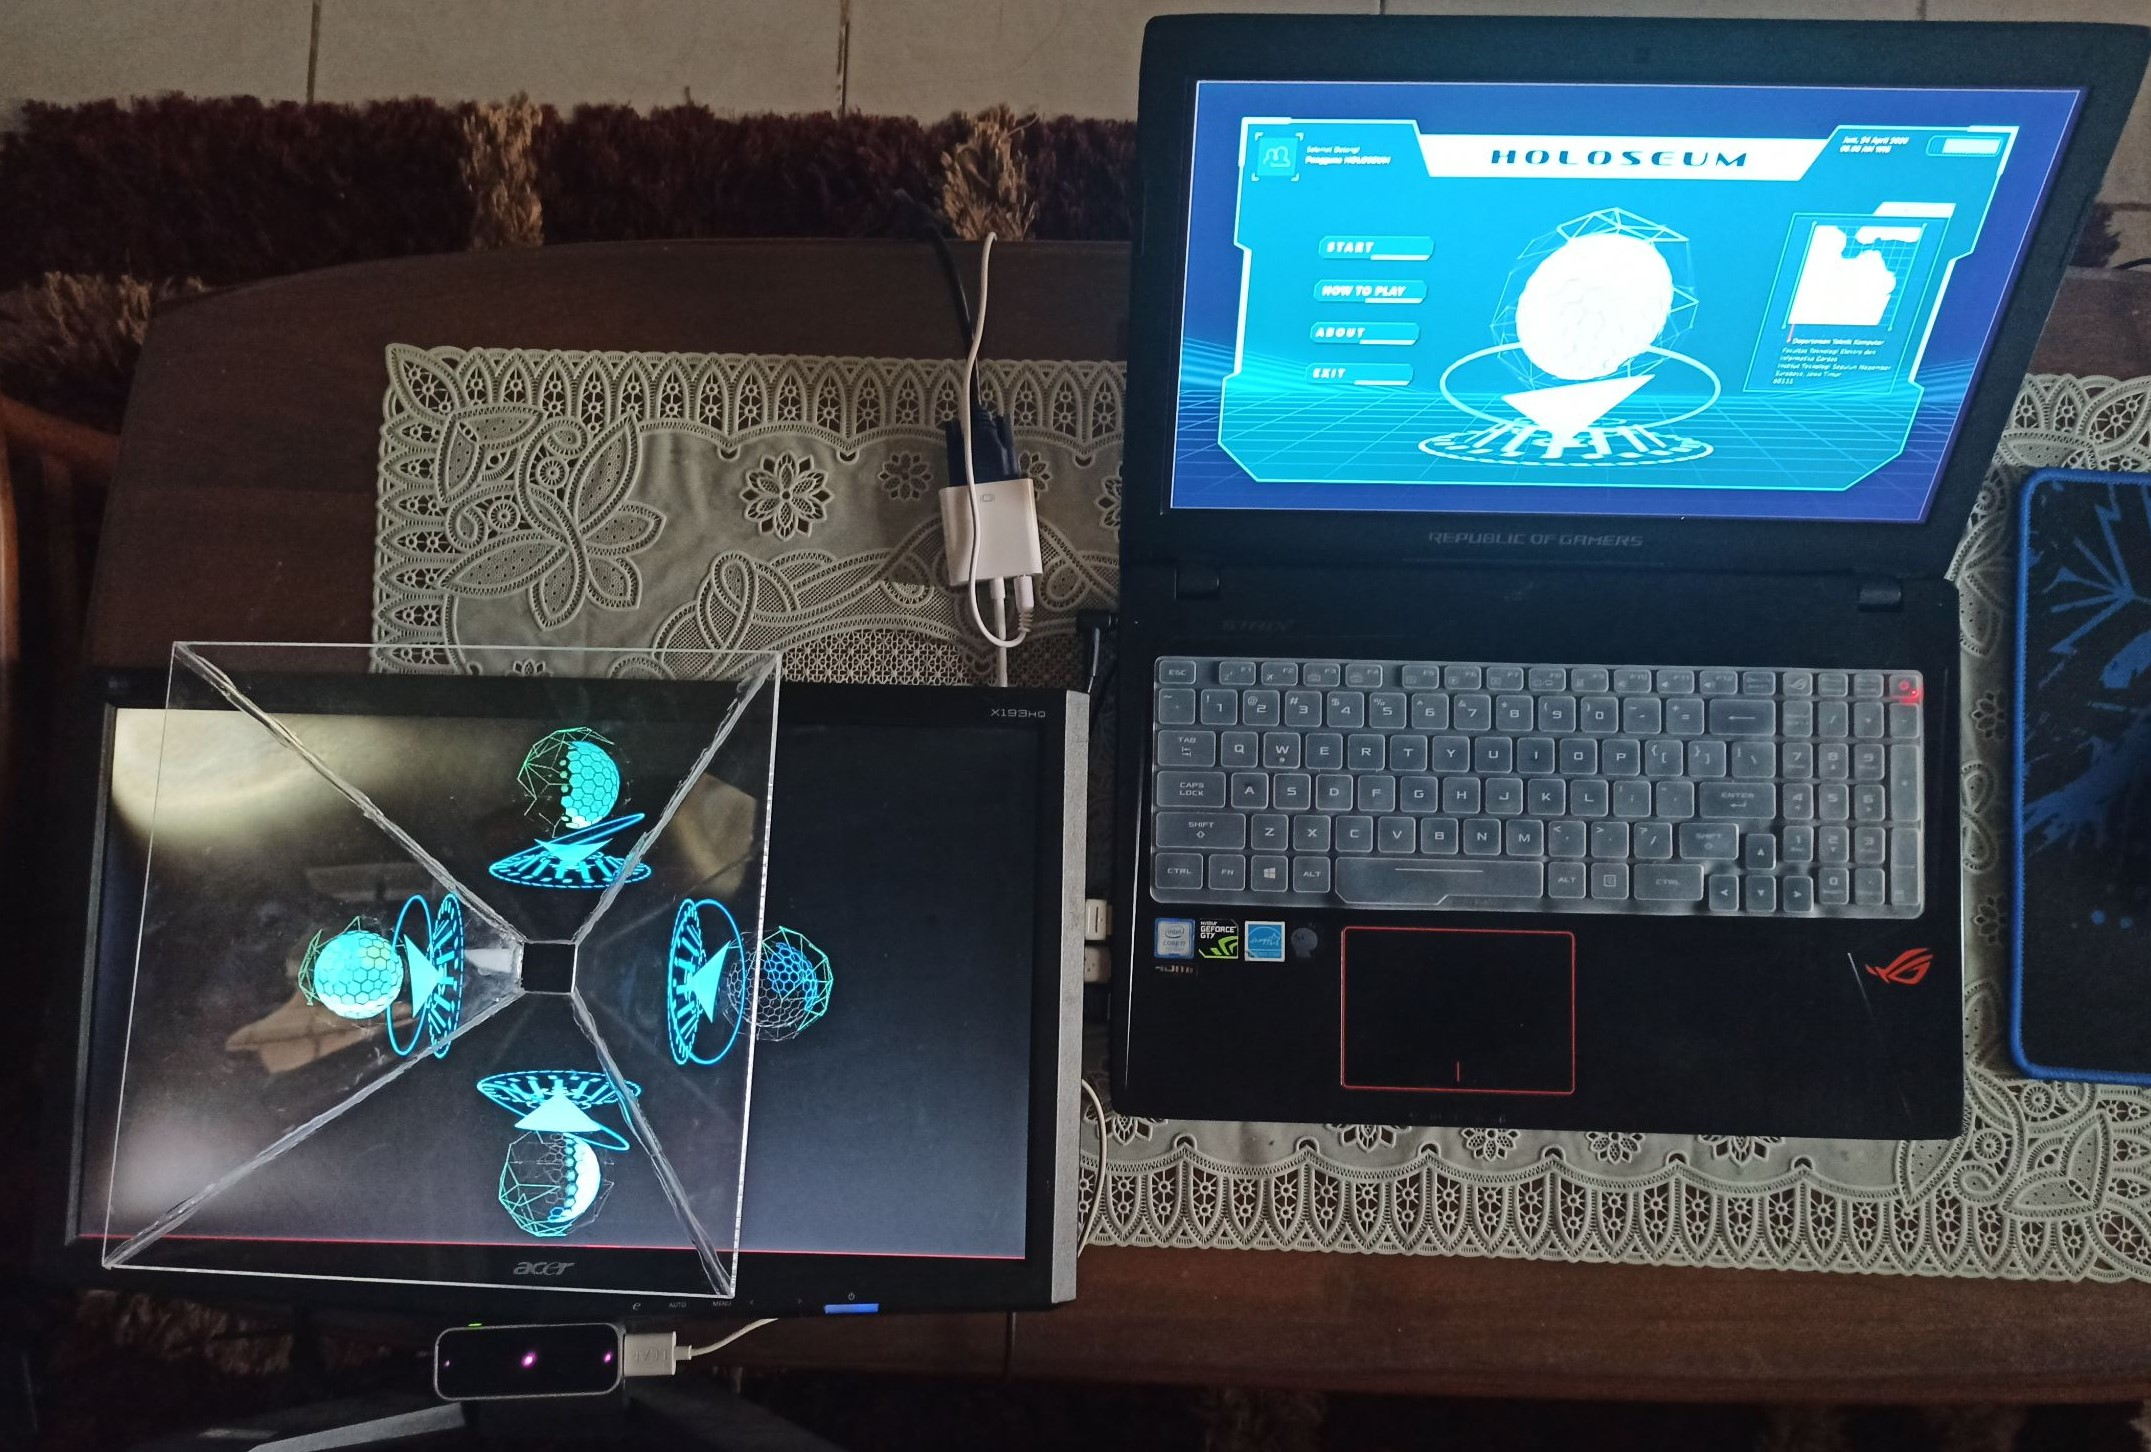
\includegraphics[width=0.33\textwidth]{img/foto_alat.jpg}}
			\caption{Device setting.}
			\label{fig:foto_alat}
		\end{figure}
		\vspace{-2ex}
	
	\subsection{Visualization System}
		The visualization system applied in this study relates to the presentation of the program on display and the server computer. The flow in building this visualization system is shown in the figure \ref{fig:desain_visualisasi}.
		
		Adjustment of 3D objects occurs through several processes. The first process is modifying object details based on their constituent elements, such as adding or subtracting constituent elements and moving their midpoints. The second process aims to arrange objects and build complementary features. The object that has been import is positioned in the middle of the camera setting and is resized via scale. Then set the default values, add the rigid body and collider components so that they can interact with the Leap Motion asset and build response features based on their gestures. The last adjustment was made to provide a holographic effect on 3D object material. 
		
		\vspace{-2ex}
		\begin{figure}[h]
			\centering{
\includegraphics[width=0.49\textwidth]{img/desain_visualisasi.png}}
			\caption{Visualization system workflow.}
			\label{fig:desain_visualisasi}
			\vspace{-4ex}
		\end{figure}

		The adjusted 3D object is then reconstructed into a video hologram to adjust the display on the monitor by adjusting the placement of the 3D object right on each side of the holographic pyramid. To display 4 object positions in 1 game view like figure \ref{fig:unity_12cam}, the setting applied in this study is a 3D object surrounded by 4 different main cameras and 7 hidden cameras to display a black background.
		\vspace{-2ex}
		\begin{figure}[h]
			\centering{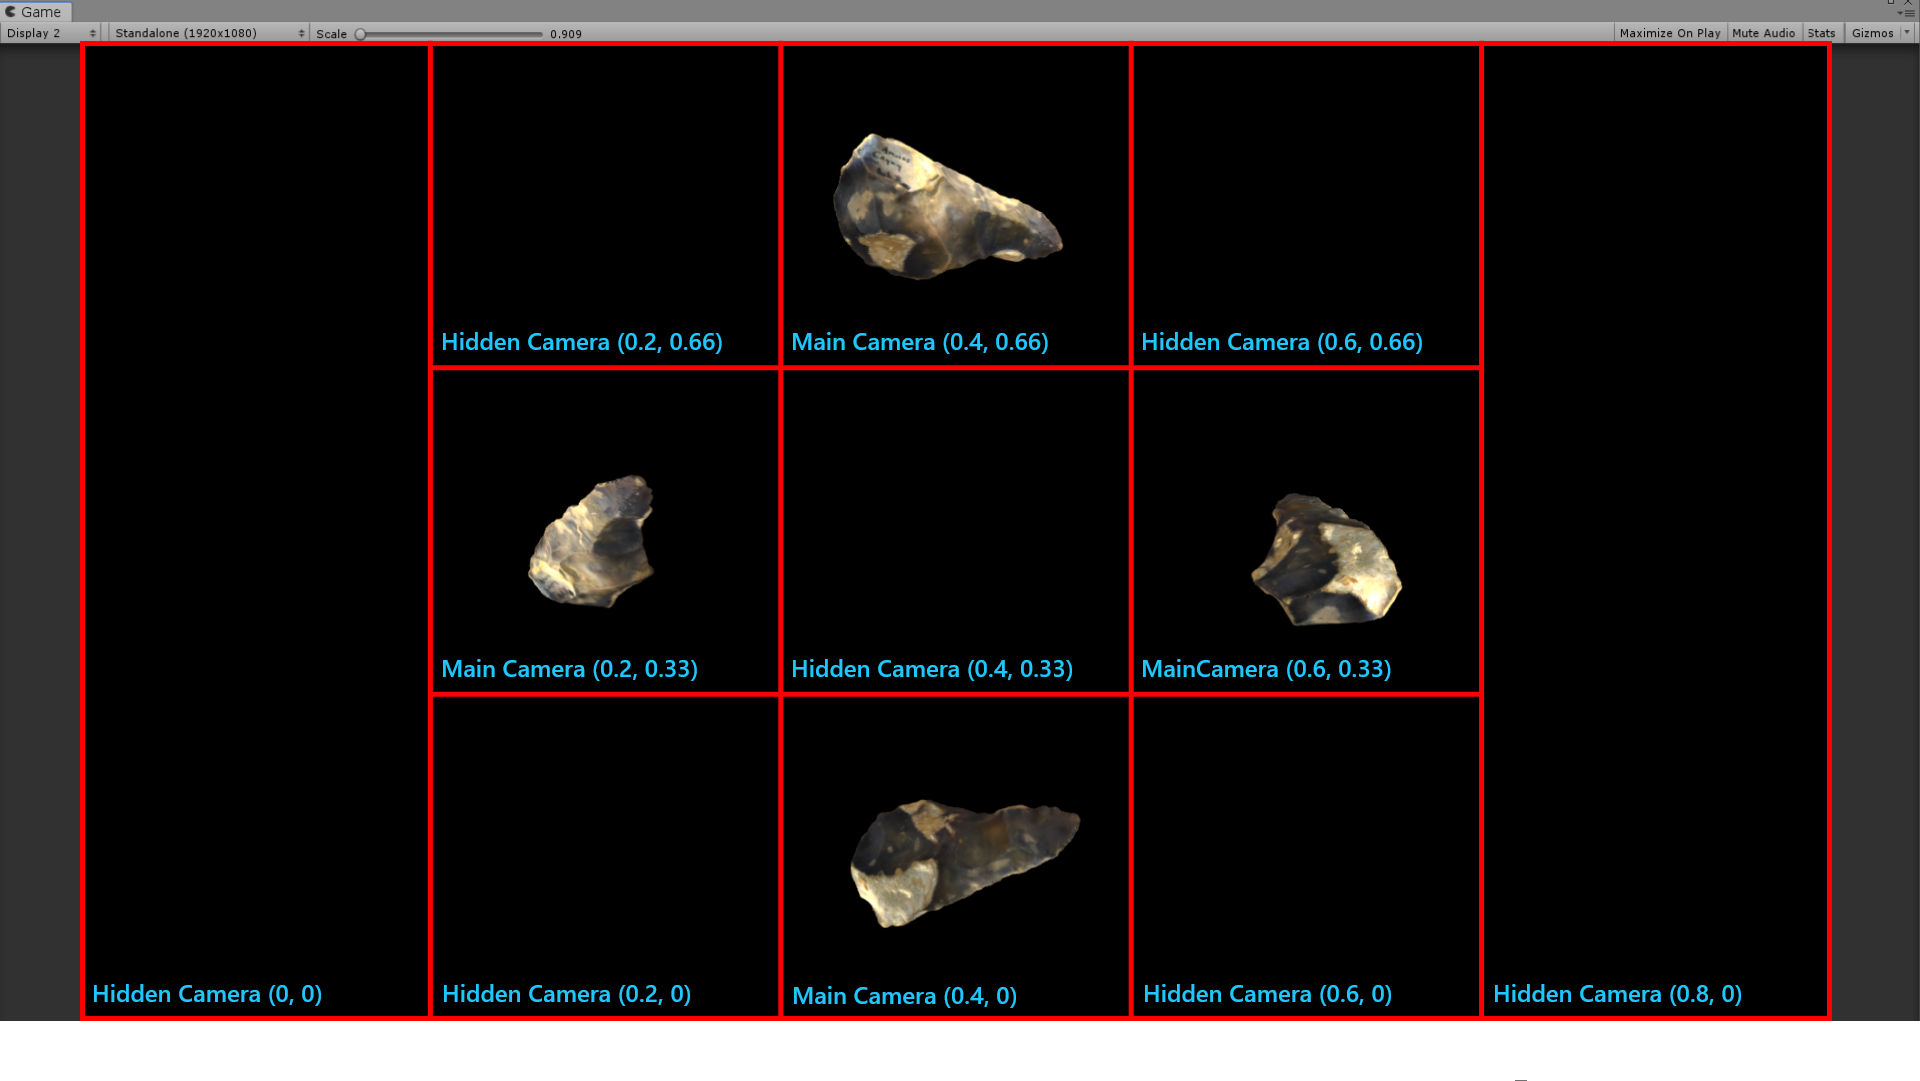
\includegraphics[width=0.4\textwidth]{img/unity_12cam.png}}
			\vspace{-1ex}
			\caption{Viewport settings for video holograms.}
			\label{fig:unity_12cam}
		\end{figure}
		\vspace{-2ex}
		
		The object displayed on the monitor display also displays its information through the monitor information. The first part of the Main Menu or Main Menu is the initial display when the application is run. Consists of the Start button to go to the Main Scene, How to Play to show how to play, About to show information about products and developers, and Exit to exit the application shown in the figure \ref{fig:mainmenu}.
		
		\vspace{-2ex}
		\begin{figure} [h]
			\begin{subfigure}{0.23\textwidth}
				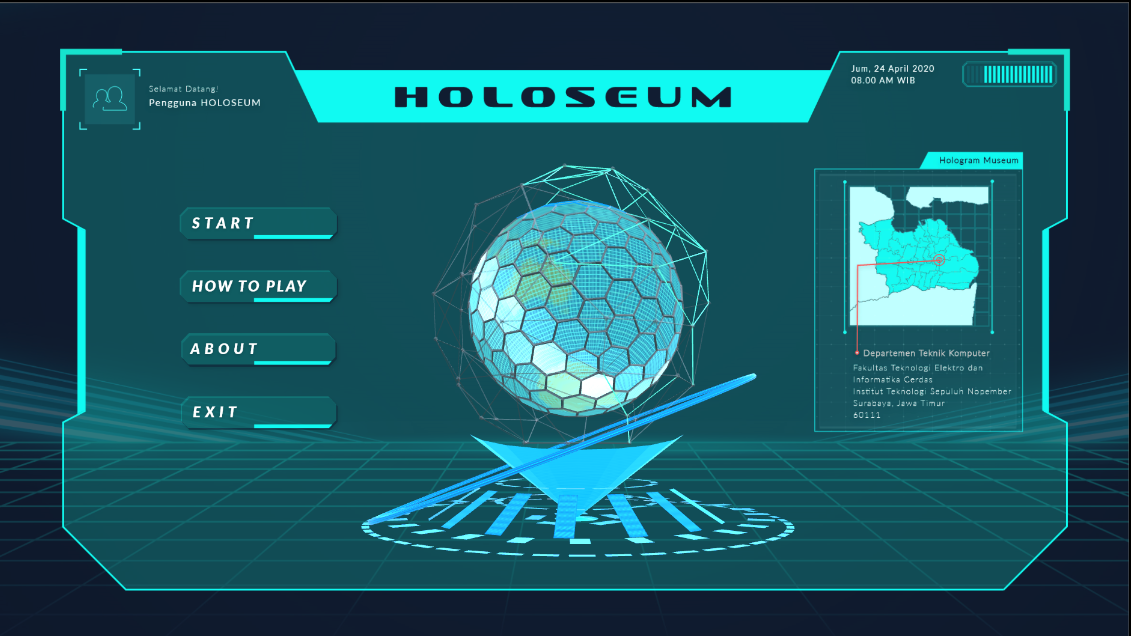
\includegraphics[width=\textwidth]{img/mainmenu.png}
				\caption{Main Menu.\label{fig:mainmenu}}
			\end{subfigure}
			\hspace{0.1em}
			\begin{subfigure}{0.23\textwidth}
				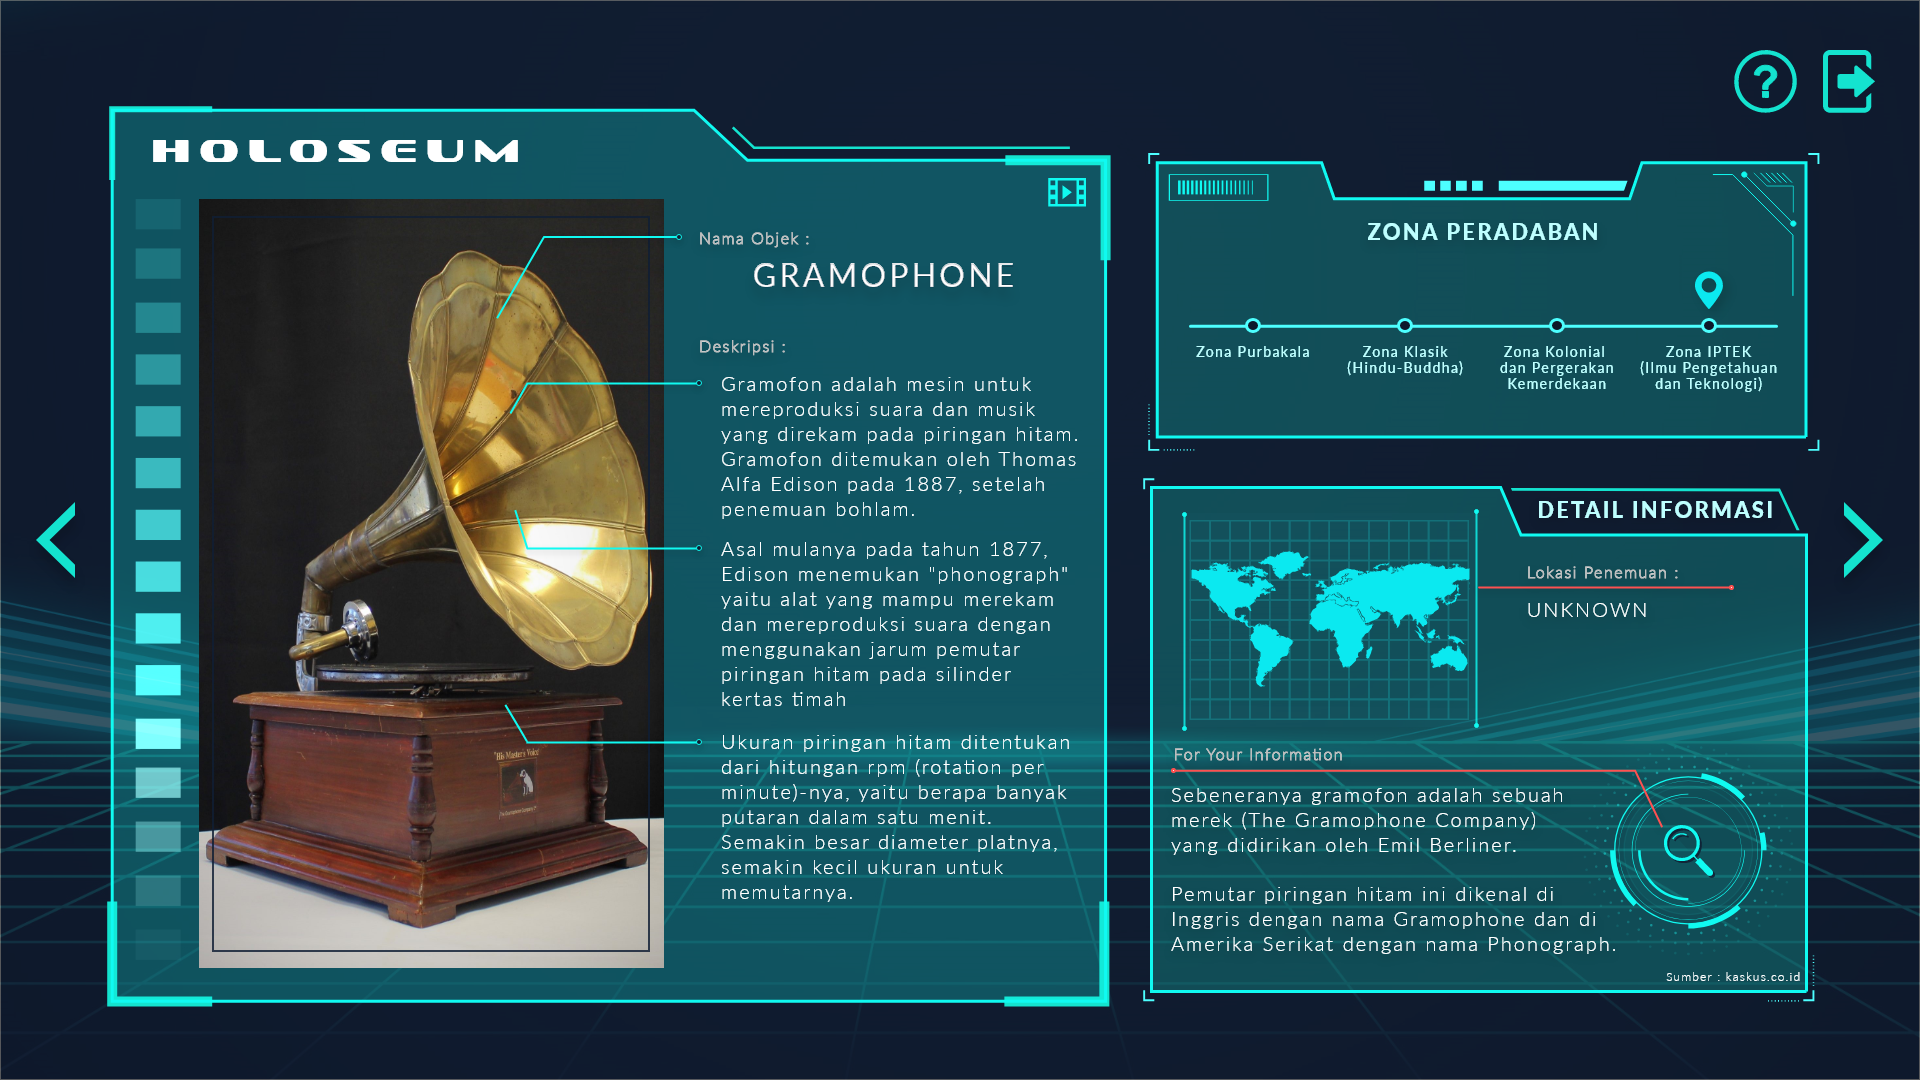
\includegraphics[width=\textwidth]{img/mainscene.png}
				\caption{Main Scene.\label{fig:mainscene}}
			\end{subfigure}
			\vspace{-1ex}
			\caption{Main interface of the application.}
		\end{figure}
		\vspace{-2ex}
		
		Whereas Main Scene is the main scene or gameplay which displays the hologram object along with the original information and photos. There are also buttons Next and Previous function to replace the displayed object, both on the monitor display and monitor information. The "animation" icon indicates whether the hologram object has an animation that can be rotated according to the corresponding gesture. 
		
	\subsection{Interaction System}
		The interaction system applied in this research is related to the process of detecting hand patterns and activating response-built features. The workflow of the interaction system that is applied is shown in the figure \ref{fig:desain_interaksi}.
		\vspace{-2ex}
		\begin{figure}[h]
			\centering{
\includegraphics[width=0.49\textwidth]{img/desain_interaksi.png}}
			\caption{Interaction system workflow.}
			\label{fig:desain_interaksi}
		\end{figure}
		\vspace{-2ex}
		
		The hand pattern can be seen if the condition of each hand object elements that builds it is active. Each detector can only detect one type of element, so if you want to detect several elements at once you need a logic gate detector like logic gate AND and OR as well as the negation. Hand gestures built in this study were shown through the figure \ref{fig:gestur_interaksi}.
	
	\subsubsection{Object Exploration Algorithm}
		Object exploration that can be done by the user is by grasping the object to see holographic objects from all sides using the \ref{fig:gs1a} and \ref{fig:gs1b} gestures. The explored hologram object will respond to rotating gestures on its axis and move to a predetermined area based on changes in position and rotation of the hand obtained from the movement (difference) between frames. The equation \ref{eqn:position_target} is used to calculate the position value while the equation \ref{eqn:rotation_target} is to get the rotation value.
					\vspace{-2ex}			
		\begin{equation}
		\begin{alignedat}{2}
		& \overrightarrow{V_{C}} &&= \overrightarrow{V_{B}} - \overrightarrow{V_{A}}\\
		%& 		&&= (V_{B}.x - V_{A}.x, V_{B}.y - V_{A}.y, V_{B}.z - V_{A}.z)\\
		& 		&&= (\overrightarrow{V_{B}}.x - \overrightarrow{V_{A}}.x, \overrightarrow{V_{B}}.y - \overrightarrow{V_{A}}.y, \overrightarrow{V_{B}}.z - \overrightarrow{V_{A}}.z)\\
		%& 		&&= ({V_{B}}_{x} \uvec{i} - {V_{A}}_{x} \uvec{i}, {V_{B}}_{y} \uvec{j} - {V_{A}}_{y} \uvec{j}, {V_{B}}_{z} \uvec{k} - {V_{A}}_{z} \uvec{k})
		%& 		&&= (x_{\overrightarrow{V_{B}}} - x_{\overrightarrow{V_{A}}}, y_{\overrightarrow{V_{B}}} - y_{\overrightarrow{V_{A}}}, z_{\overrightarrow{V_{B}}} - z_{\overrightarrow{V_{A}}})\\	
		\end{alignedat}
		\label{eqn:position_target}
		\end{equation}
		
		\begin{equation}
		\begin{alignedat}{3}
		\overrightarrow{Q_{A}} \cdot & \overrightarrow{Q_{C}} &&= \overrightarrow{Q_{B}}\\ 
		\overrightarrow{Q_{A}} \cdot \overrightarrow{\inv{Q_{A}}} \cdot& \overrightarrow{Q_{C}} &&= \overrightarrow{\inv{Q_{A}}} \cdot \overrightarrow{Q_{B}}\\
		\overrightarrow{I} \cdot & \overrightarrow{Q_{C}} &&= \overrightarrow{\inv{Q_{A}}} \cdot \overrightarrow{Q_{B}}\\
		&\overrightarrow{Q_{C}} &&= \overrightarrow{\inv{Q_{A}}} \cdot \overrightarrow{Q_{B}}\\
		\end{alignedat}
		\label{eqn:rotation_target}
		\end{equation}
	
	\subsubsection{Zoom Object Algorithm}
		Zoom Object is a feature that can zoom in and out of the hologram object until it reaches the maximum value that has been determined via \ref{fig:gs2} gesture. This feature helps users to see object details in different sizes based on the distance between the two hands represented by the index finger. The distance between the two hands is used to calculate the magnification scale ratio according to the \ref{eqn:zoom_scale} equation.
		\begin{equation}
			ScaleValue = \frac{distanceValue}{maxDistance} \cdot maxScale
			\label{eqn:zoom_scale}
		\end{equation}

	\subsubsection{Object Animation Activation Algorithm}
		This feature allows users to activate and view animated movements of the corresponding object using one of the gestures \ref{fig:gs3a}, \ref{fig:gs3b}, or \ref{fig:gs3c}. In this study, the objects which can be played are the primeval ax and gramophone that being marked by "animated" icon.

		\vspace{-2ex}
		\begin{figure} [h]
		\begin{center}
		\begin{subfigure}[t]{0.11\textwidth}
			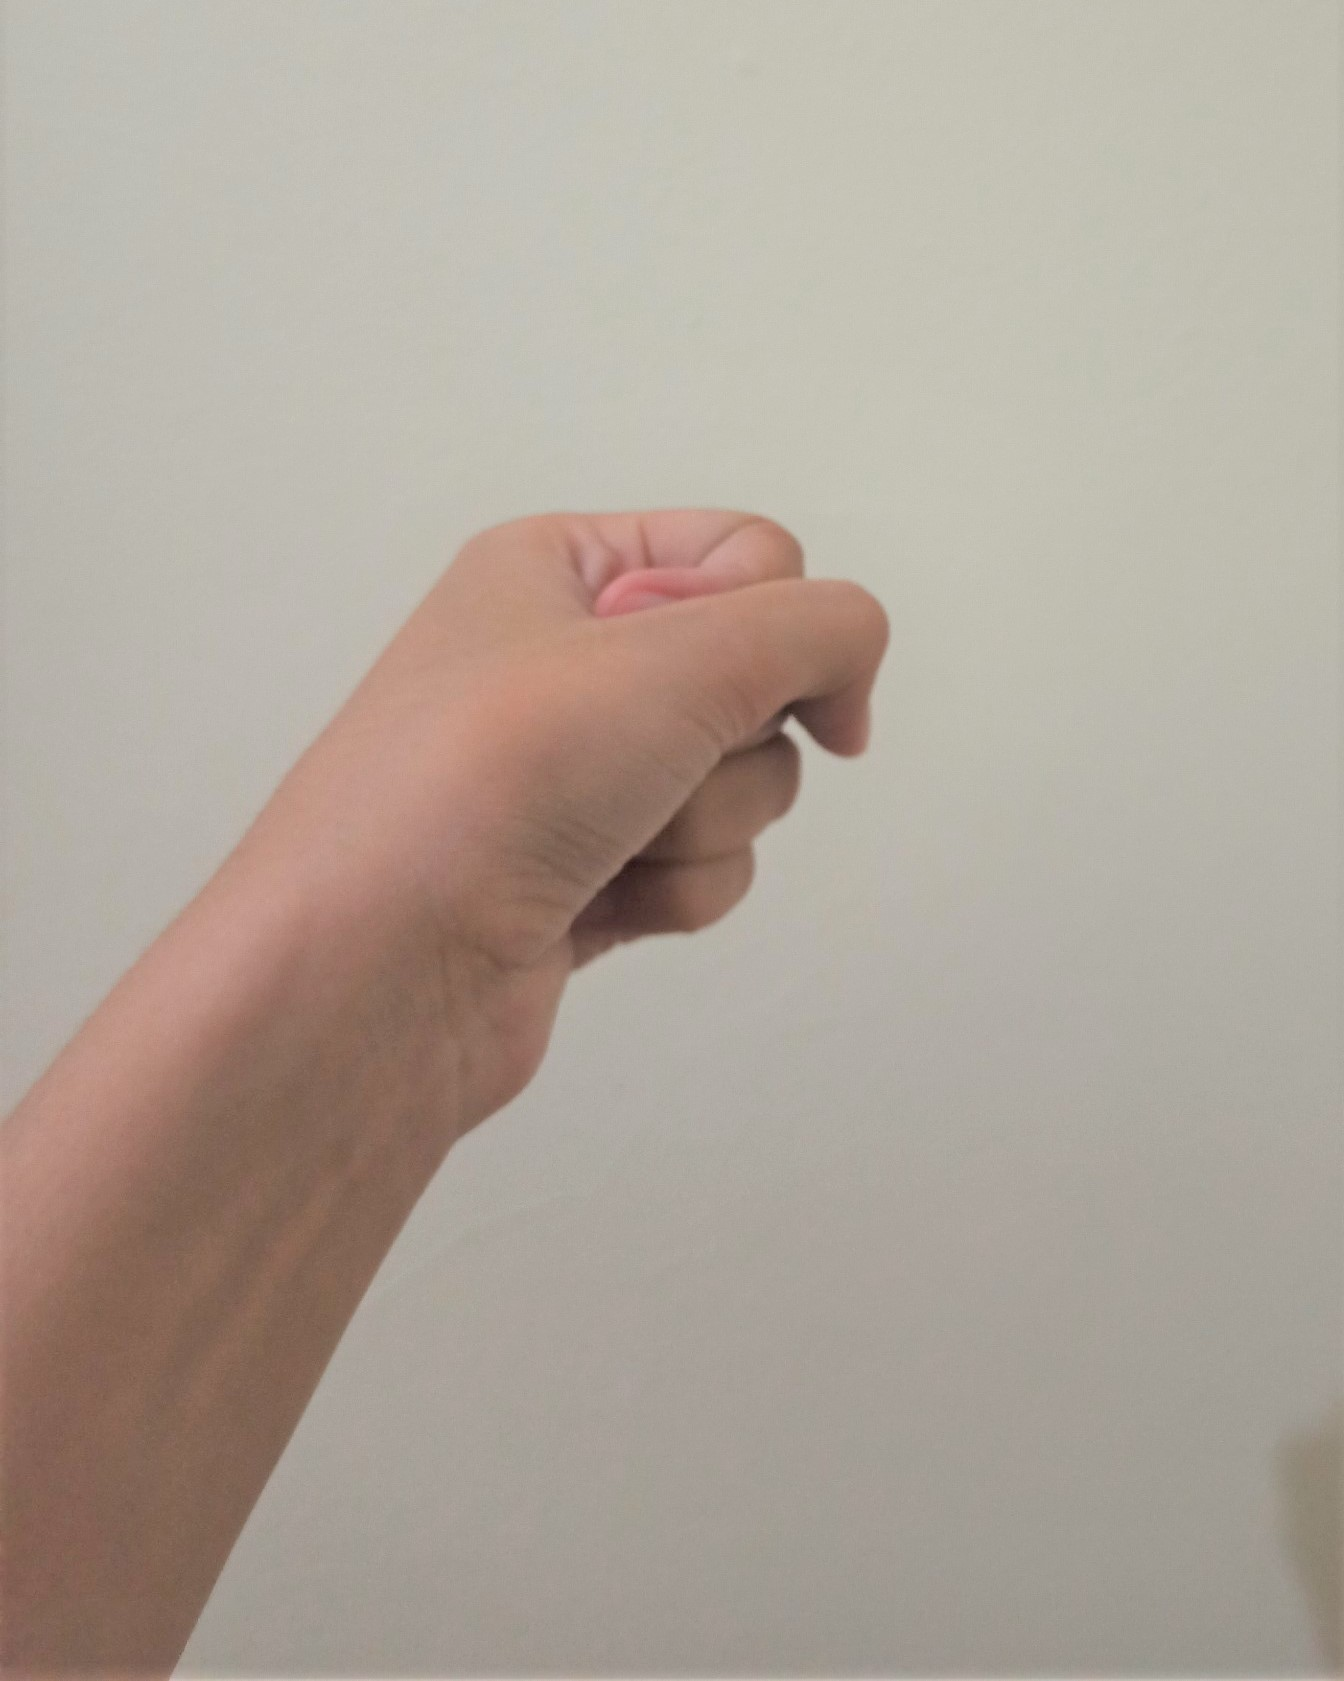
\includegraphics[width=\textwidth]{img/pola1a.jpg}
			\caption{\label{fig:gs1a}}
		\end{subfigure}
		\hspace{0.1em}
		\begin{subfigure}[t]{0.11\textwidth}
			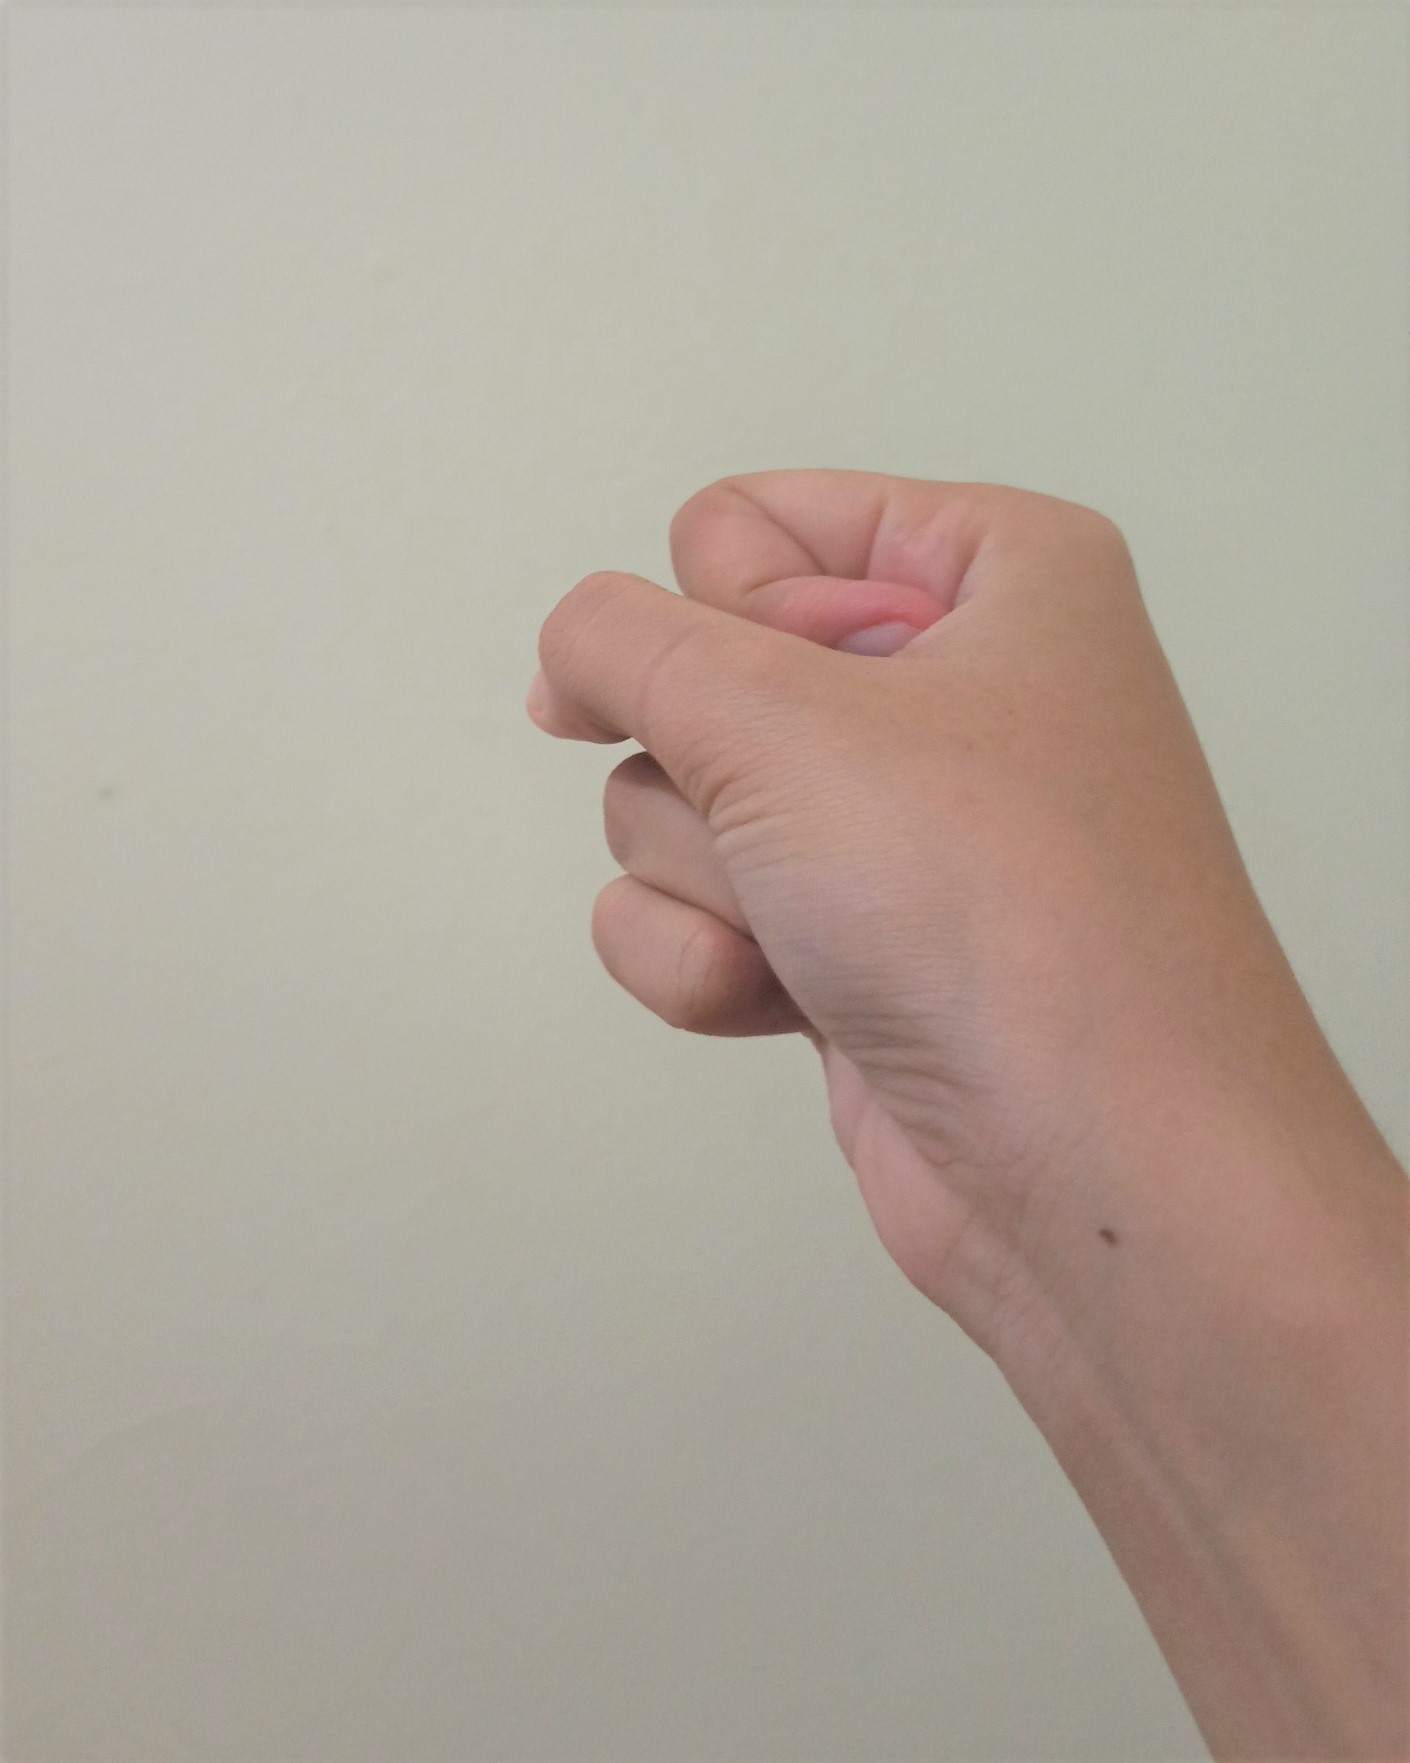
\includegraphics[width=\textwidth]{img/pola1b.jpg}
			\caption{\label{fig:gs1b}}
		\end{subfigure}
		\hspace{0.1em}
		\begin{subfigure}[t]{0.11\textwidth}
			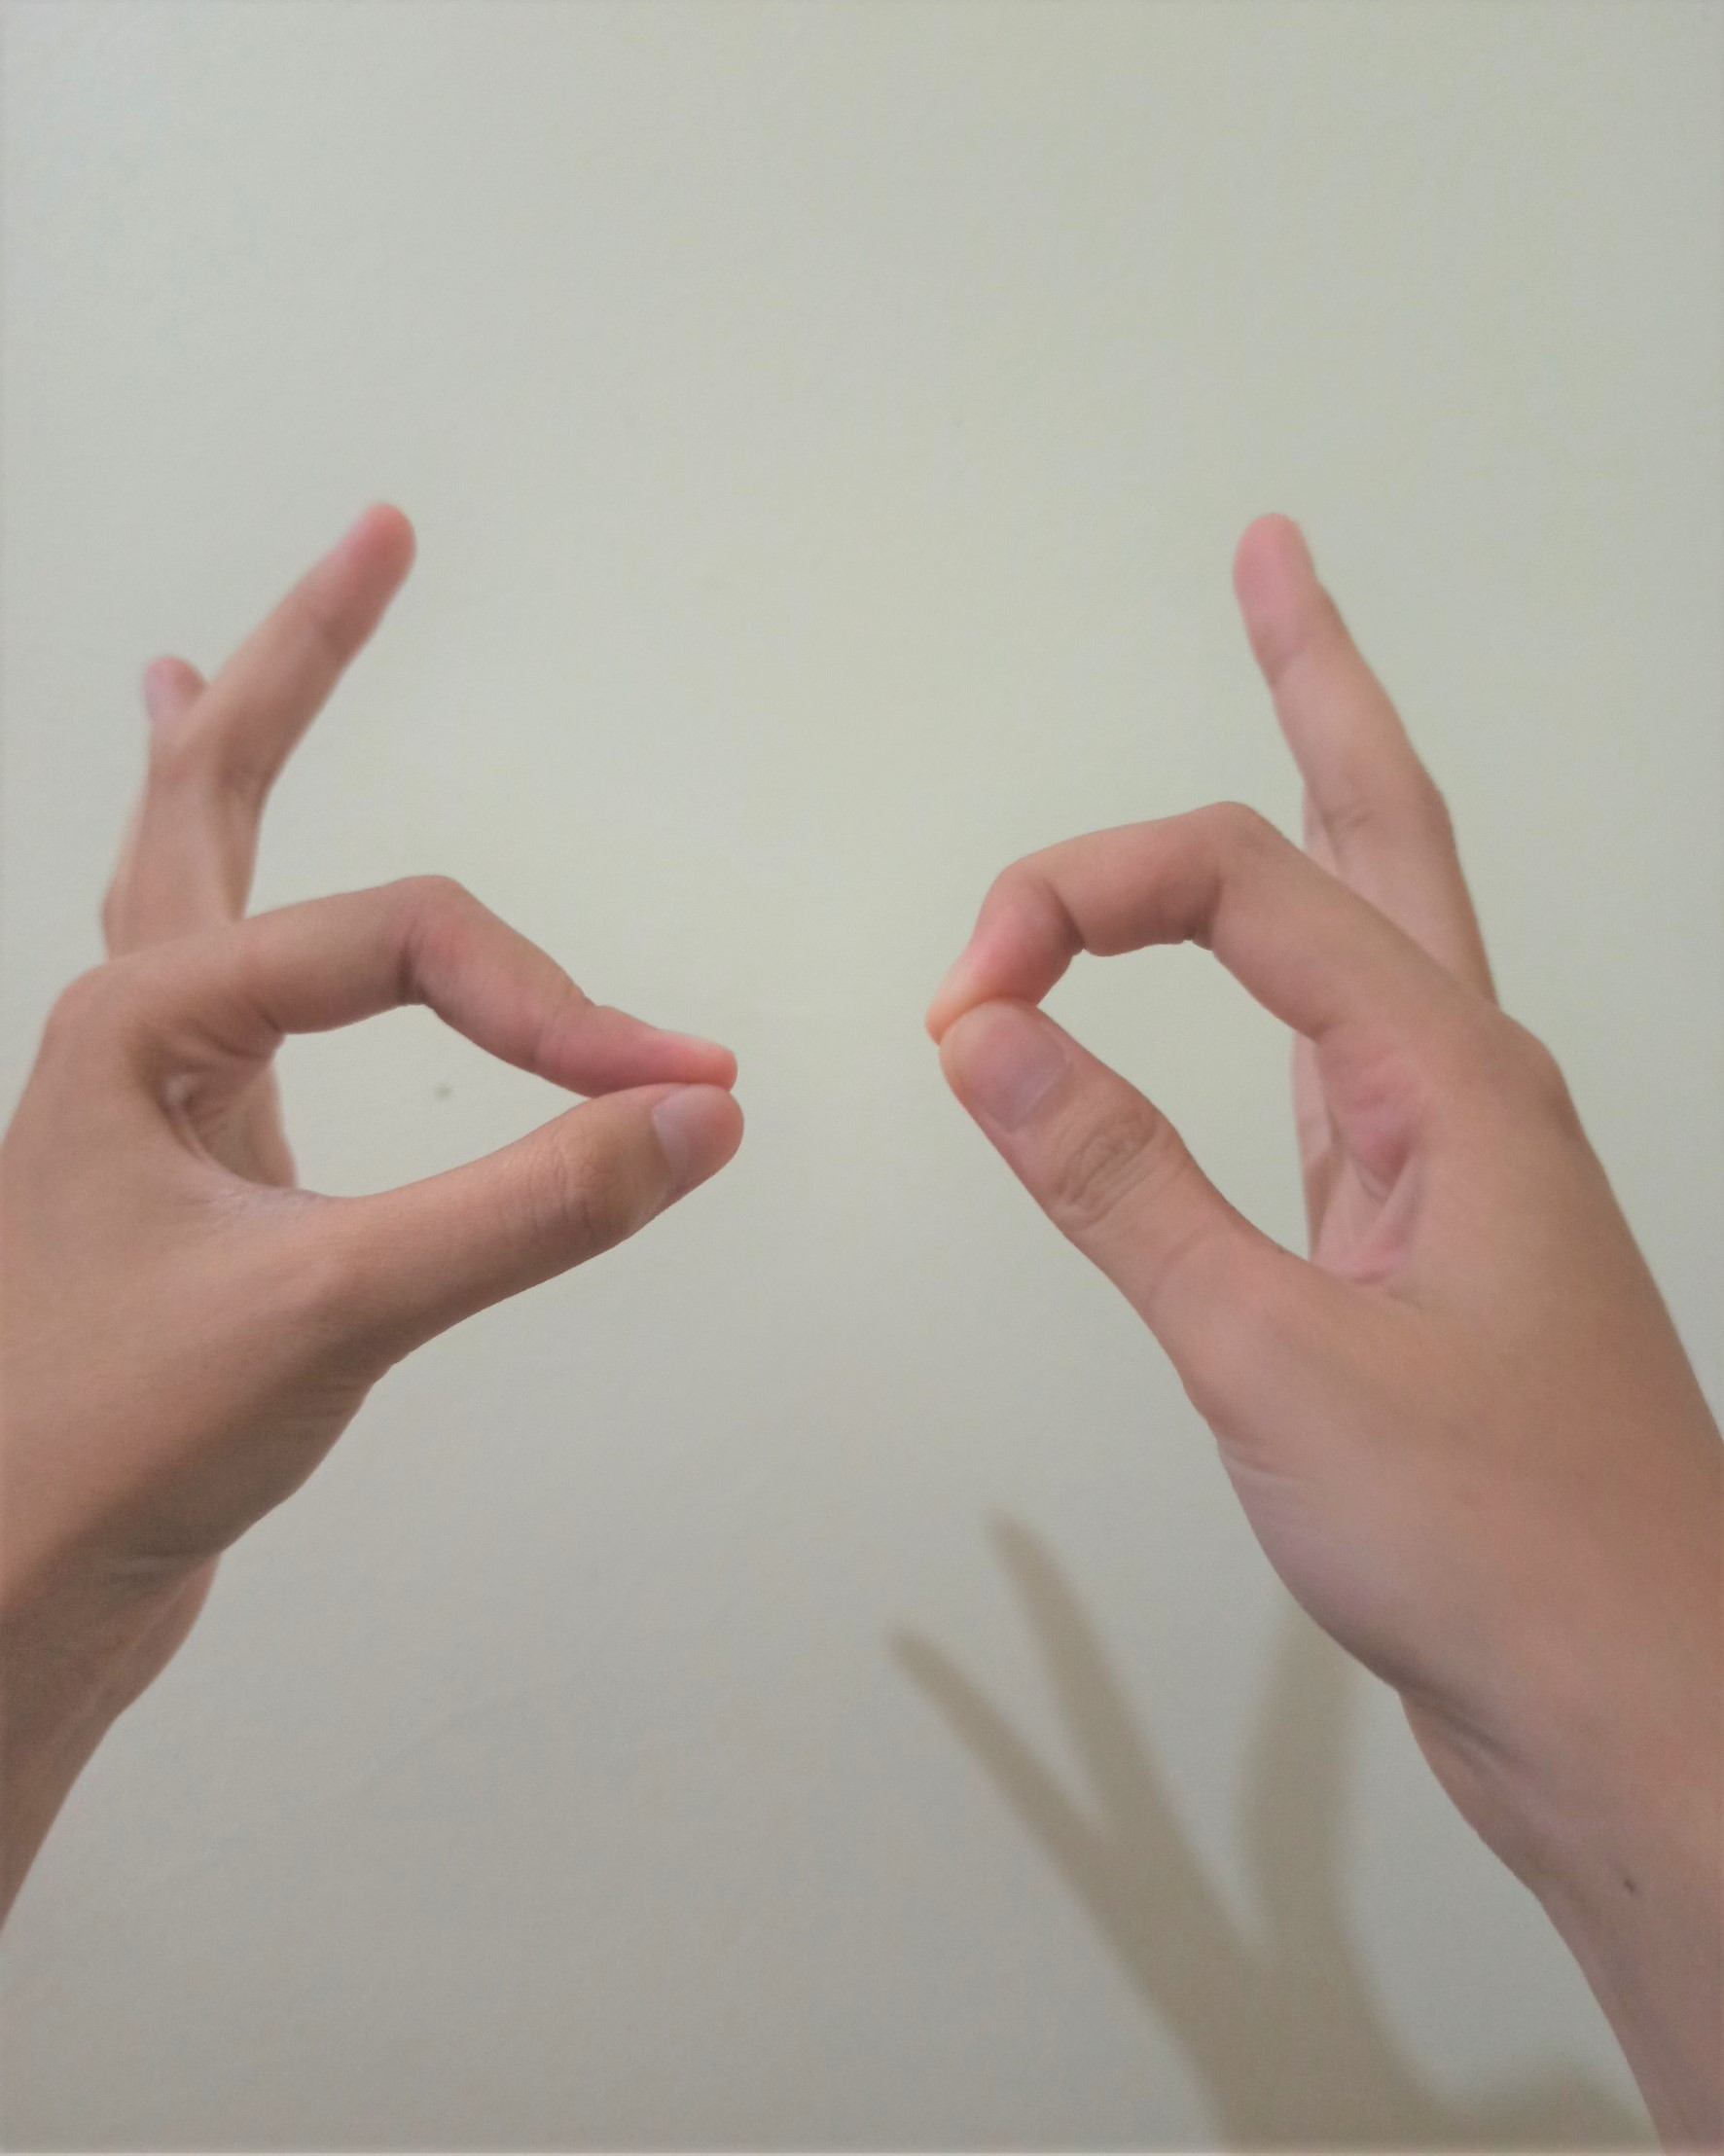
\includegraphics[width=\textwidth]{img/pola2.jpg}
			\caption{\label{fig:gs2}}
		\end{subfigure}
		\hspace{0.1em}
		\begin{subfigure}[t]{0.11\textwidth}
			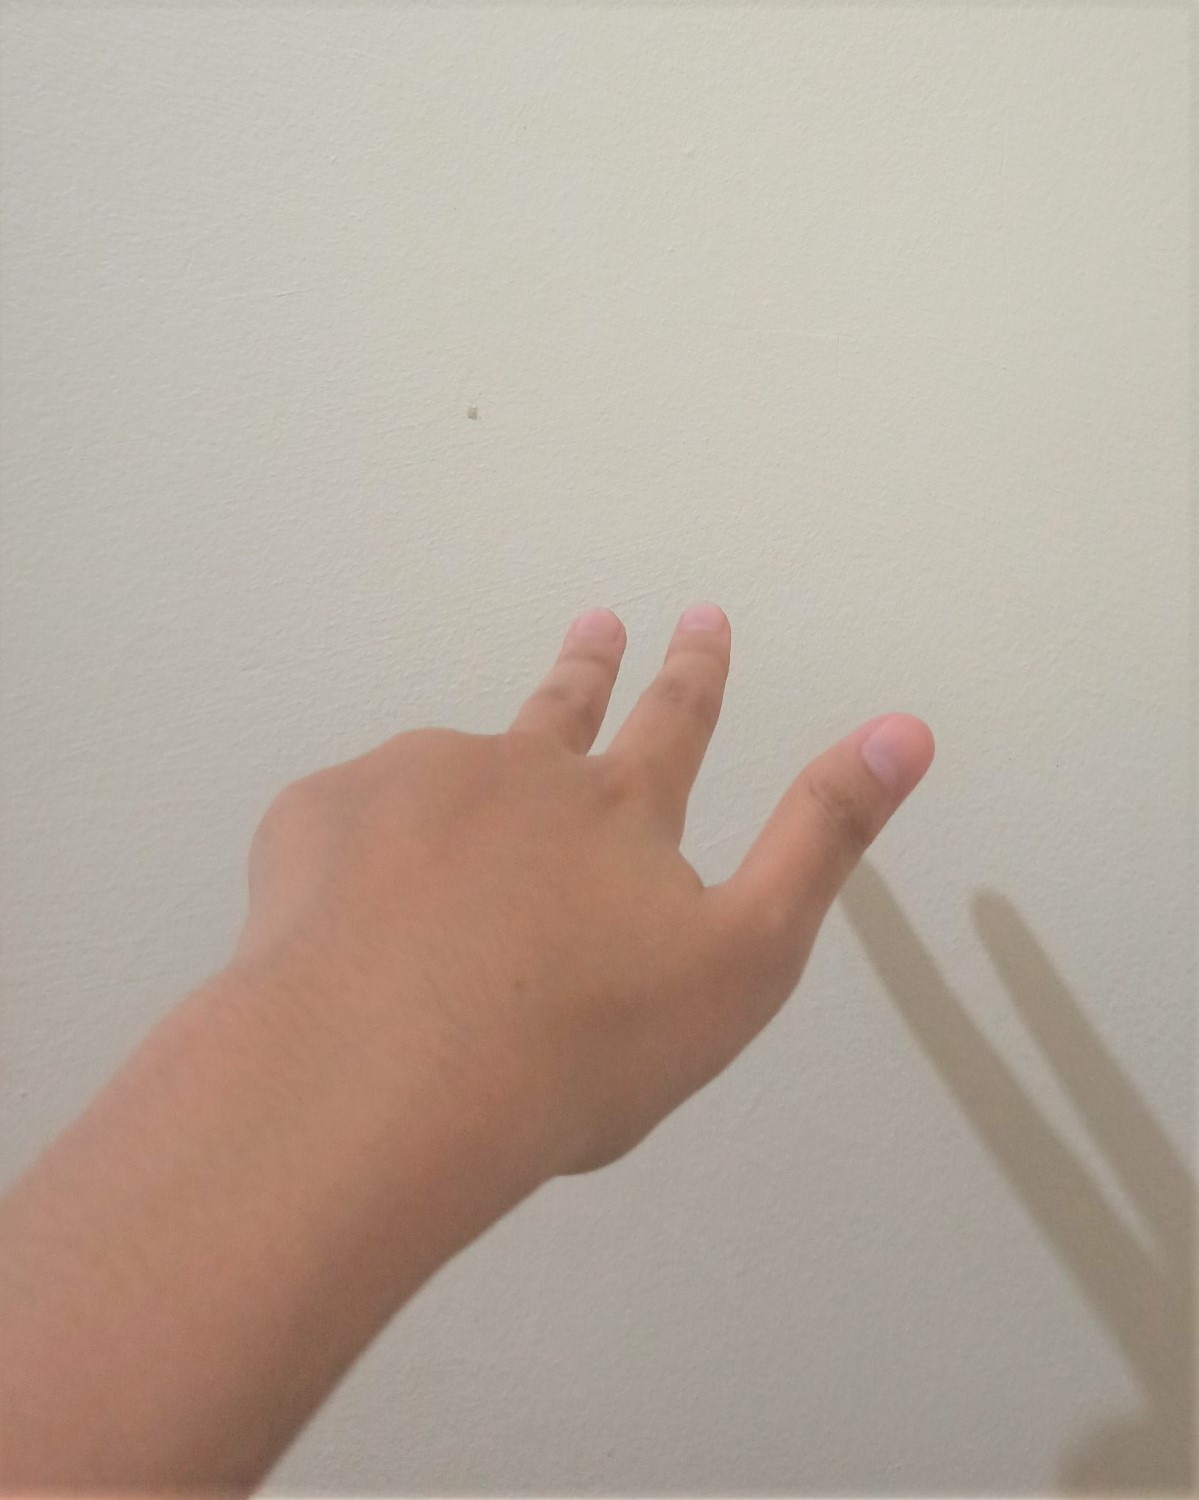
\includegraphics[width=\textwidth]{img/pola3a.jpg}
			\caption{\label{fig:gs3a}}
		\end{subfigure}
		\hspace{0.1em}
		\begin{subfigure}[t]{0.11\textwidth}
			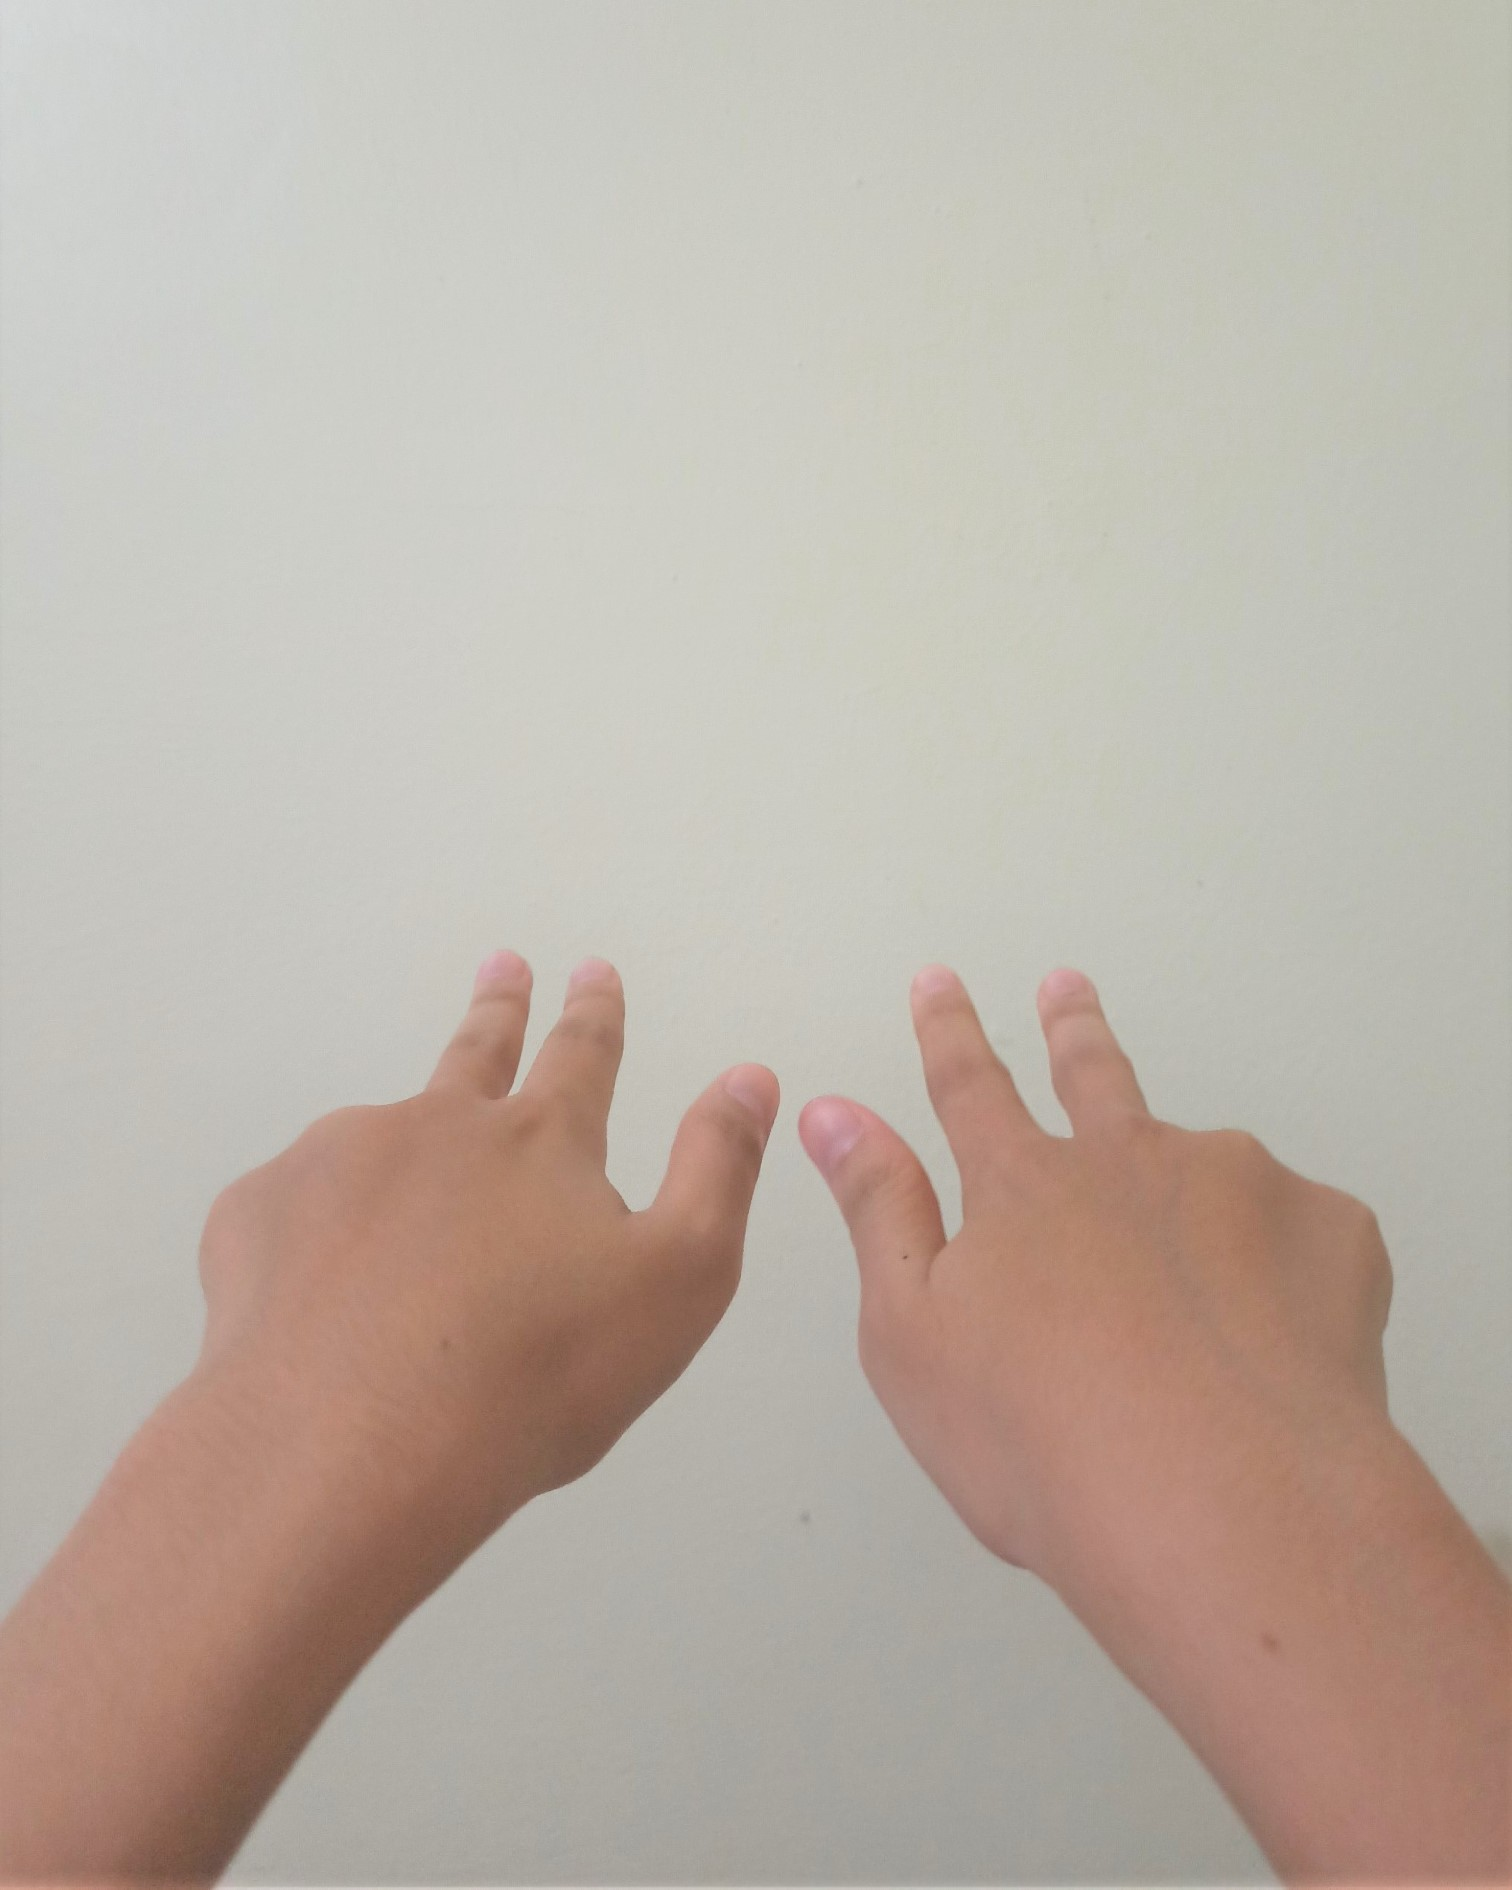
\includegraphics[width=\textwidth]{img/pola3b.jpg}
			\caption{\label{fig:gs3b}}
		\end{subfigure}
		\hspace{0.1em}
		\begin{subfigure}[t]{0.11\textwidth}
			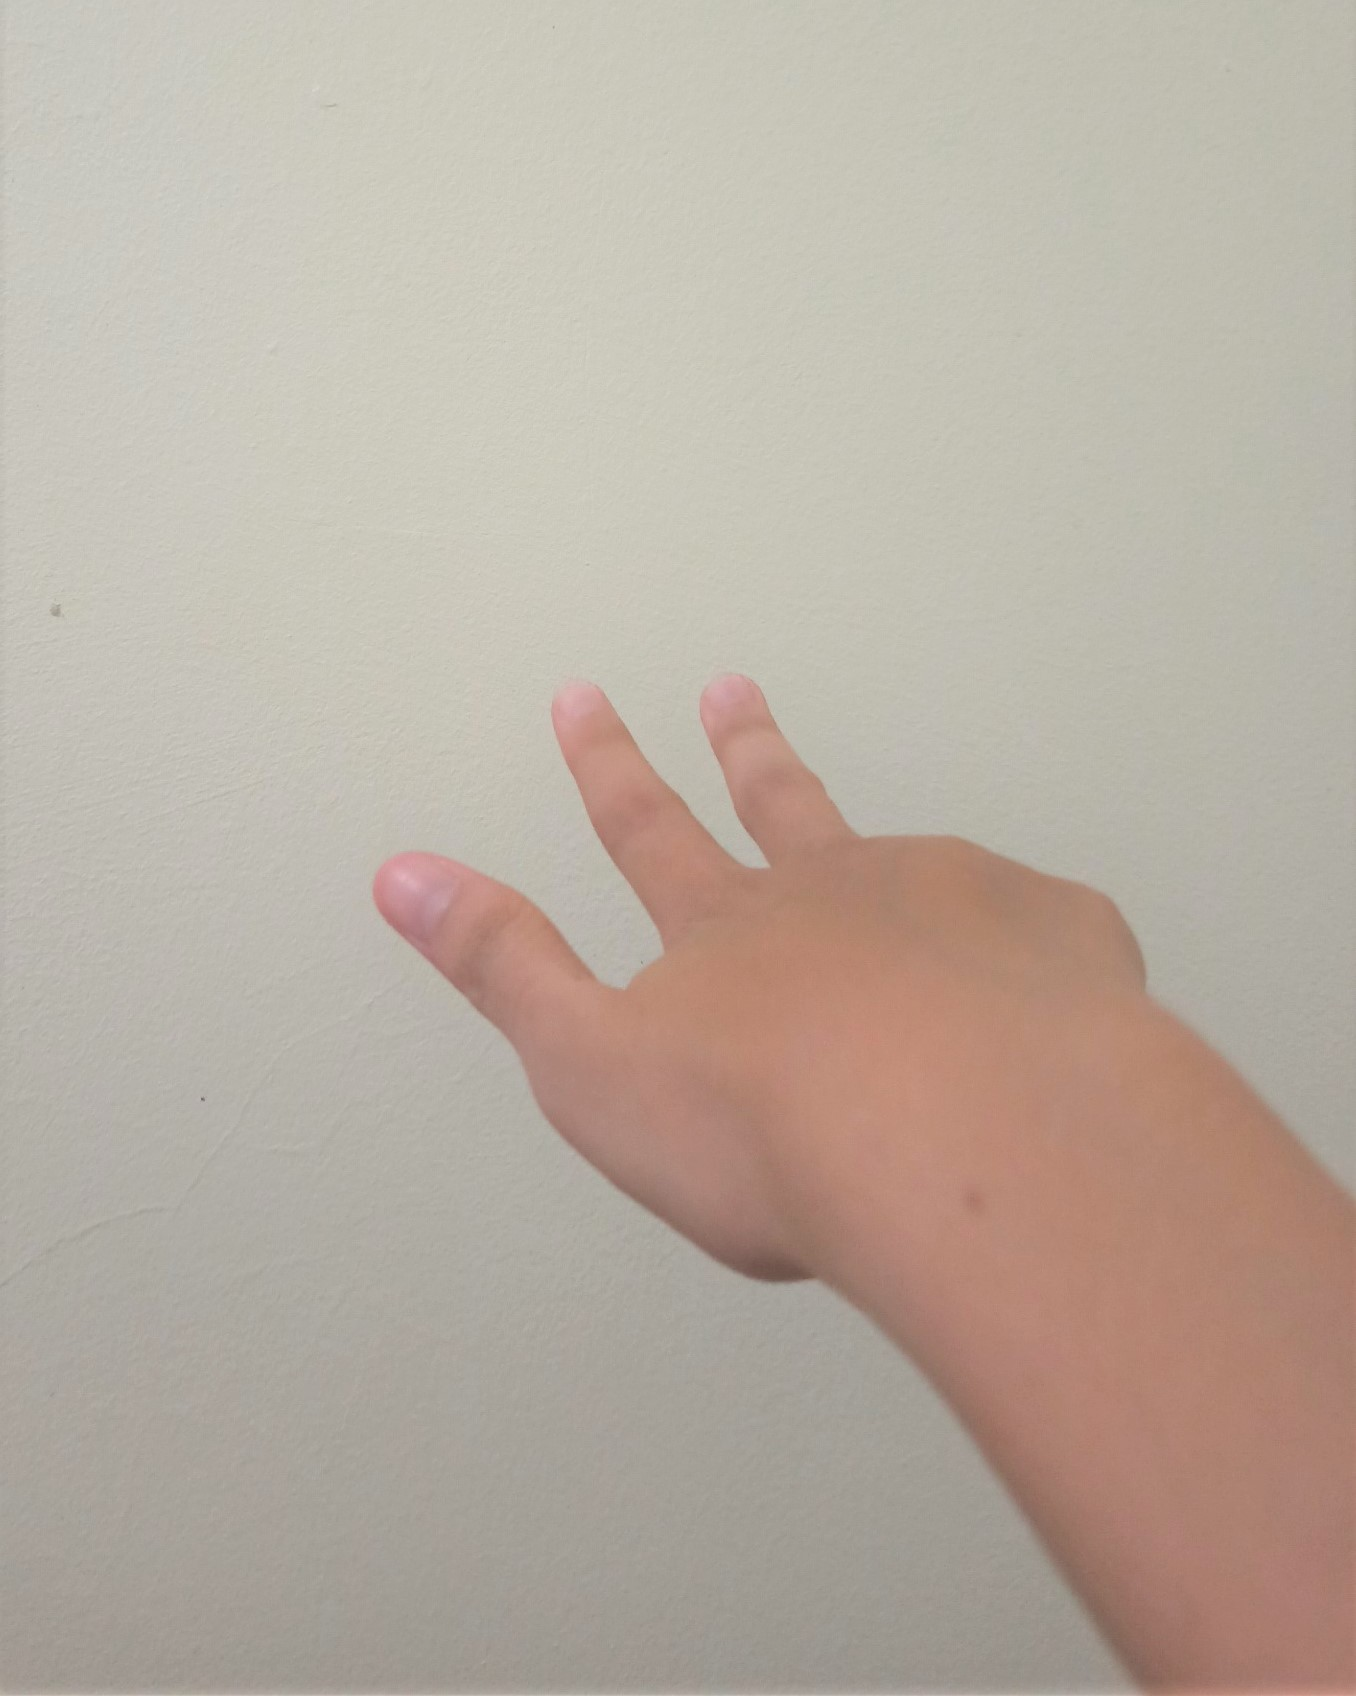
\includegraphics[width=\textwidth]{img/pola3c.jpg}
			\caption{\label{fig:gs3c}}
		\end{subfigure}
		\hspace{0.1em}
		\begin{subfigure}[t]{0.11\textwidth}
			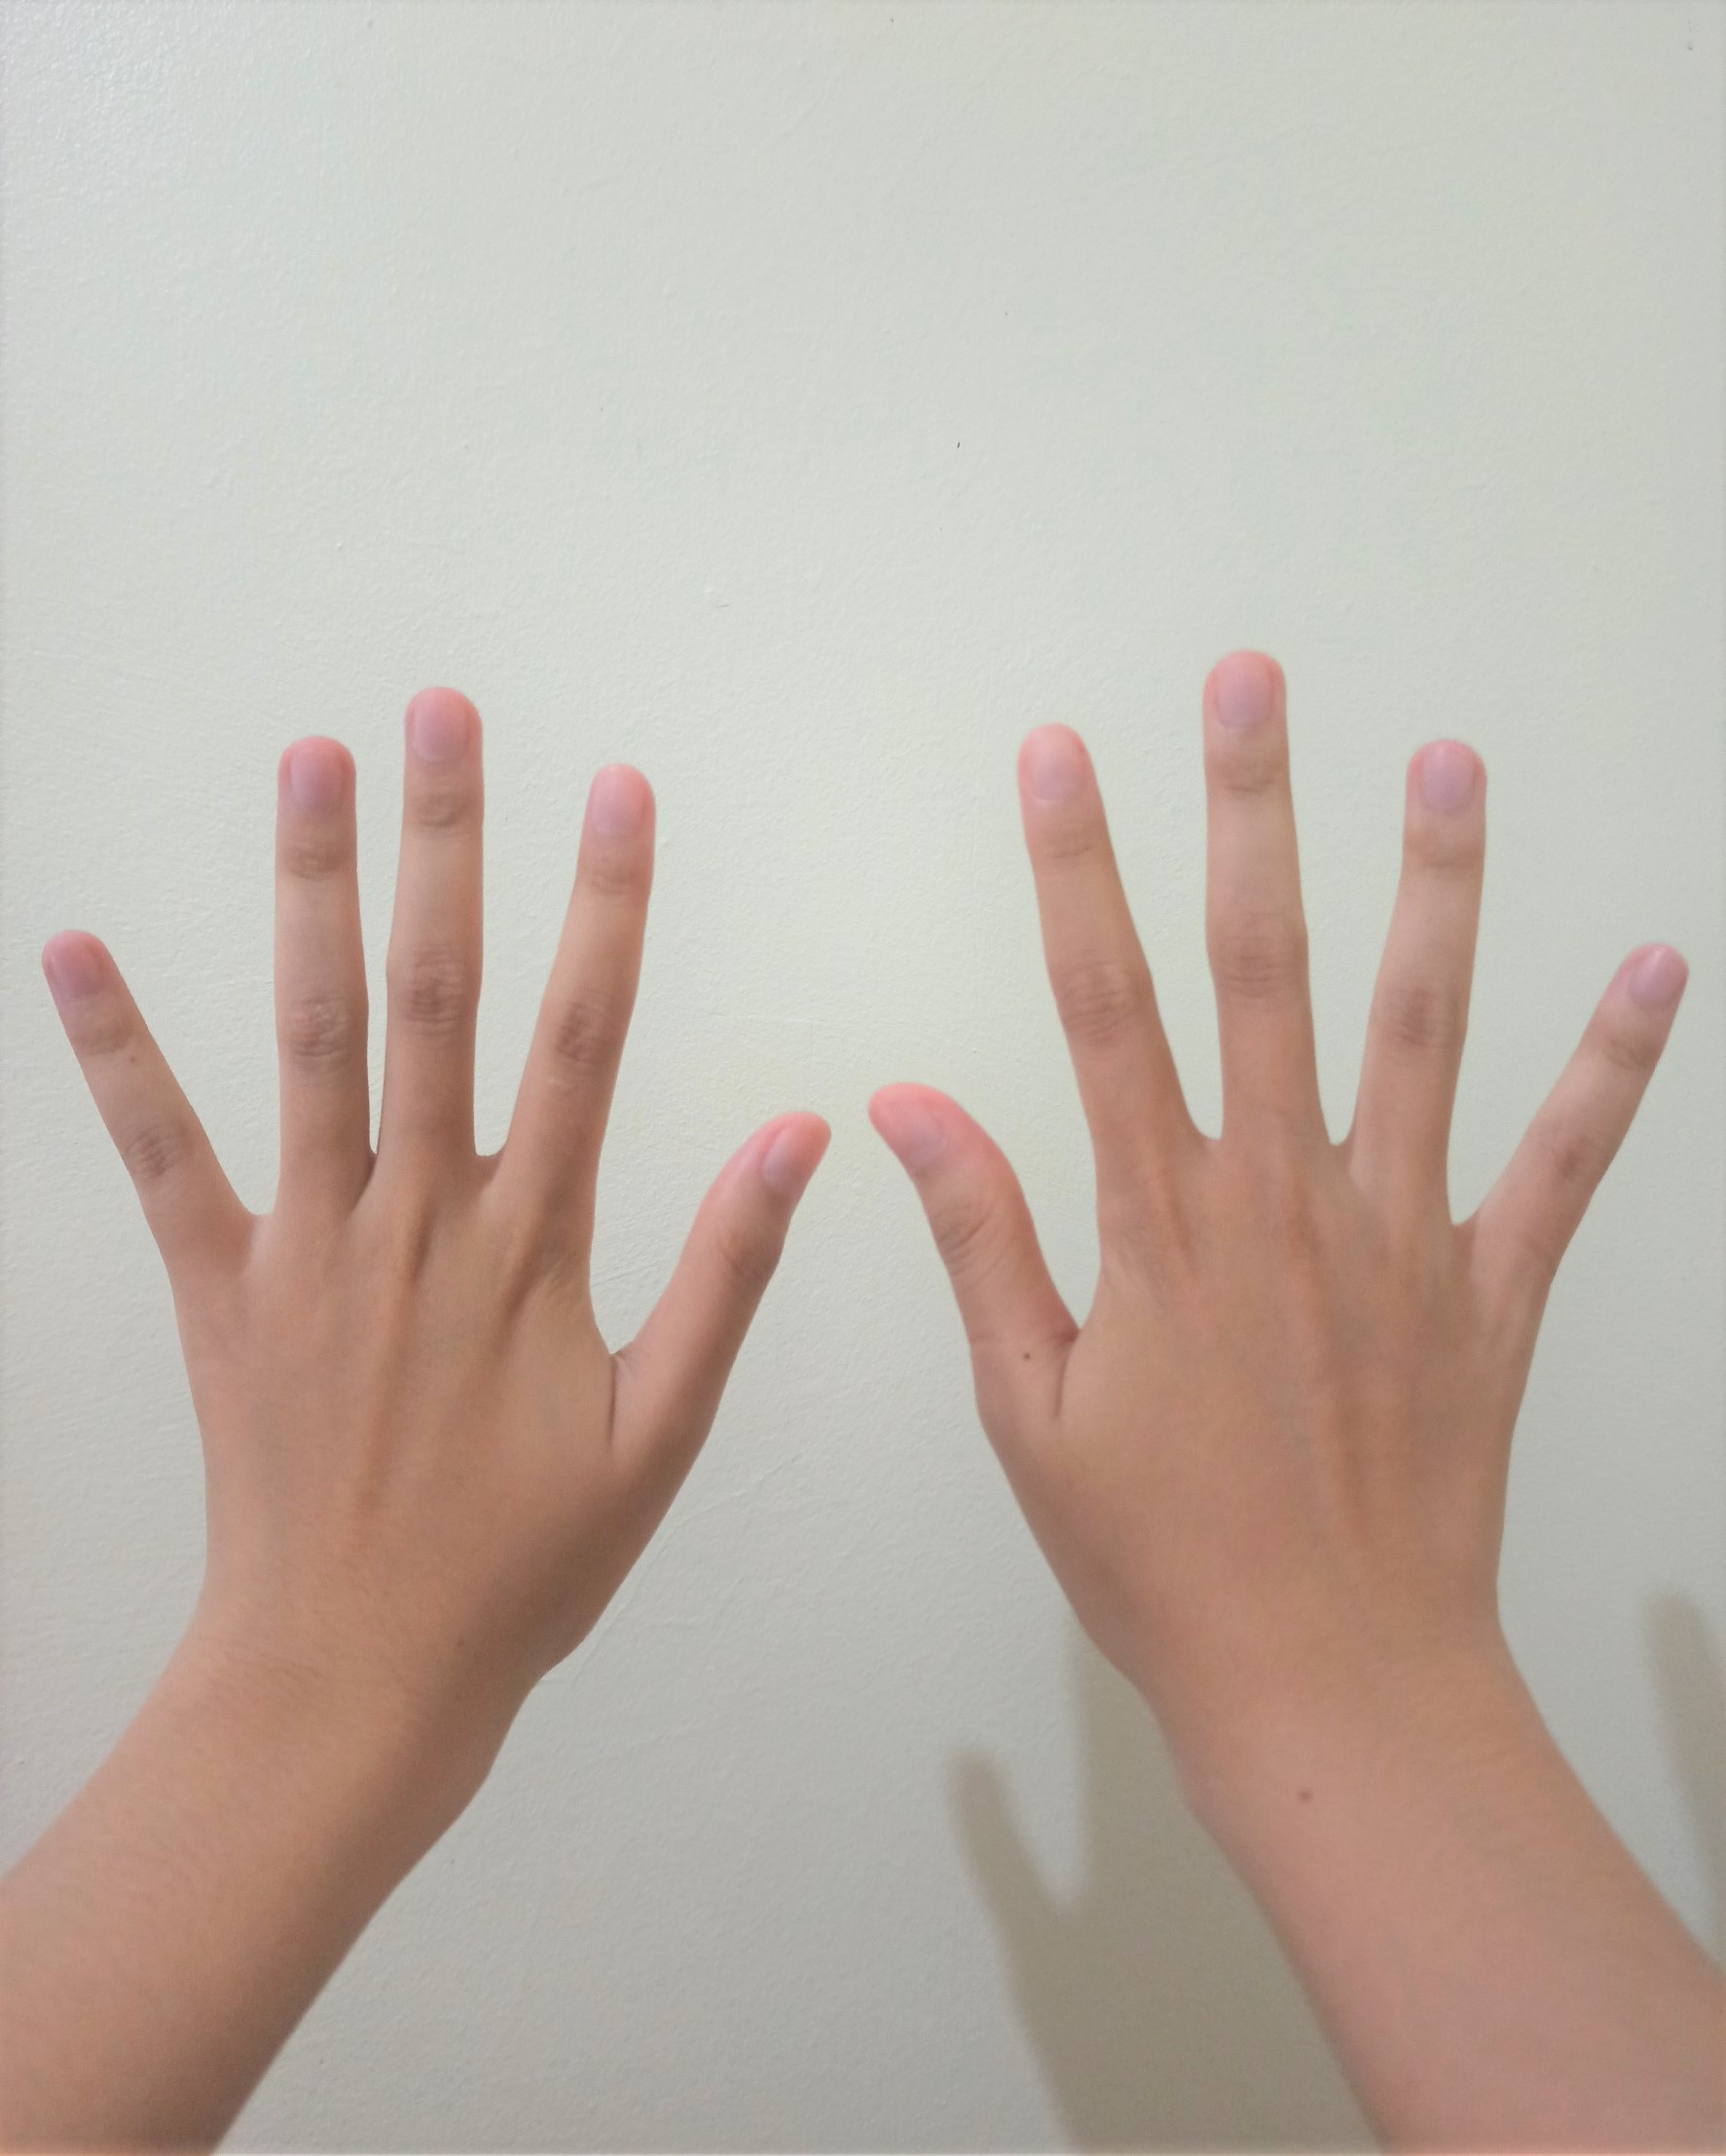
\includegraphics[width=\textwidth]{img/pola4.jpg}
			\caption{\label{fig:gs4}}
		\end{subfigure}
		\hspace{0.1em}
		\begin{subfigure}[t]{0.11\textwidth}
			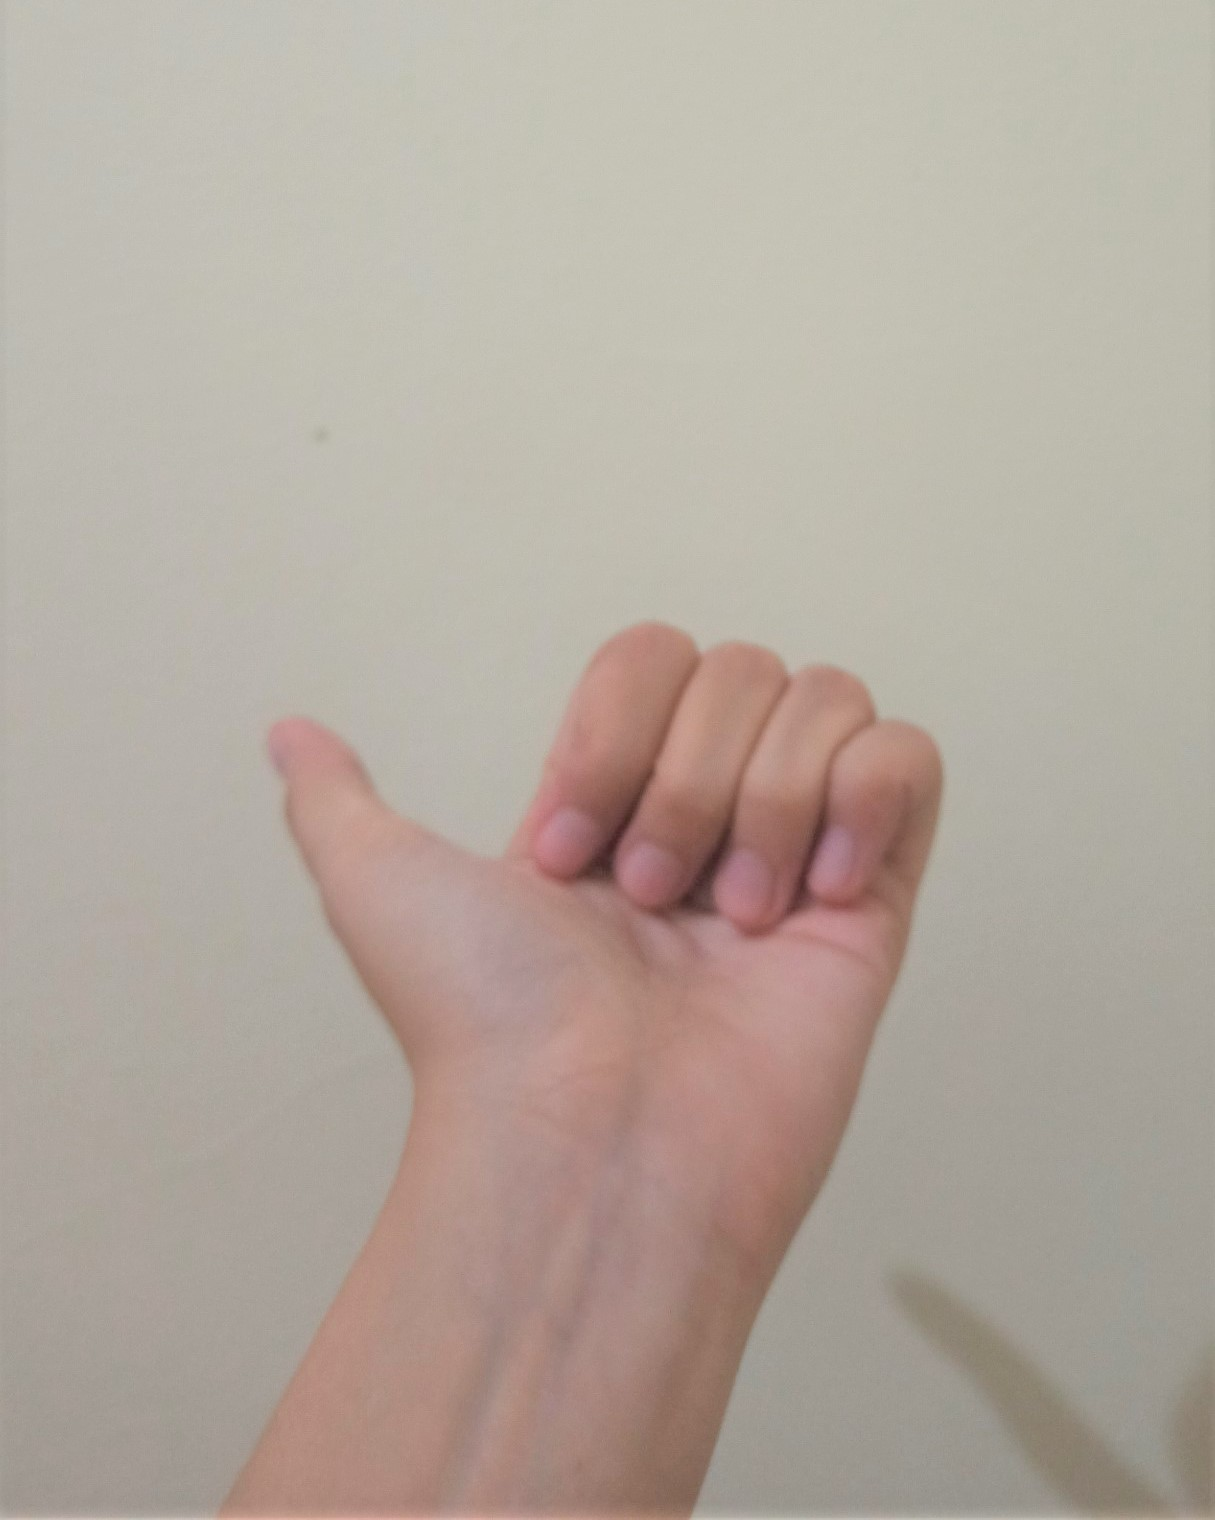
\includegraphics[width=\textwidth]{img/pola5a.jpg}
			\caption{\label{fig:gs5a}}
		\end{subfigure}
		\hspace{0.1em}
		\begin{subfigure}[t]{0.11\textwidth}
			\centering
			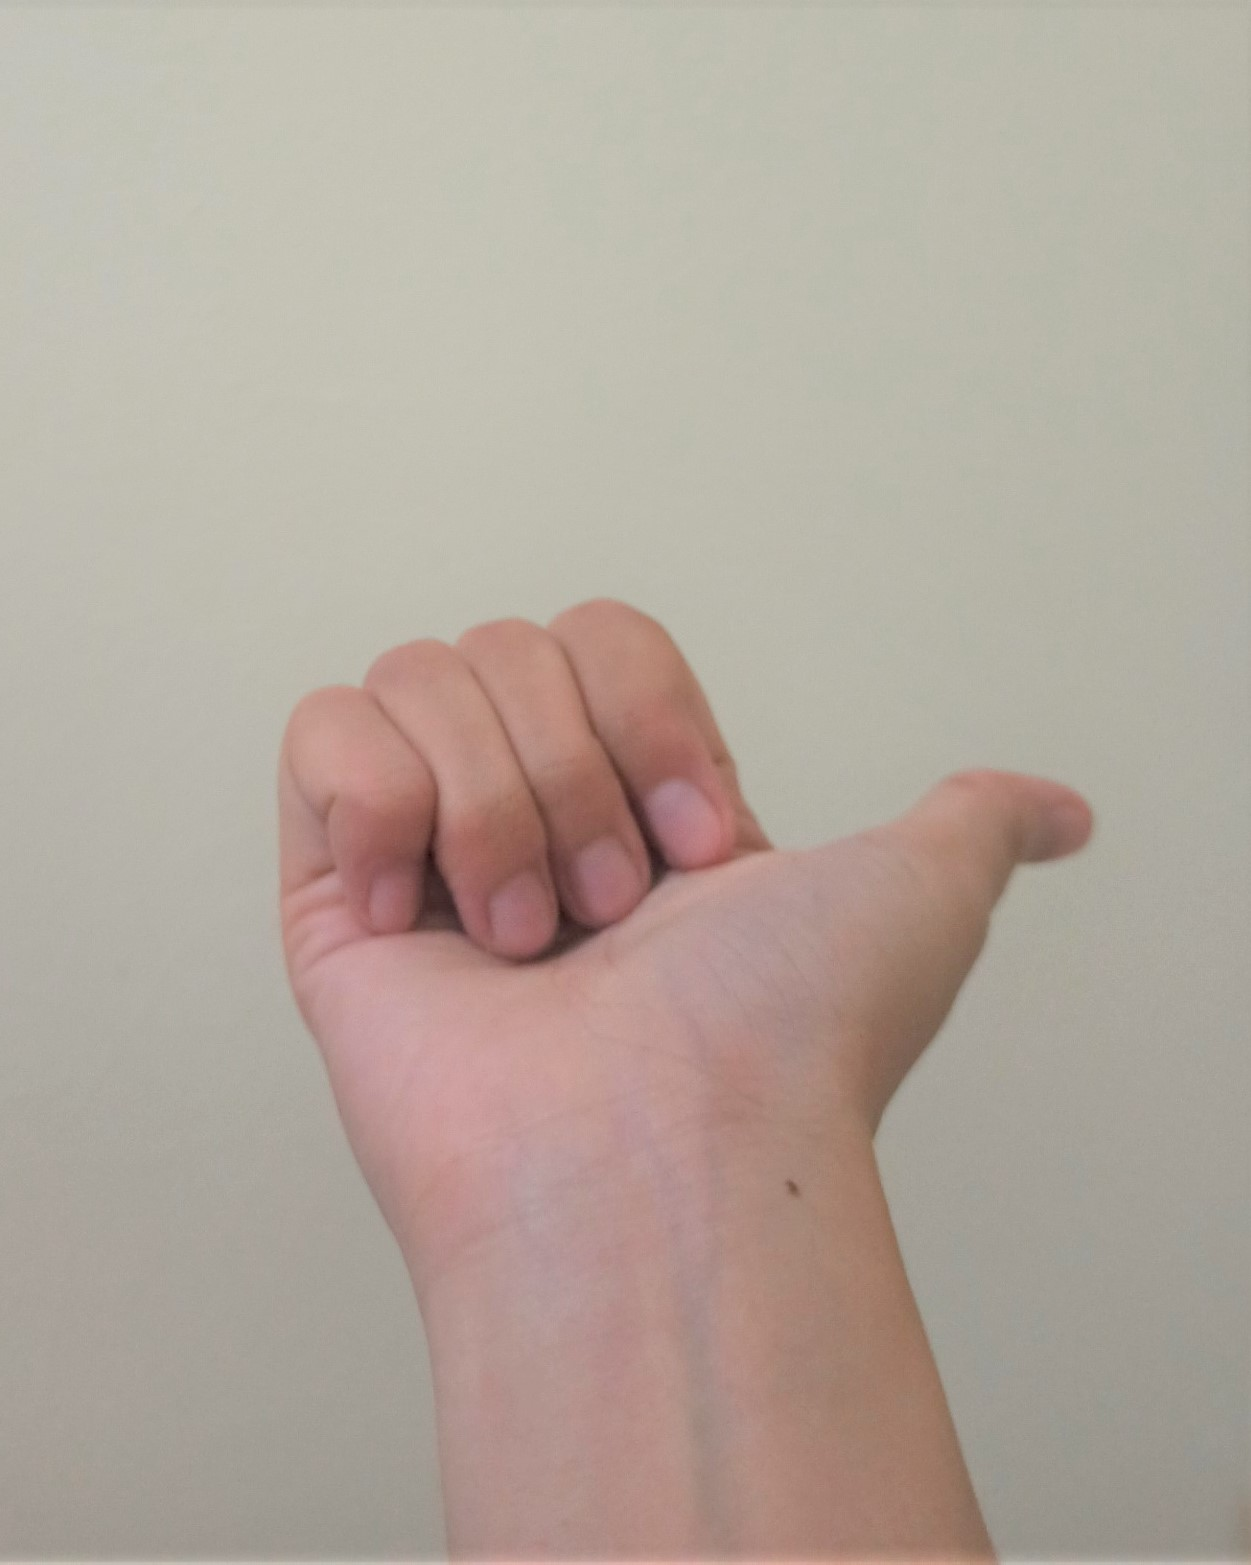
\includegraphics[width=\textwidth]{img/pola5b.jpg}
			\caption{\label{fig:gs5b}}
		\end{subfigure}
		\hspace{0.1em}
		\begin{subfigure}[t]{0.11\textwidth}
			\centering
			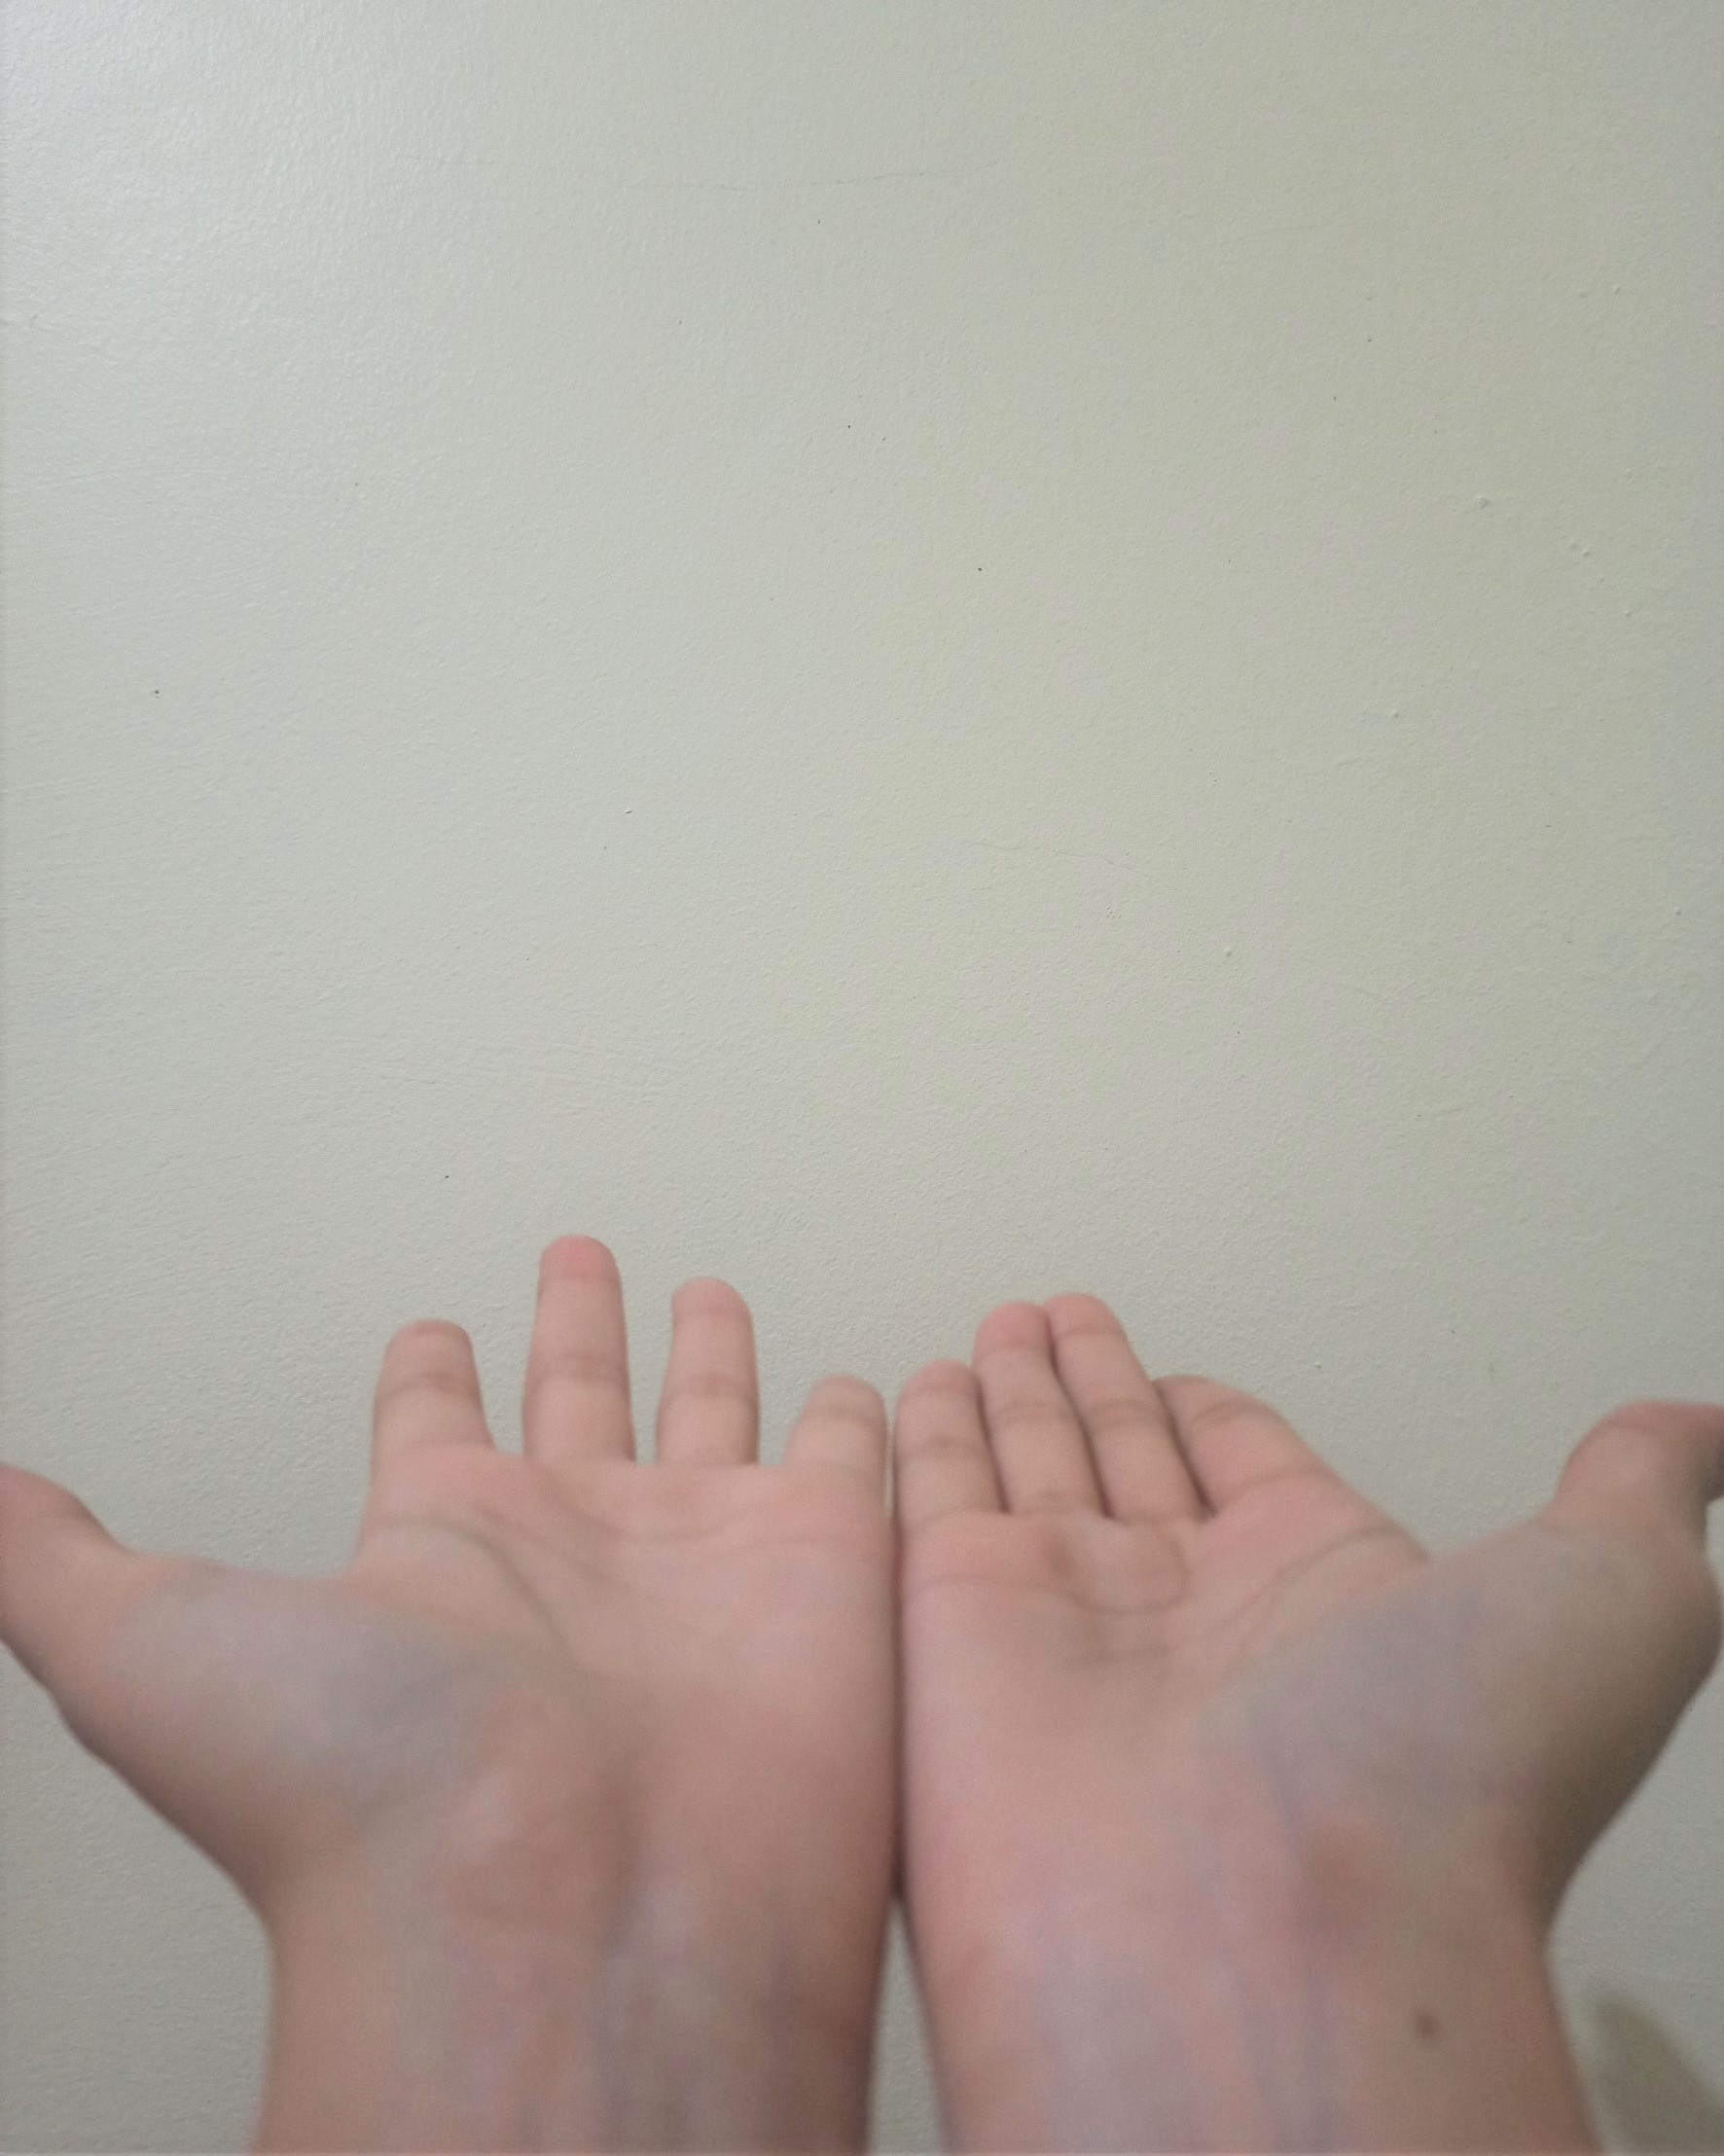
\includegraphics[width=\textwidth]{img/pola6.jpg}
			\caption{\label{fig:gs6}}
		\end{subfigure}
		\hspace{0.1em}
		\begin{subfigure}[t]{0.11\textwidth}
			\centering
			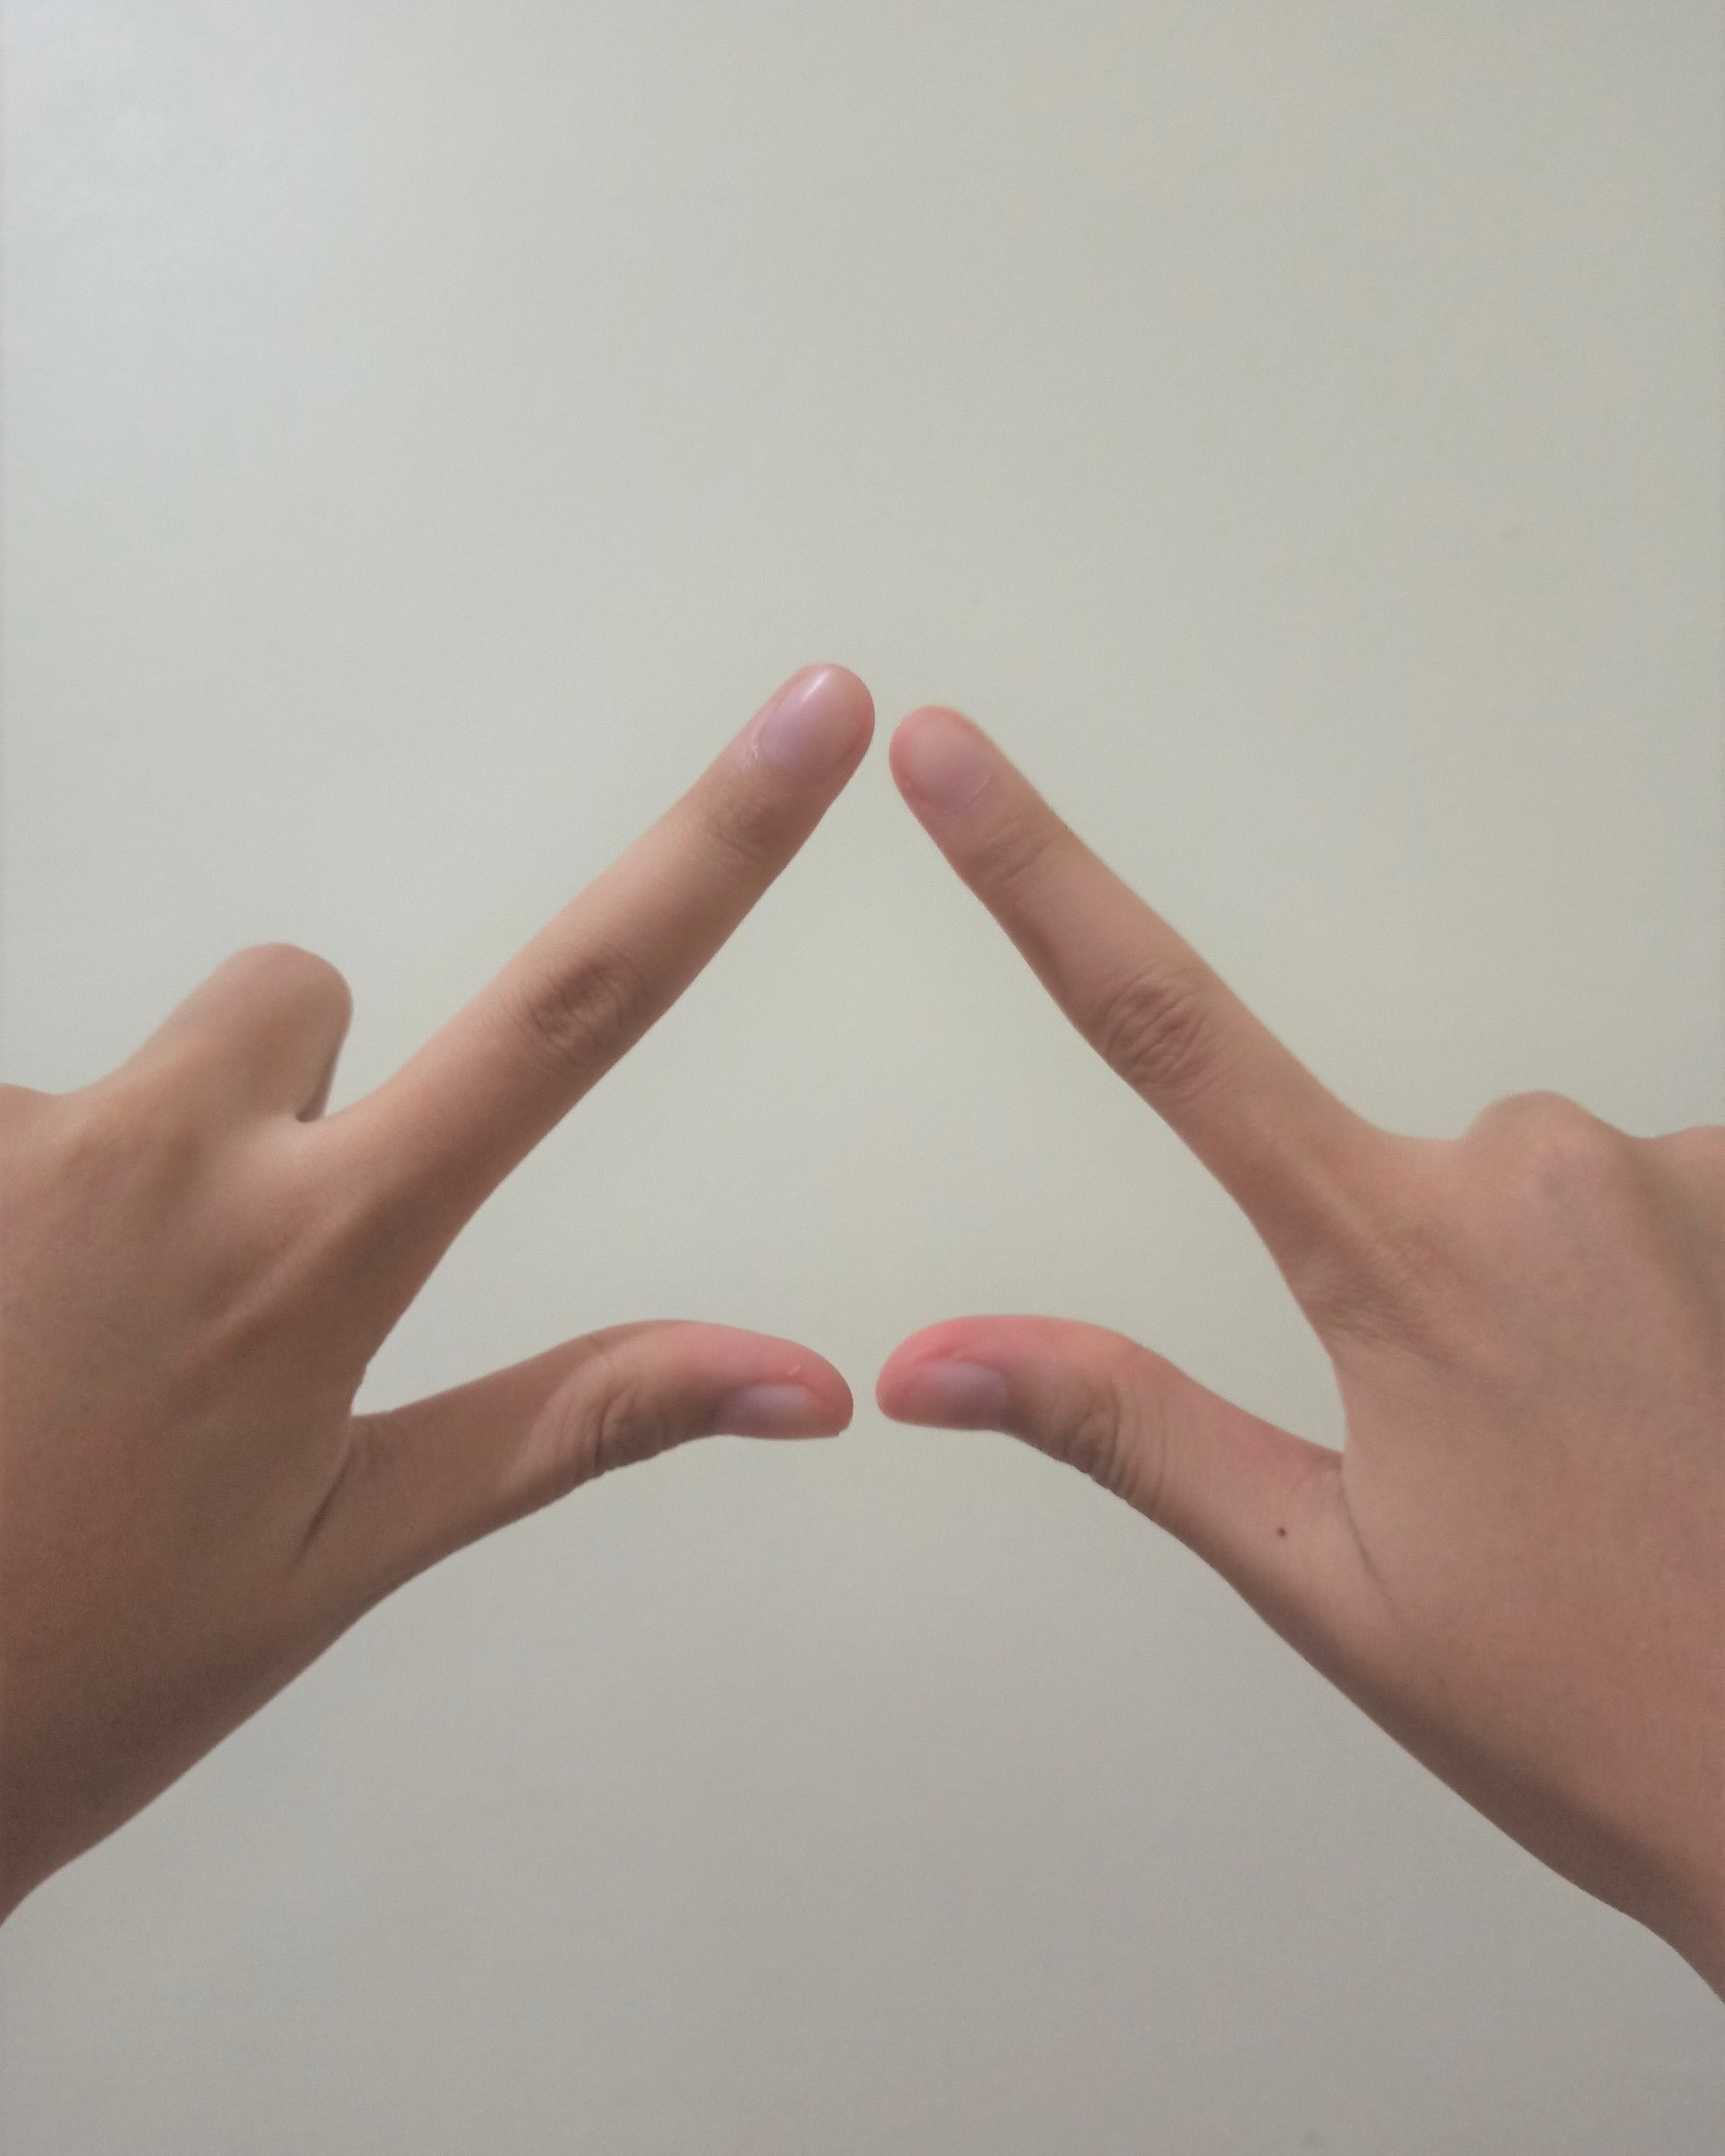
\includegraphics[width=\textwidth]{img/pola7.jpg}
			\caption{\label{fig:gs7}}
		\end{subfigure}
		\hspace{0.1em}
		\begin{subfigure}[t]{0.11\textwidth}
			\centering
			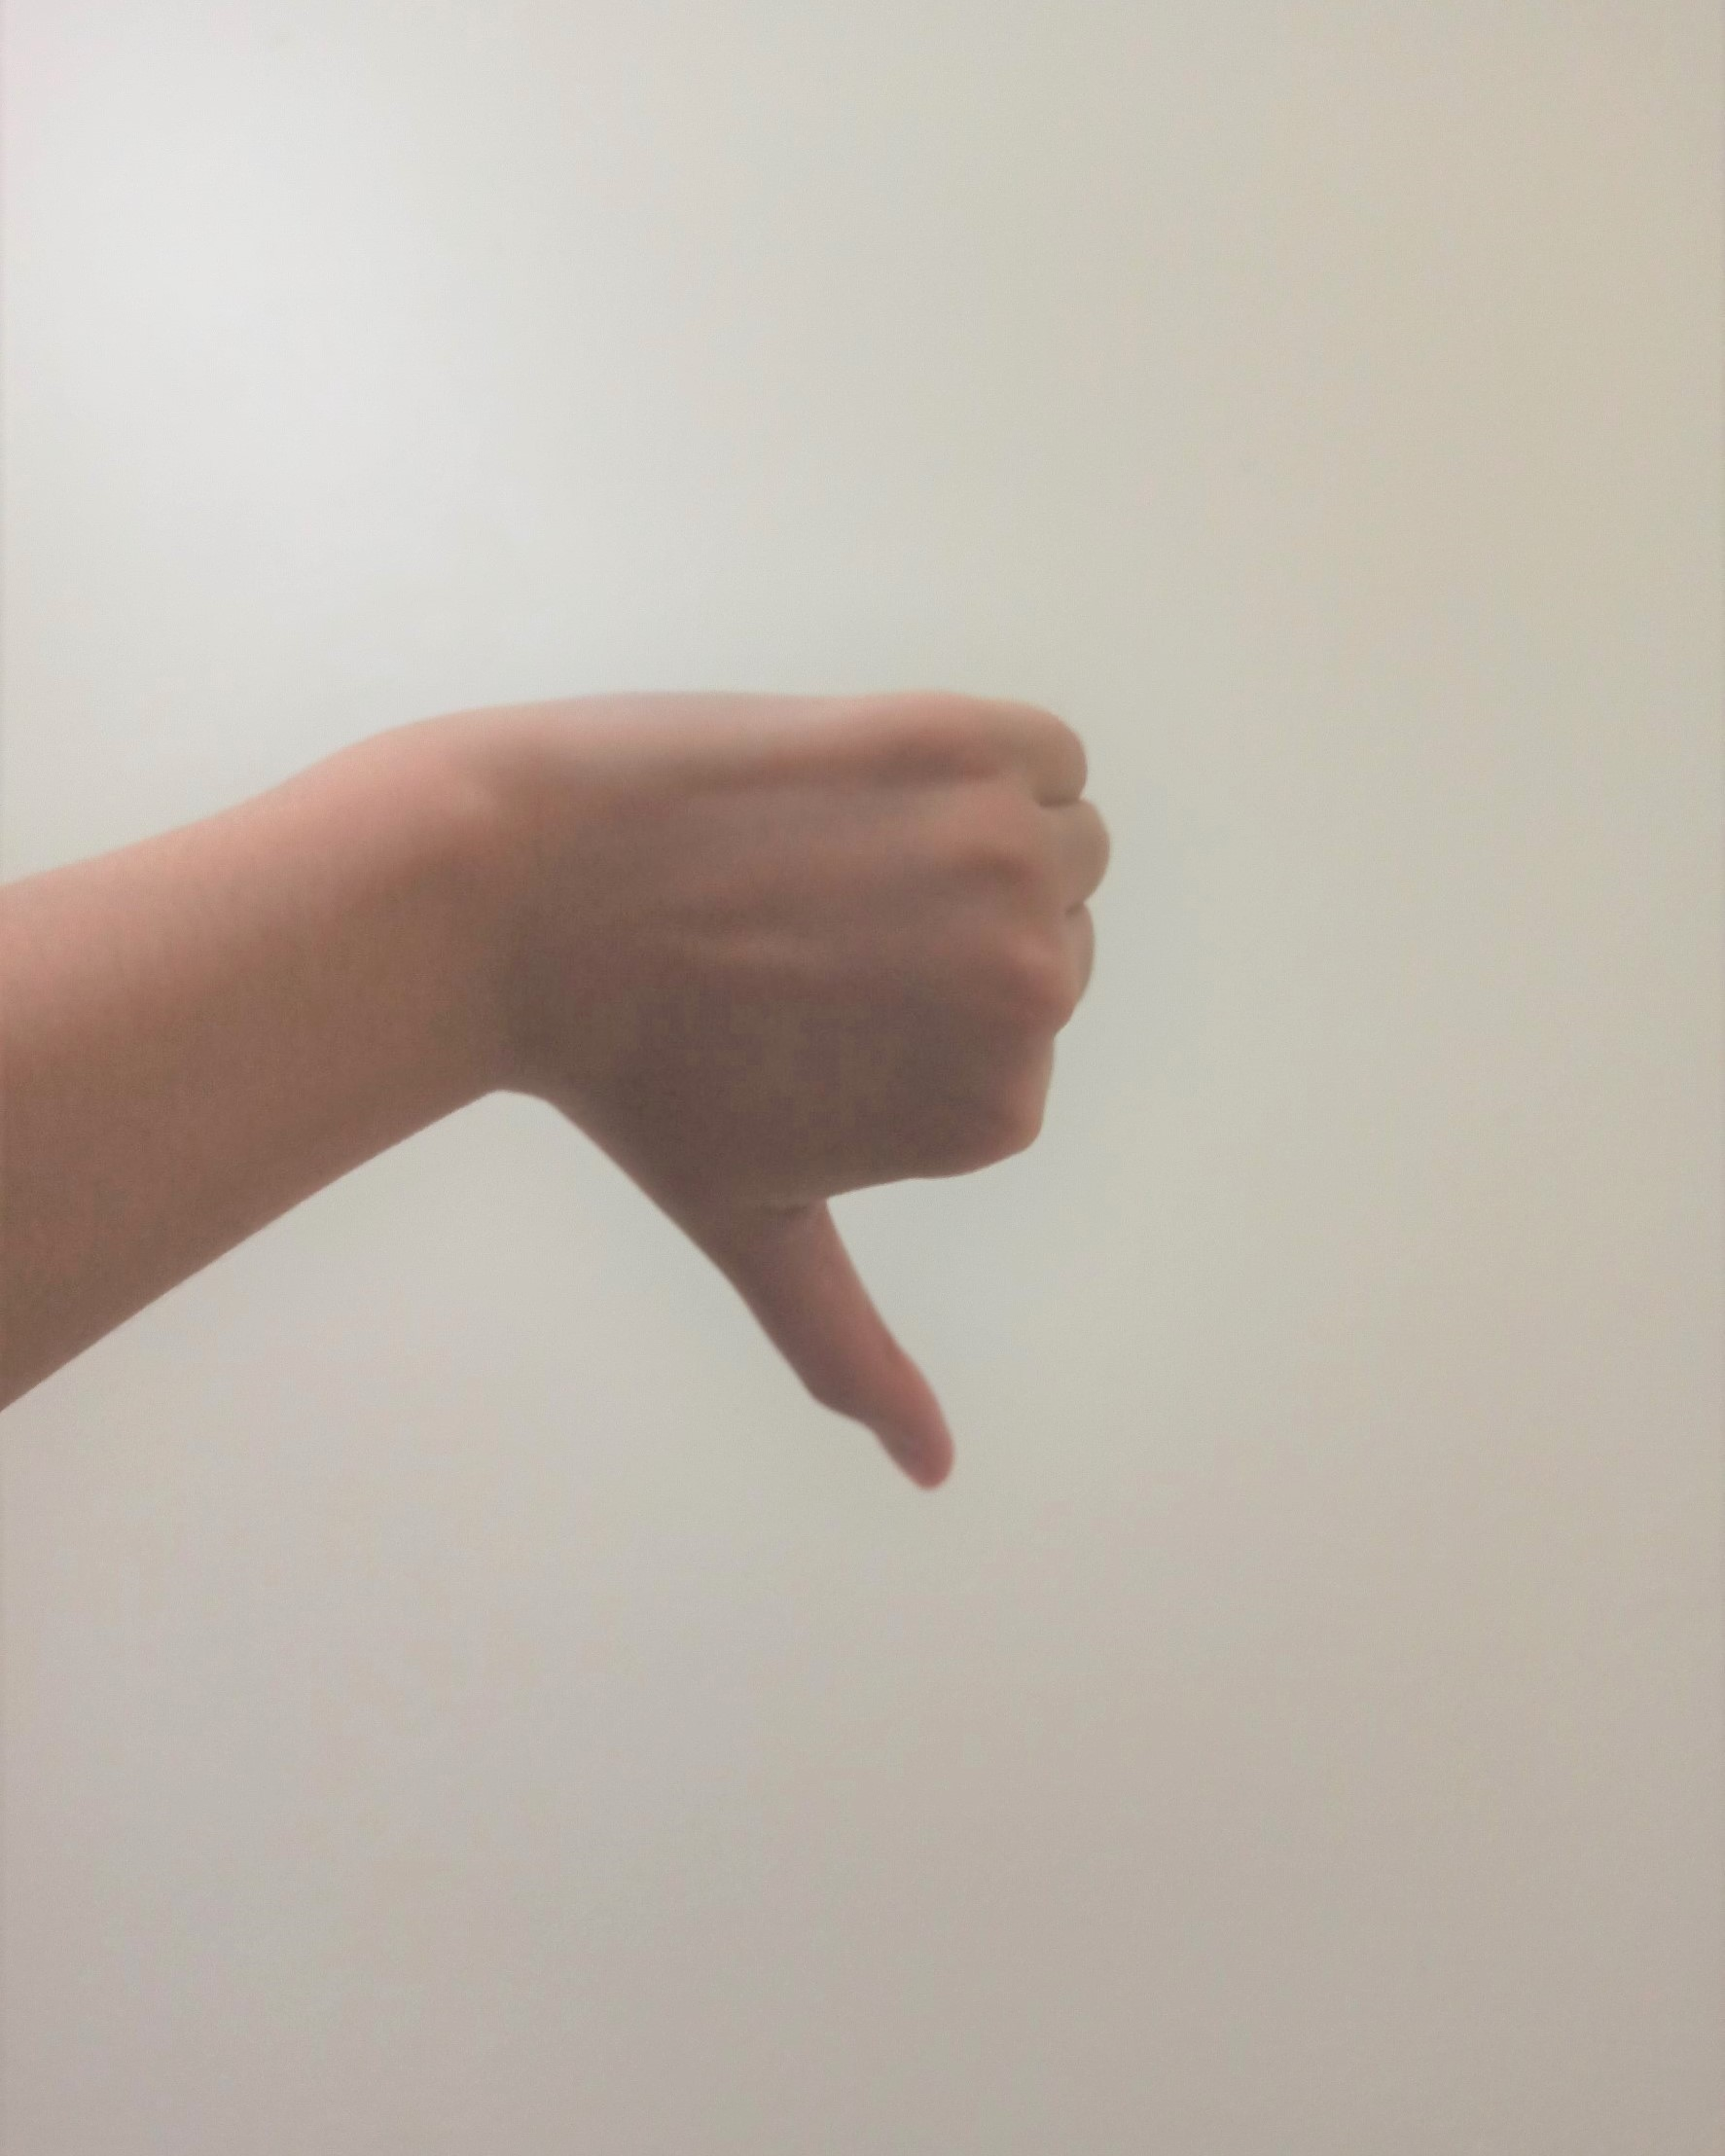
\includegraphics[width=\textwidth]{img/pola8a.jpg}
			\caption{\label{fig:gs8a}}
		\end{subfigure}
		\hspace{0.1em}
		\begin{subfigure}[t]{0.11\textwidth}
			\centering
			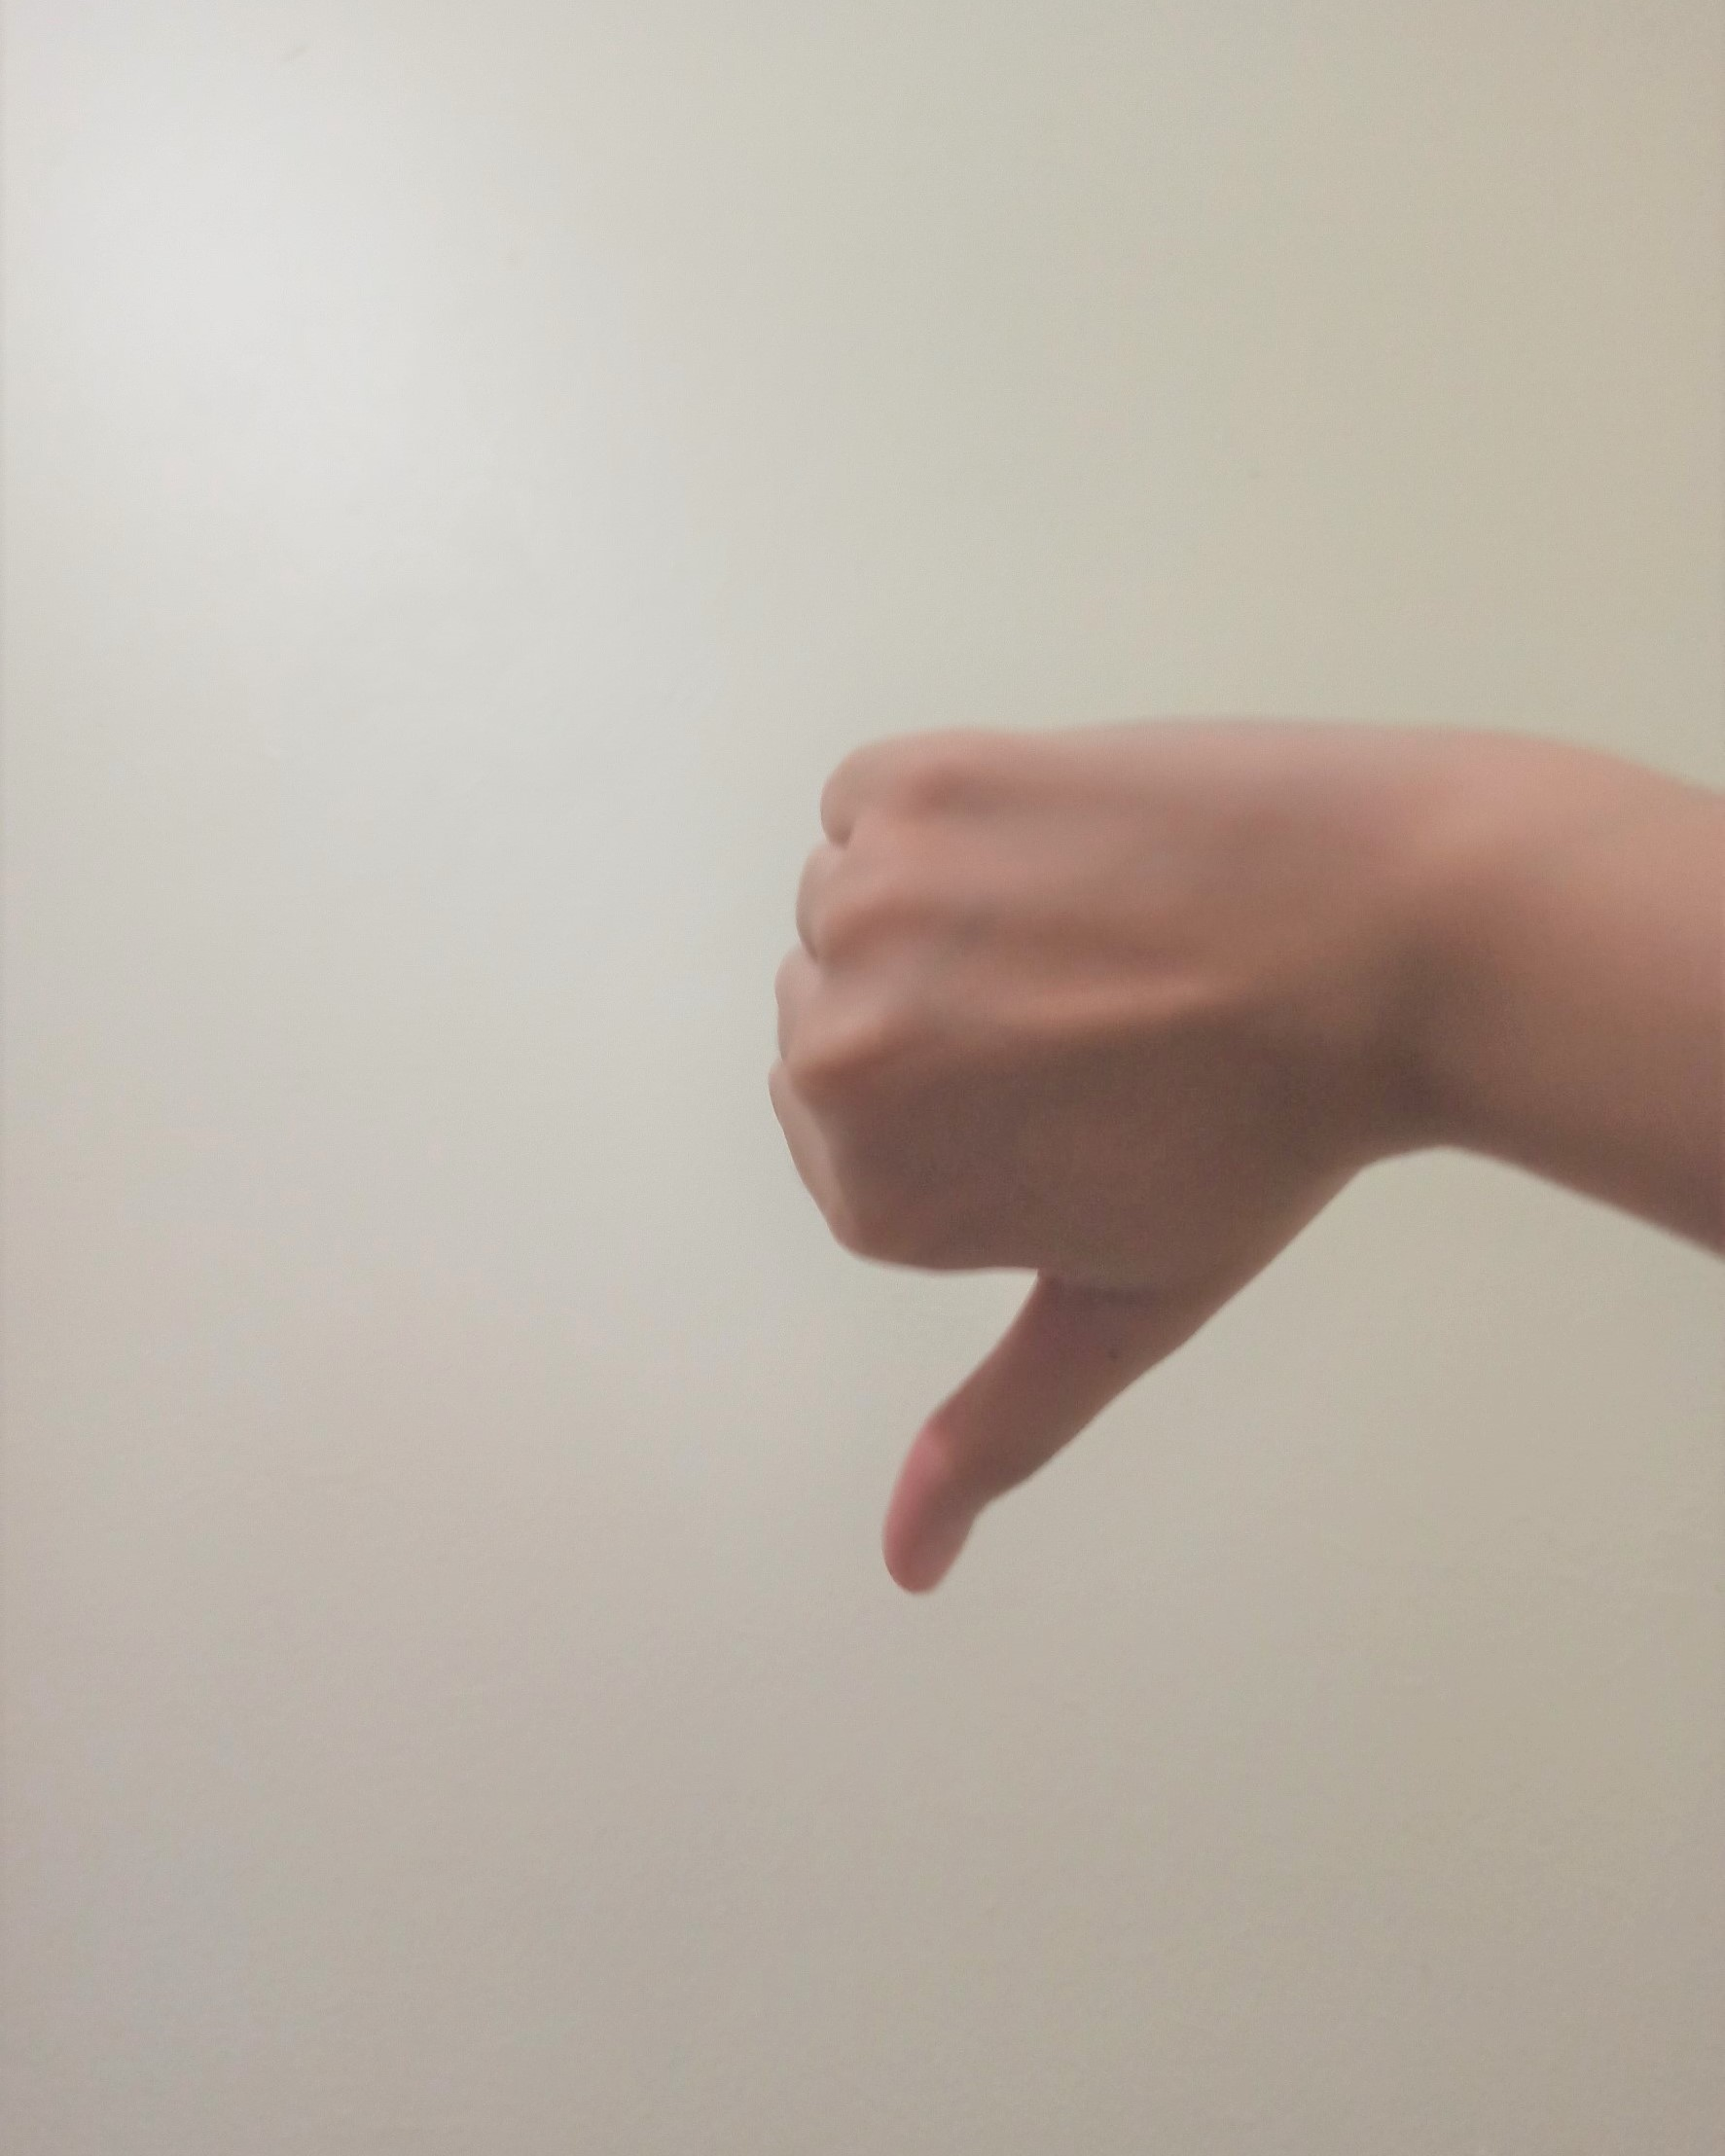
\includegraphics[width=\textwidth]{img/pola8b.jpg}
			\caption{\label{fig:gs8b}}
		\end{subfigure}
		\hspace{0.1em}
		\begin{subfigure}[t]{0.11\textwidth}
			\centering
			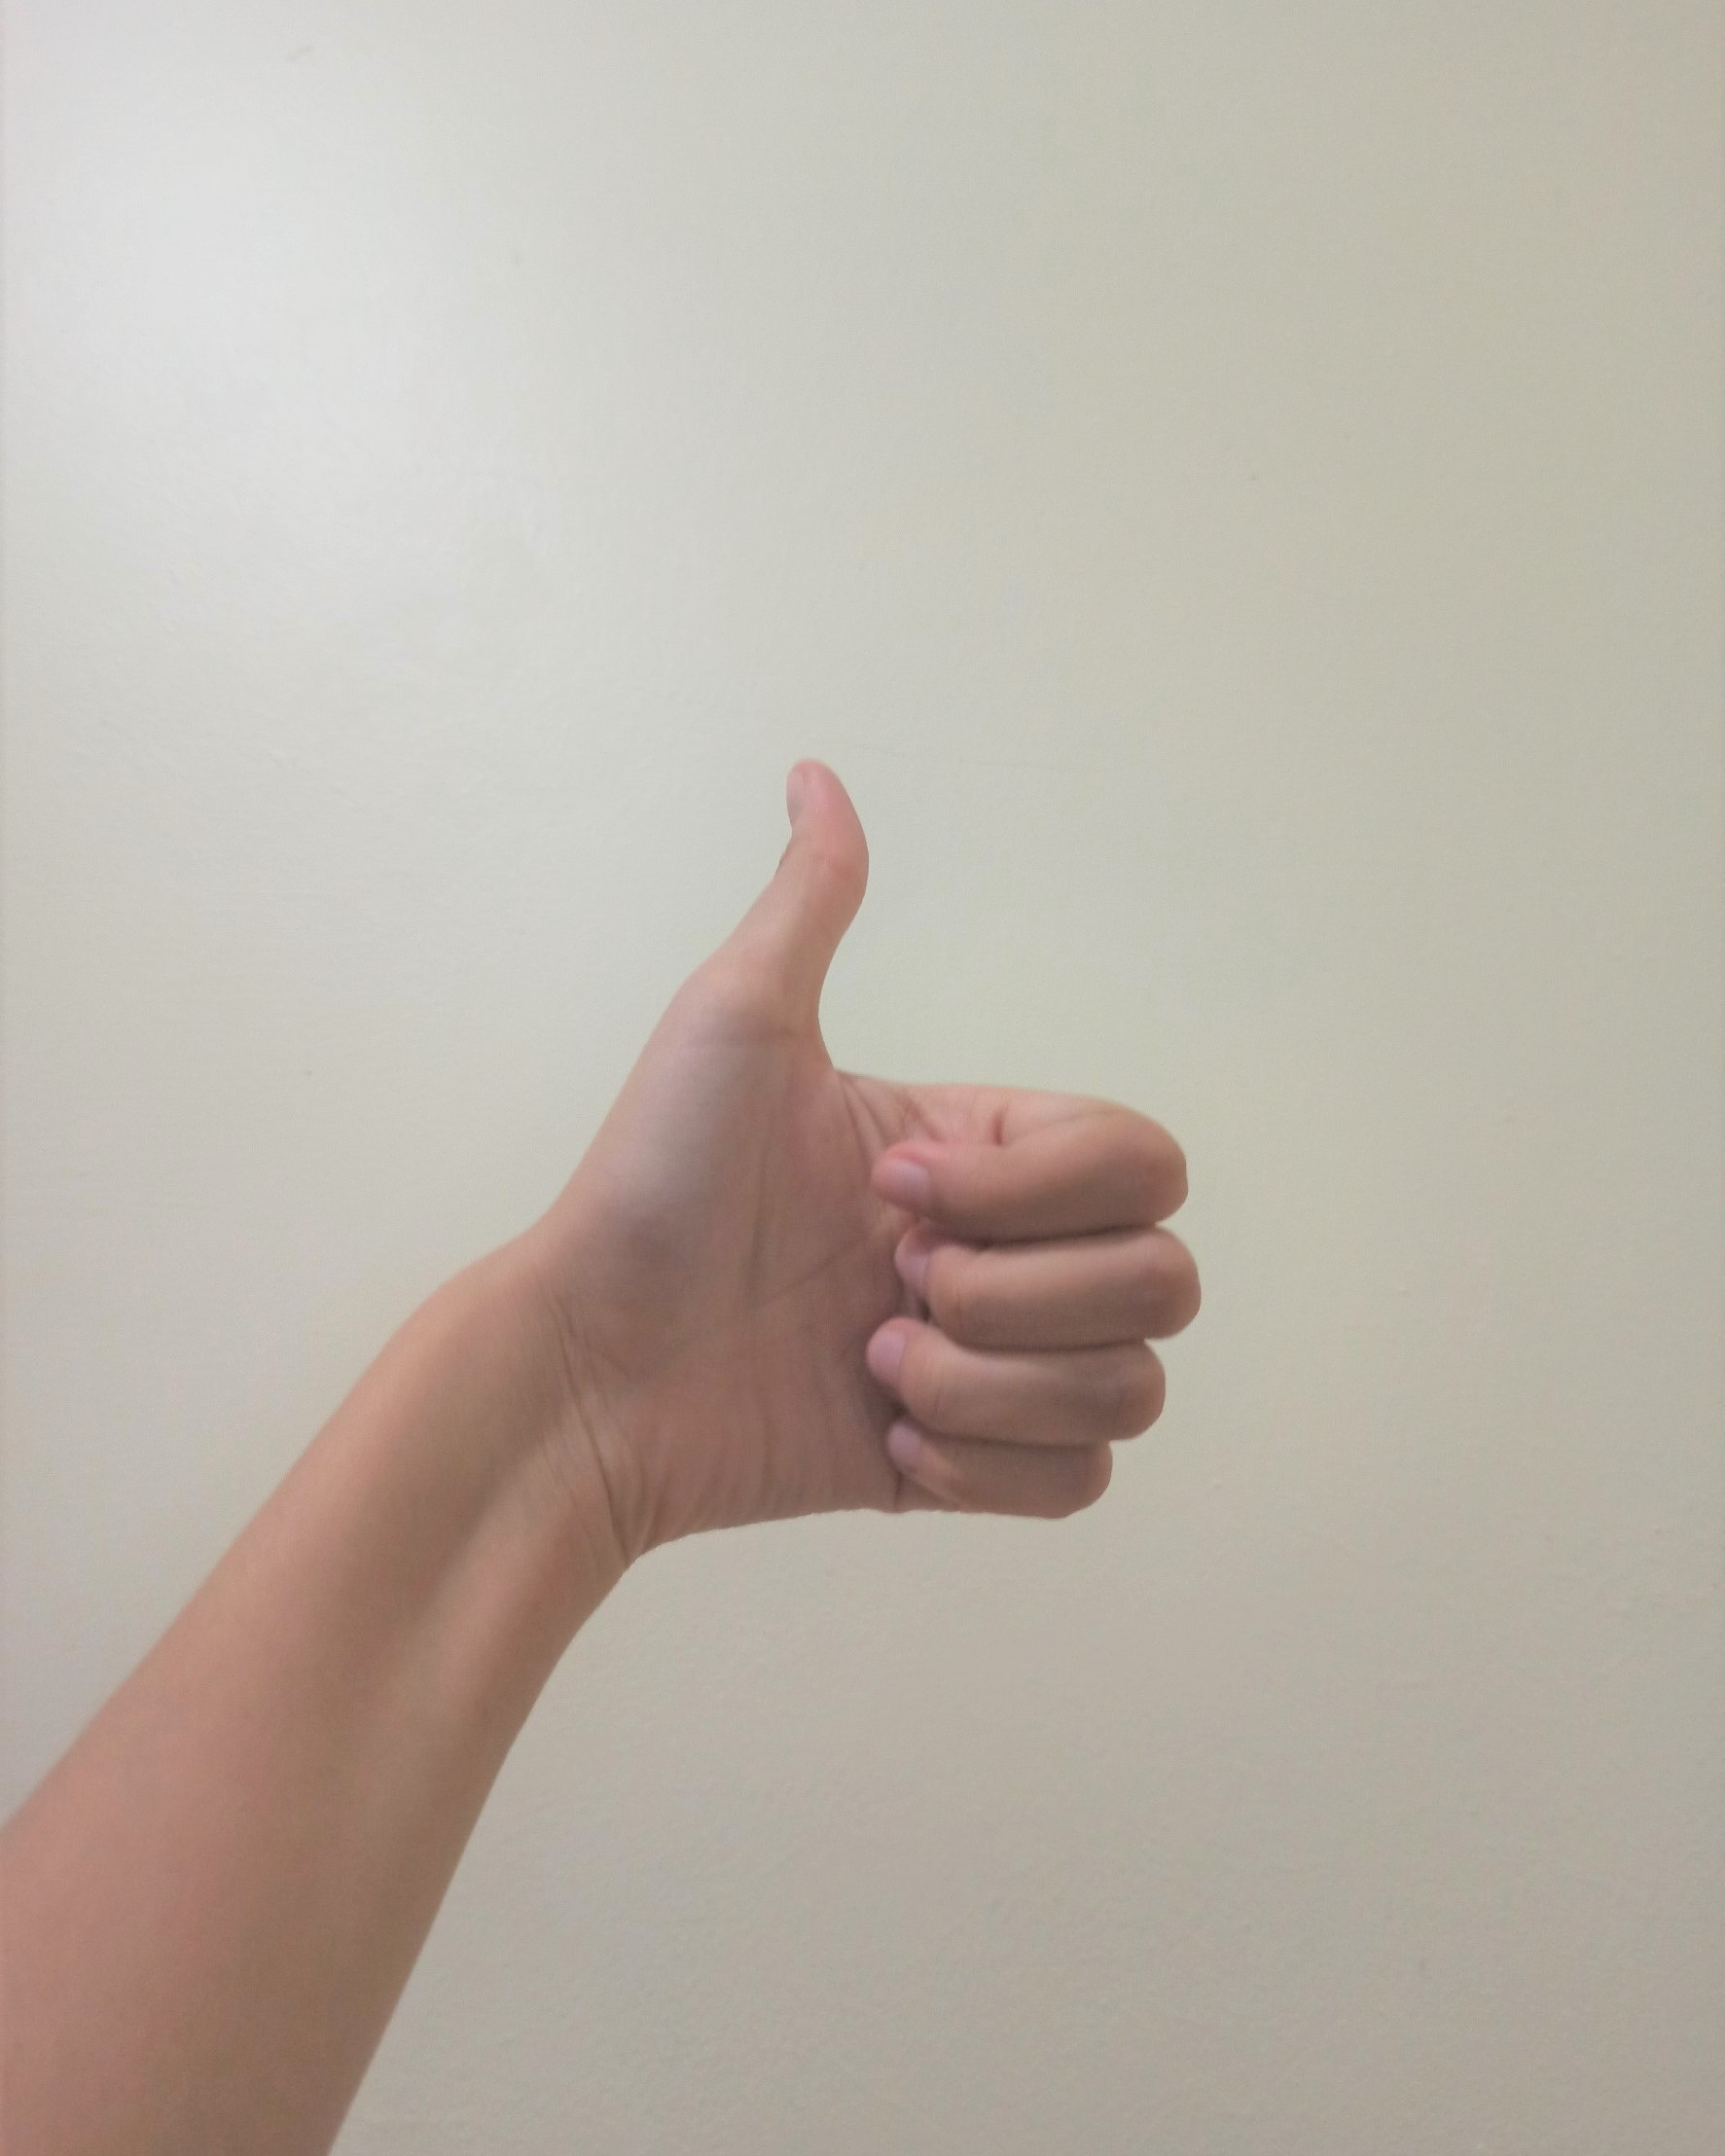
\includegraphics[width=\textwidth]{img/pola8c.jpg}
			\caption{\label{fig:gs8c}}
		\end{subfigure}
		\hspace{0.1em}
		\begin{subfigure}[t]{0.11\textwidth}
			\centering
			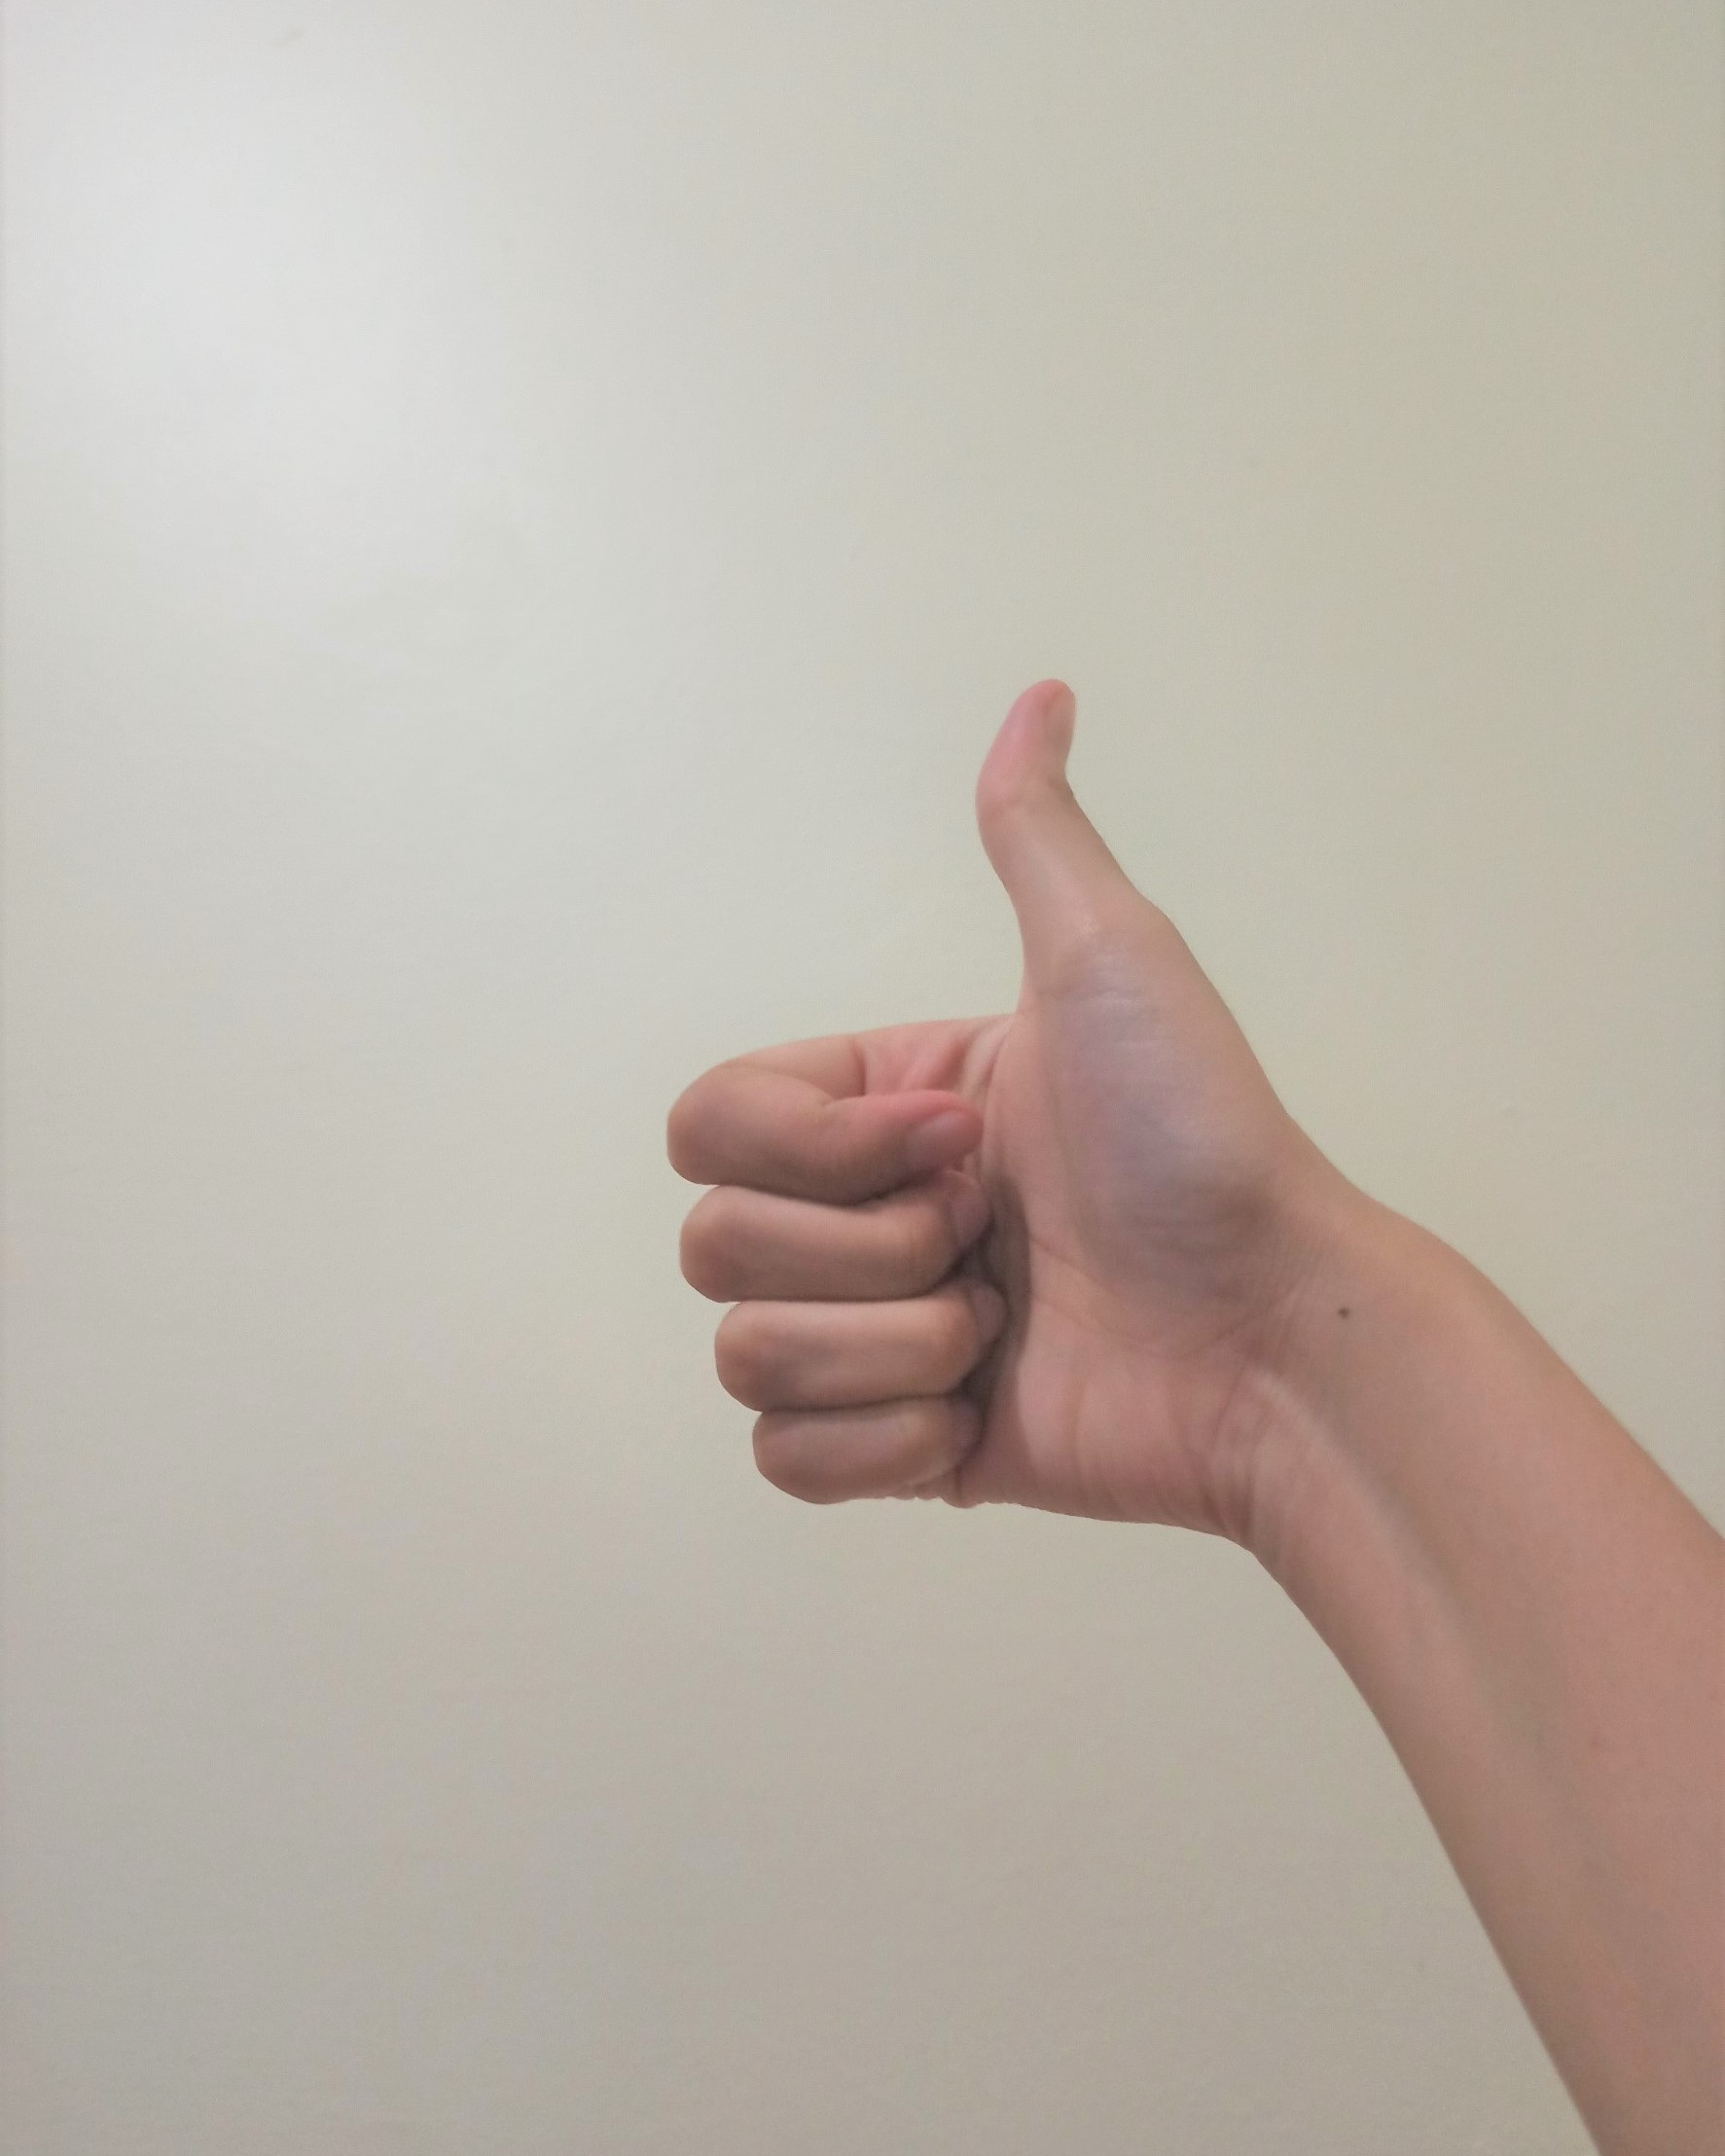
\includegraphics[width=\textwidth]{img/pola8d.jpg}
			\caption{\label{fig:gs8d}}
		\end{subfigure}
		\end{center}
		\vspace{-1ex}
		\caption{Hand gestures on the interaction system.}
		\label{fig:gestur_interaksi}
	\end{figure}
	\vspace{-2ex}
	
	\subsubsection{Reset to Default Algorithm }
		Reset to default is a feature that returns an object at its original position, rotation and size with \ref{fig:gs4} gesture. This feature allows users to see objects as a whole automatically without having to adjust them one by one (without moving, rotating, or zooming manually).

	\subsubsection{Object Substitution Algorithm}
		The user can select both the before and after objects of the currently displayed object. The hologram object and the information conveyed can be changed through the \ref{fig:gs5a} and \ref{fig:gs5b} gestures without selecting a button on the information monitor.

	\subsubsection{Displays the Help Menu Algorithm}
		When in Main Scene, the user can display the Help menu to open the device's use of the form of viewing variations of gestures that are owned and layout information object information on the information monitor. Users can access this feature via \ref{fig:gs6} gesture without selecting a button on the information monitor.

	\subsubsection{Display Menu Algorithm}
		This feature is similar to the Algorithm Display Menu Help, only the menu that is displayed is the Main Menu or can also be known to exit the Main Scene. The gesture in this algorithm is similar to Reset to Default Algorithm (figure \ref{fig:gs4}), the difference is the thumb and index finger which are close together (figure \ref{fig:gs7}) can be determined through the equation \ref{eqn:position_target}.

	\subsubsection{Algorithm Cancel or Select Options }
		When the Main Scene is run, the user can display the Help menu and Main Menu which have several buttons. Users can also access the button using the corresponding gestures. The button to deselect (back and cancel) can be accessed using the \ref{fig:gs8a} and \ref{fig:gs8b} gestures. While the button to approve the selection (OK) can be accessed using the gesture \ref{fig:gs8c} and \ref{fig:gs8d}.


\section{TESTING AND RESULTS}
	\subsection{Hologram Projection Testing} 
		\vspace{-2ex}
		\begin{figure}[h]
			\begin{center}
				\begin{subfigure}[t]{0.11\textwidth}
					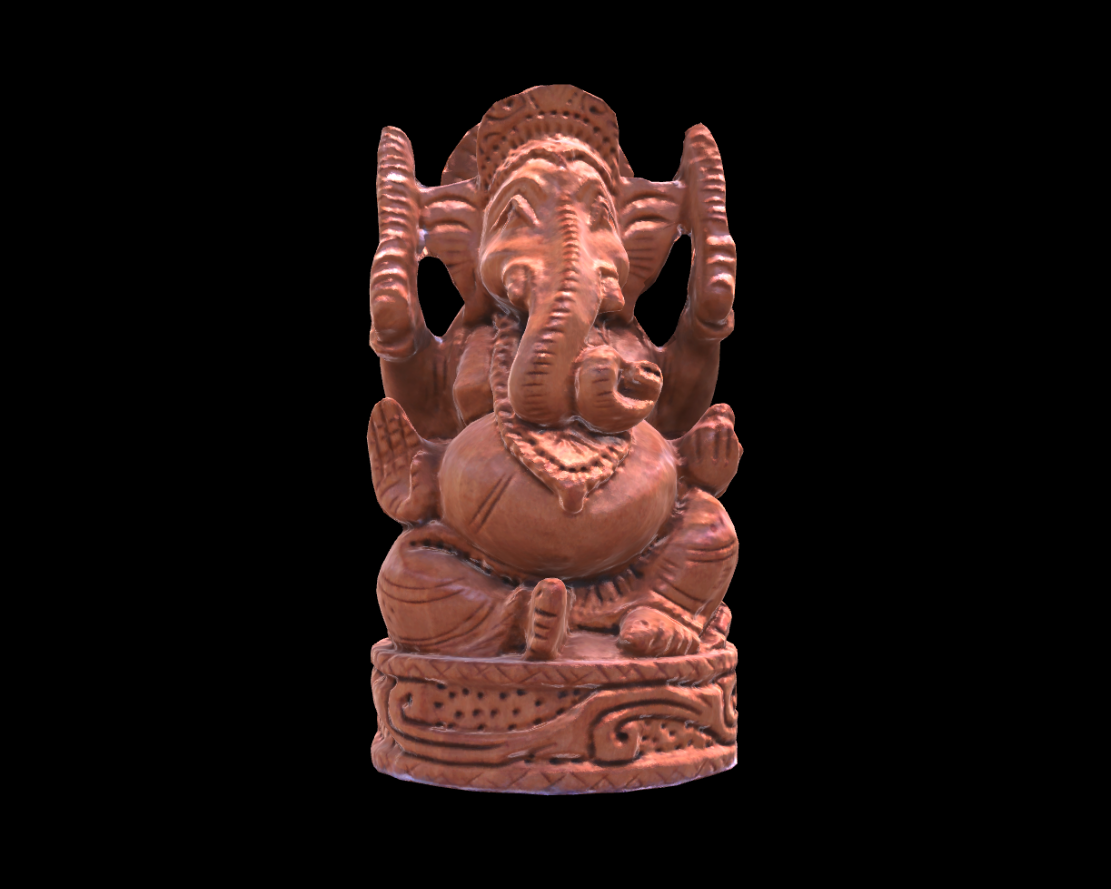
\includegraphics[width=\textwidth]{img/ilusi1.png}
					\caption{\label{fig:ilusi1}}
				\end{subfigure}
				\hspace{0.05em}
				\begin{subfigure}[t]{0.11\textwidth}
					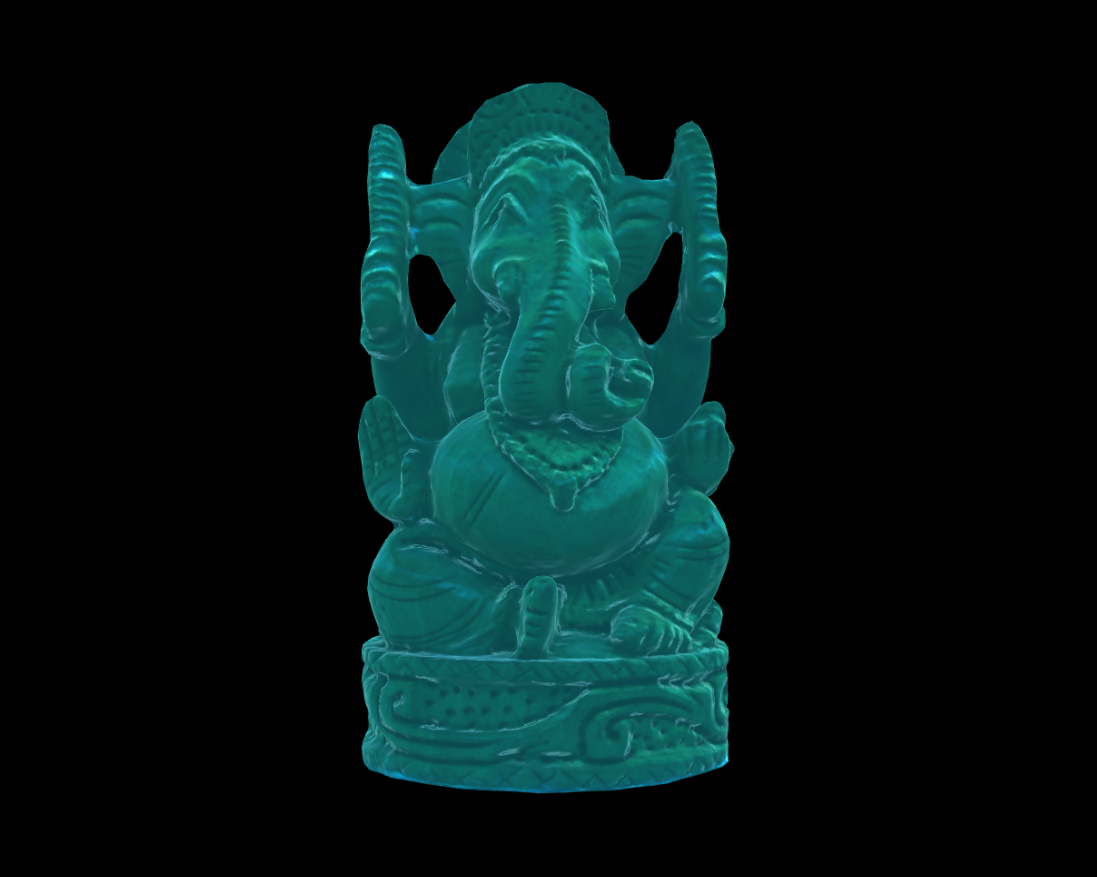
\includegraphics[width=\textwidth]{img/ilusi2.png}
					\caption{\label{fig:ilusi2}}
				\end{subfigure}
				\hspace{0.05em}
				\begin{subfigure}[t]{0.11\textwidth}
					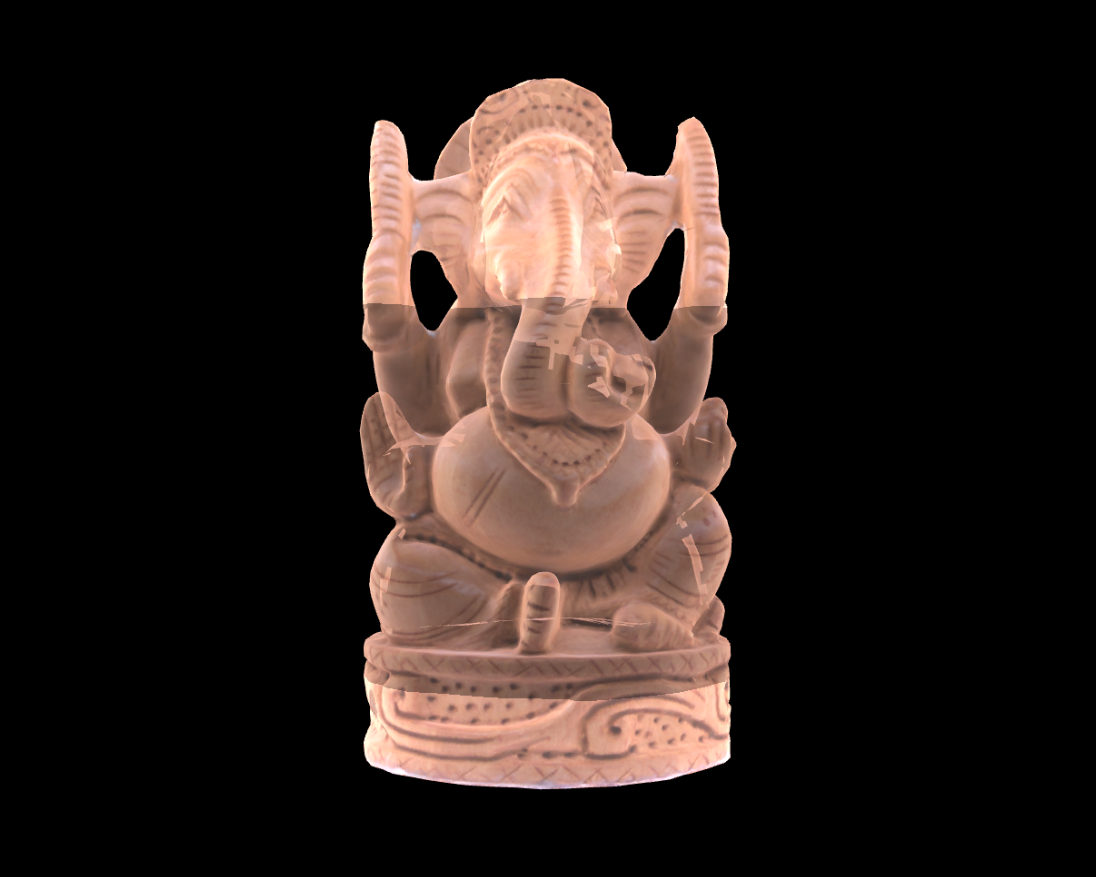
\includegraphics[width=\textwidth]{img/ilusi3.png}
					\caption{\label{fig:ilusi3}}
				\end{subfigure}
				\hspace{0.05em}
				\begin{subfigure}[t]{0.11\textwidth}
					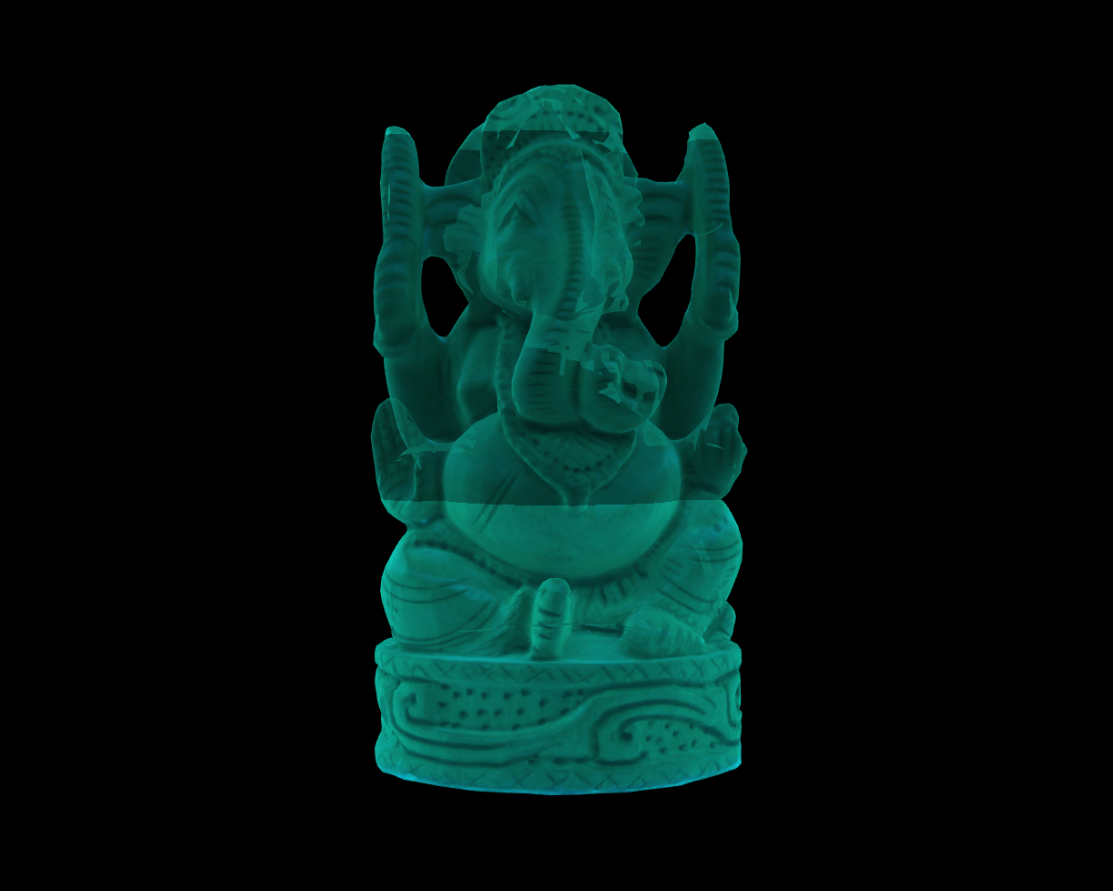
\includegraphics[width=\textwidth]{img/ilusi4.png}
					\caption{\label{fig:ilusi4}}
				\end{subfigure}
			\end{center}
			\vspace{-1ex}
			\caption{Setting for holographic effects.}
			\label{fig:sb_p1}
		\end{figure}
		\vspace{-2ex}
		
		This test aims to determine the effect of which holographic illusion is suitable for 3D objects to be projected on the holographic pyramid. Testing the presentation of the hologram object is done by giving 4 different settings to each 3D object and analyzing the results of the projection according to the figure \ref{fig:sb_p1}. The test is calculated by giving a value for each hologram treatment for each object based on the level of firmness of the holographic object displayed, where Very Good (VG) = 3 points, Good (G) = 2 points, Not Good (NG) = 1 point. The test results are listed in the table \ref{tab:hasil_penyajian}.
		\vspace{-1ex}
		\begin{table}[h]
			\caption{The results of the hologram presentation test.}
			\label{tab:hasil_penyajian}
			\vspace{-2ex}
			\begin{center}
				\begin{tabular}{|C{0.3cm}|L{2cm}|C{0.7cm}|C{0.7cm}|C{0.7cm}|C{0.7cm}|}
					\hline
					\multirow{2}{*}{\textbf{No}} & \multicolumn{1}{c|}{\multirow{2}{*}{\textbf{Object}}} & \multicolumn{4}{c|}{\textbf{Hologram Effect (point)}} \\ \cline{3-6}
					& \multicolumn{1}{c|}{}& \multicolumn{1}{c|}{\textbf{A}} & \multicolumn{1}{c|}{\textbf{B}} & \multicolumn{1}{c|}{\textbf{C}} & \multicolumn{1}{c|}{\textbf{D}} \\ \hline
					1.&Hand Axe		& 3 & 1 & 2 & 1 \\ \hline
					2.&Primeval Axe	& 2 & 1 & 3 & 1 \\ \hline
					3.&Buddha Statue	& 2 & 1 & 3 & 2 \\ \hline
					4.&Ganesha Statue	& 2 & 1 & 3 & 3 \\ \hline
					5.&Brass Lamp		& 2 & 1 & 3 & 2 \\ \hline
					6.&Ceramic Pot	& 3 & 1 & 3 & 1 \\ \hline
					7.&Typewriter		& 3 & 1 & 3 & 1 \\ \hline
					8.&Gramophone		& 2 & 1 & 2 & 1 \\ \hline
					\multicolumn{2}{|c|}{\textbf{Total}} & 19 & 8 & 22 & 12 \\ \hline
					\multicolumn{2}{|c|}{\textbf{Effectivity}} & 79.16\% & 10.00\% & 91.67\% & 45.83\% \\ \hline
				\end{tabular}
			\end{center}
		\end{table}
		\vspace{-2ex}
		
		From the results of hologram projection testing obtained holographic effects with the highest effectiveness level of 91.67\% on the third hologram effect, which is a combination of the original color of the object that can show better detail and semi-transparent light that shows the length, height, and width as objects three-dimensional volume.

	\subsection{Hand Detection Testing} 
		Hand detection testing aims to determine the ability of the system to recognize the user's hand gestures and provide responses in accordance with the features that have been designed. Through this test, the performance of hand sensing can also be measured by taking into account the varying ability to read hand patterns. Based on 10 testing iterations on each hand gesture according to the figure \ref{fig:gestur_interaksi}, the results are obtained according to the table \ref{tab:hasil_deteksi}.

		From the test results of detection of hand sensing with a total iteration of 100 iterations, a value of 90.71\% gestures can be recognized by a system where 72.00\% interaction can be triggered by each left hand and right hand and 97.50\% success by both hands together (right and left).
		
		\vspace{-1ex}		
		\begin{table}[h]
			\caption{The resluts of the hand detection testing.}
			\label{tab:hasil_deteksi}
			\begin{tabular}{|C{0.3cm}|m{2.8cm}|C{0.7cm}|C{0.7cm}|C{0.7cm}|C{0.7cm}|}
				\hline
				\multirow{2}{*}{\textbf{No}} & \multicolumn{1}{c|}{\multirow{2}{*}{\parbox{2.8cm}{\centering \textbf{Interaction and Hand Gesture}}}} &  \multicolumn{3}{c|}{\textbf{Hand Used (iteration)}}&\multicolumn{1}{c|}{\textbf{Total}} \\ \cline{3-5}
				&& \textbf{Left} & \textbf{Right} & \textbf{Both} & \multicolumn{1}{c|}{}\\ \hline
				1.& Exploring object		& 10 & 10 & -  & 20 \\ \hline
				2.& Zooming in object		& -  & -  & 10 & 10	\\ \hline
				3.& Zooming out object  	& -  & -  & 10 & 10	\\ \hline
				4.& Playing object animation& 9  & 9  & 10 & 28	\\ \hline
				5.& Resetting object 		& -  & -  & 9  & 9	\\ \hline
				6.& Displaying previous object & 10 & -  & -  & 10 \\ \hline
				7.& Displaying next object	& -  & 10 & -  & 10	\\ \hline
				8.& Opening Help Menu		& -  & -  & 8  & 8	\\ \hline
				9.& Opening Main Menu		& -  & -  & 8  & 8	\\ \hline
				10.& Canceling option		& 4  & 3  & -  & 7	\\ \hline
				11.& Selecting option		& 3  & 4  & -  & 7	\\ \hline	
				\multicolumn{2}{|c|}{\textbf{Total}}&36&36&55&127 \\ \hline		
				\multicolumn{2}{|c|}{\textbf{Completion Rate}}&72.00\%&72.00\%&97.50\% & 90.71\%\\ \hline
			\end{tabular}
		\end{table}
		\vspace{-2ex}
		
	\subsection{System Performance Testing}
		\label{section:p3}
		System performance testing aims to find out the requirements needed so that the system can work by server computer with specifications according to the table \ref{tab:spesifikasi_pc}. The test is carried out 5 times iteration on each server computer with scenarios in the form of exploring each holographic object displayed, rotating the object, changing the object, and running the animation. 
		\vspace{-1ex}
		\begin{table}[h]
			\caption{Server specifications for the testing.}
			\label{tab:spesifikasi_pc}
			\vspace{-2ex}
			\begin{center}
				\begin{tabular}{|C{1.1cm}|C{2.25cm}|C{2.05cm}|C{1.7cm}|}
					\hline
					\textbf{Spec.}  & \textbf{PC 1} 					& \textbf{PC 2}				& \textbf{PC 3} \\ \hline
					Product Name           & Asus ROG Strix G351GT			& Asus ROG Strix GL553VD	& Notebook Asus X450CP   \\ \hline
					Processor    & Intel Core i7-9750H 			& Intel Core i7-7700HQ		& Intel Core i3-3217U     \\ \hline
					Graphic Card & NVIDIA GeForce GTX 1650   		& NVIDIA GeForce GTX 1050	& AMD Radeon R5 M240    \\ \hline
					Storage Unit & 512 GB SSD            			& 1TB HDD + 128 GB SSD		& 500 GB HDD     \\ \hline
					RAM                   & 16 GB							& 16 GB              		& 10 GB     \\ \hline
					Sistem Operasi        &	Windows 10 Home Edition 64-bit	& Windows 10 Education 64-bit & Windows 10 Pro 64-bit               \\ \hline
				\end{tabular}
			\end{center}
		\end{table}
		\vspace{-2ex}
	
		\subsubsection{Performance Testing on PC 1}
		The test results on server computer 1 which is the server with the highest specifications in this study are listed via table \ref{tab:p3_pc1}. The difference between the minimum and maximum values for each iteration is also small and stable. The biggest changes occur at the beginning and end when the application starts because there is a switch to the game scene when the user enters Main Scene and Main Menu. At the time of testing, frame change when the object is explored shows a smooth and stable movement of the object.
		
		\subsubsection{Performance Testing on PC 2}
		Test results on server computer 2 which is the main server used in making interactive holographic projection systems are shown in table \ref{tab:p3_pc2}. Among the three server computers that are used, PC 2 has specifications that are not much different from PC 1. The test results between the two are not much different, in general, the movement of objects when explored looks quite stable even though it is not as good as on PC 1. Several spike frames rate occurs when there is a change in an interaction gesture, such as an object that stops after the activation of the object's animation has been played. 
		
		\subsubsection{ Performance Testing on PC 3}
		The test results on server computer 3 which is the server with the lowest specifications in this study are shown through table \ref{tab:p3_pc1}. The difference between the minimum and maximum values between iterations is large and the average value tends to be lower than the previous server computer. The movement of the object to the given hand gesture is considered less responsive and can be seen as a stepping movement of the object. The use of PC 3 as a server computer cannot maximize system performance properly due to its low computing power.
		
		\vspace{-1ex}
		\begin{table}[h]
			\caption{The results of system performance testing.}
			\vspace{-1ex}
			\begin{subtable}[t]{0.24\textwidth}
				\caption{Server computer 1.}
				\label{tab:p3_pc1}
				\vspace{-2ex}
				\centering
				\begin{tabular}{|C{0.5cm}|C{0.5cm}|C{0.5cm}|C{0.5cm}|}
					\hline
					\multirow{2}{*}{\textbf{Itr.}} & \multicolumn{3}{c|}{\textbf{Frame Rate (fps)}} \\ \cline{2-4} 
					& \textbf{Avg.}   & \textbf{Min.}  & \textbf{Max.}  \\ \hline
					1& 58.12 & 22.69 & 81.04 \\ \hline
					2& 55.81 & 24.65 & 76.98 \\ \hline
					3& 59.12 & 25.79 & 79.39 \\ \hline
					4& 54.84 & 24.64 & 81.64 \\ \hline
					5& 57.93 & 24.24 & 80.44 \\ \hline
				\end{tabular}
			\end{subtable}
			\begin{subtable}[t]{0.24\textwidth}
				\caption{Server computer 2.}
				\label{tab:p3_pc2}
				\vspace{-2ex}
				\centering
				\begin{tabular}{|C{0.5cm}|C{0.5cm}|C{0.5cm}|C{0.5cm}|}
					\hline
					\multirow{2}{*}{\textbf{Itr.}} & \multicolumn{3}{c|}{\textbf{Frame Rate (fps)}} \\ \cline{2-4} 
					& \textbf{Avg.}   & \textbf{Min.}  & \textbf{Max.}  \\ \hline
					1& 57.39 & 27.56 & 96.58 \\ \hline
					2& 57.87 & 30.48 & 88.19 \\ \hline
					3& 56.58 & 24.00 & 91.51 \\ \hline
					4& 57.57 & 21.64 & 88.89 \\ \hline
					5& 57.10 & 23.11 & 86.74 \\ \hline
				\end{tabular}
			\end{subtable}
			\begin{subtable}[t]{0.5\textwidth}
				\vspace{1ex}
				\caption{Server computer 3.}
				\label{tab:p3_pc3}
				\vspace{-2ex}
				\centering
				\begin{tabular}{|C{0.5cm}|C{0.5cm}|C{0.5cm}|C{0.5cm}|}
					\hline
					\multirow{2}{*}{\textbf{Itr.}} & \multicolumn{3}{c|}{\textbf{Frame Rate (fps)}} \\ \cline{2-4} 
					& \textbf{Avg.}   & \textbf{Min.}  & \textbf{Max.}  \\ \hline
					1& 45.73 & 11.71 & 66.95 \\ \hline
					2& 36.56 & 11.20 & 64.17 \\ \hline
					3& 43.82 & 11.54 & 65.86 \\ \hline
					4& 39.51 & 10.05 & 63.39 \\ \hline
					5& 38.27 & 10.29 & 61.50 \\ \hline
				\end{tabular}
			\end{subtable}
		\end{table}
		\vspace{-2ex}
		
		From the results of system performance testing, the interactive holographic projection system can work well to a minimum on a computer server with processor specifications Intel Core i7-7700HQ, graphic card NVIDIA GeForce GTX 1050 with 16 GB RAM.
		
	\subsection{System Usability Testing } 
		Testing the usefulness of the system by the user aims to evaluate the overall functioning of the system (without knowing the details of the system) can be accepted by user.
		
		\subsubsection{System Effectiveness Testing}
			\label{section:p4}
			
			System effectiveness testing is done by using the system by 4 respondents directly. Respondents were given 9 scenarios consisting of 13 tasks regarding the whole system, from the presentation of the hologram, hand gesture interactions, and the interface application, then its success depends on the number of successful tasks performed. The test results are listed via table \ref{tab:hasil_efektivitas}.
			
			From the results of system effectiveness testing with a completion rate of 87.0\%, 87 tasks performed by respondents can be responded back by the system in accordance with the features built. The other 12 tasks cannot provide a corresponding response because the gesture detector must recognize the position of the hand object precisely (too sensitive). 
			
			\begin{table}[h]
				\caption{The results of system effectiveness testing.}
				\label{tab:hasil_efektivitas}
				\vspace{-2ex}
				\begin{center}
					\begin{tabular}{|C{0.4cm}|L{1.4cm}|C{0.7cm}|C{0.7cm}|C{0.7cm}|C{0.7cm}|C{0.7cm}|}
						\hline
						\multirow{2}{*}{\textbf{No}} & \multicolumn{1}{c|}{\multirow{2}{*}{\parbox{1.4cm}{\centering \textbf{Testing Scenario}}}} & \multicolumn{4}{c|}{\textbf{Respondent (task)}}& \multicolumn{1}{c|}{\multirow{2}{*}{\textbf{Total}}} \\ \cline{3-6}
						& \multicolumn{1}{c|}{}& \multicolumn{1}{c|}{\textbf{A}} & \multicolumn{1}{c|}{\textbf{B}} & \multicolumn{1}{c|}{\textbf{C}} & \multicolumn{1}{c|}{\textbf{D}} & \multicolumn{1}{c|}{}\\ \hline
						1.&Scenario 1 & 1 & 1 & 1 & 1 & 4  \\ \hline
						2.&Scenario 2 & 1 & 1 & 1 & 1 & 4  \\ \hline
						3.&Scenario 3 & 8 & 8 & 8 & 8 & 32 \\ \hline
						4.&Scenario 4 & 2 & 2 & 2 & 2 & 8 \\ \hline
						5.&Scenario 5 & 2 & 2 & 2 & 2 & 8 \\ \hline
						6.&Scenario 6 & 2 & 2 & 2 & 2 & 8 \\ \hline
						7.&Scenario 7 & 2 & 1 & 2 & 2 & 7 \\ \hline
						8.&Scenario 8 & 1 & 1 & 1 & 1 & 4 \\ \hline
						9.&Scenario 9 & 1 & 0 & 1 & 1 & 3 \\ \hline
						10.&Scenario 10 & 0 & 0 & 1 & 1 & 2 \\ \hline
						11.&Scenario 11 & 1 & 0 & 2 & 0 & 3 \\ \hline
						12.&Scenario 12 & 0 & 0 & 1 & 0 & 1 \\ \hline
						13.&Scenario 13 & 1 & 0 & 1 & 1 & 3 \\ \hline
						\multicolumn{2}{|c|}{\textbf{Total}} & 22 & 18 & 25 & 22 & 87 \\ \hline
						\multicolumn{2}{|c|}{\textbf{Completion Rate}} & 88.0\% & 72.0\% & 100\% & 88.0\% & 87.0\% \\ \hline
					\end{tabular}
				\end{center}
			\end{table}
			
		\subsubsection{User Satisfaction Testing} 
			User satisfaction testing is done by distributing online questionnaires that are equipped with scenario videos.
			
			\vspace{-1ex}
			\begin{table}[h]
				\caption{The results of user satisfaction testing.}
				\label{tab:hasil_kepuasan}
				\vspace{-2ex}
				\begin{center}
					\begin{tabular}{|l|C{0.7cm}|C{0.7cm}|C{0.7cm}|C{0.7cm}|C{0.7cm}|}
						\hline
						\multicolumn{1}{|c|}{\multirow{2}{*}{\centering \textbf{Statement}}} & \multicolumn{5}{c|}{\textbf{Response}} \\ \cline{2-6} 
						\multicolumn{1}{|c|}{}	& \textbf{SDA} 	 & \textbf{DA}	  & \textbf{N}	  & \textbf{A}		& \textbf{SA}     \\ \hline
						Statement 1 & 37.7\% & 0\%    & 0\%    & 0\%  	& 62.3\% \\ \hline
						Statement 2 & 32.8\% & 0\%    & 0\%    & 0\%  	& 67.2\% \\ \hline
						Statement 3 & 39.3\% & 0\%    & 0\%    & 0\% 	& 60.7\% \\ \hline
						Statement 4 & 0\%	 & 4.9\%  & 29.5\% & 55.7\%	& 9.8\%  \\ \hline
						Statement 5 & 0\%	 & 1.6\%  & 23\%   & 45.9\% & 29.5\% \\ \hline
						Statement 6 & 0\%	 & 6.6\%  & 21.3\% & 44.3\%	& 27.9\% \\ \hline
						Statement 7 & 1.6\%  & 19.7\% & 32.8\% & 37.7\% & 8.2\%  \\ \hline
						Statement 8 & 1.6\%  & 9.8\%  & 34.4\% & 31.1\% & 23\%   \\ \hline
						Statement 9 & 0\%	 & 6.6\%  & 18\%   & 54.1\% & 21.3\% \\ \hline
						Statement 10 & 1.6\%  & 13.1\% & 34.4\% & 39.3\% & 11.5\% \\ \hline
						Statement 11 & 0\%	 & 0\% 	  & 9.8\%  & 41\%   & 49.2\% \\ \hline
						Statement 12 & 0\%	 & 0\%	  & 6.6\%  & 42.6\% & 50.8\% \\ \hline
						Statement 13 & 0\%	 & 4.9\%  & 16.4\% & 44.3\% & 34.4\% \\ \hline
						Statement 14 & 0\%	 & 0\% 	  & 8.2\%  & 41\%	& 50.8\% \\ \hline
						Statement 15 & 0\%	 & 0\%    & 11.5\% & 45.9\% & 42.6\% \\ \hline
						Statement 16 & 0\%	 & 1.6\%  & 14.8\% & 41\%	& 42.6\% \\ \hline
						Statement 17 & 0\%	 & 1.6\%  & 11.5\% & 37.7\% & 49.2\% \\ \hline
						Statement 18 & 0\%	 & 3.3\%  & 16.4\% & 55.7\% & 24.6\% \\ \hline
						Statement 19 & 0\%    & 3.3\%  & 9.8\%  & 32.8\% & 54.1\% \\ \hline
						Statement 20 & 0\%    & 0\% 	  & 13.1\% & 31.1\% & 55.7\% \\ \hline
						Statement 21 & 0\%    & 1.6\%  & 8.2\%  & 31.1\% & 59\%   \\ \hline
						Statement 22 & 1.6\%  & 0\%    & 13.1\% & 44.3\% & 41\%   \\ \hline
						Statement 23 & 0\%    & 0\%	  & 8.2\%  &  23\%  & 68.9\% \\ \hline
						Statement 24 & 0\%    & 0\%    & 8.2\%  & 49.2\% & 42.6\% \\ \hline
						Statement 25 & 0\%    & 1.6\%  & 9.8\%  & 42.6\% & 45.9\% \\ \hline
						Statement 26 & 0\%	 & 0\%    & 9.8\%  & 42.6\% & 47.5\% \\ \hline
						Statement 27 & 0\%    & 0\%    & 18\%   & 47.5\% & 34.4\% \\ \hline
						Statemen 28 & 0\%    & 8.2\%  & 16.4\% & 39.3\% & 36.1\% \\ \hline
						Statement 29 & 0\% 	 & 0\%    & 8.2\%  & 37.7\% & 54.1\% \\ \hline
						Statement 30 & 0\%	 & 0\%    & 3.3\%  & 27.9\% & 68.9\% \\ \hline
					\end{tabular}
				\end{center}
			\end{table}
			\vspace{-2ex}
			
			In this testing, 61 respondents were given 30 statements to find out the level of approval according to the options of strongly agree (SA), agree (A), neutral (N), disagree (DA), and strongly disagree (SDA). The test results are listed in table \ref{tab:hasil_kepuasan}.
			
			In Statements 1-3 with strongly agree (SA) answers of 37.7\%, 32.8\% and 39.3\%, they state that holographic projections with pyramids, Leap Motion hand sensing sensors, or interactive holographic projection are generally known to the public.
			
			Statements 4-15 with predominantly agreed answers (A) indicate that the implementation of the visualization system on this device is satisfactory. Positive results were also found in Statement 16-25 with the predominance of strongly agree (SA) answers indicating that the implementation of the interaction system on this device was satisfactory.
			
			Statement 26-28 regarding the level of response back of the respondent after answering the previous statement the dominance of the agreed answer (A) with a value of 42.6\%, 47.542.6\%, and 39.342.6\% which indicates that the system developed in this study can assist learning development human civilization is more interesting and impressive. Whereas statement 29-30 regarding the potential application of interactive holographic projections can help education in Indonesia dominated by answers strongly agree 54.1\% and 68.9\%.
			
		\subsubsection{System Real Time Response Testing}
			System real time response testing aims to determine the level of response speed by the system based on activated gesture qualitatively. Assessment of this testing subjectively based on the results and feelings of respondents who tried the device directly on the \nameref{section:p3} and \nameref{section:p4}.
			
			In System Performance Testing with server computer 1, the change in frame when gesture is given shows smooth and stable movement of object. The system can respond to gestures instantly and count quickly because there is no perceived delay due to system computing.
			
			In System Performance Testing with server computer 2, the change in frame when gesture is given shows the movement of the object which is quite stable even though it is not as good as on server computer 1. Even though some object jumps are found, this is still within reasonable limits and is better than on computer server 3.
			
			This result was also found in the System Effectiveness Test. Respondents stated that this system can respond to gestures, provide good responses, and can tolerate some instability.
			
			In System Performance Testing with server computer 3, the change in frame when gestures are given shows that there is a stepping movement of the object being interacted with. The system of responding to a given gesture is relatively unresponsive which results in a time span between giving a gesture and the movement of the object. This reduces the real time impression of the gestures performed and can reduce the user experience in using this system.
			
			From the results of system real time response testing, the response displayed by the system took place fairly quickly and within reasonable limits. This can maximize the user experience because the system can respond to gestures and respond well and stably.
		
\section{CONCLUSION}
	Based on testing that has been carried out on the implementation of the system made in this study, it can be concluded several things as follows:
	\begin{enumerate}
		\item An effective hologram effect is applied in the form of a combination of the original color of the object with the illusion of semi-transparent light with an effectiveness value of 91.67\%.
		\item Gestures can be recognized and respond according to an average value of 90.71\%.
		\item A gesture involving one hand, either left or right, can trigger a response with an average value of 72.00\%. While gestures that involve both hands at once have an efficiency level of 97.50\%.
		\item The system can run effectively, with a minimum of server computer specifications used are Intel Core i7-7700HQ CPUs, NVIDIA GeForce GTX 1050 GPUs and 16 GB RAM.
		\item As many as 87.0\% of scenarios conducted by respondents can be responded back by the system in accordance with the features built. 
		\item Interactive holographic projection technology can help learning the development of human civilization in Indonesia in a more interesting and impressive way based on the opinions of respondents:
		\begin{enumerate}
			\item As many as 42.6\% agreed and 47.5\% strongly agreed that this system could assist the learning of the development of human civilization.
			\item As many as 47.5\% agreed and 34.4\% strongly agreed that this system could increase interest in studying the development of human civilization.
			\item As many as 39.3\% agreed and 36.1\% strongly agreed that this system was more impressive than seeing the museum's collection directly.
			\item As many as 37.7\% agreed and 54.1\% strongly agreed that this system could be implemented in museums in Indonesia.
			\item As many as 27.9\% agreed and 68.9\% strongly agreed that this system could support the development of museums and education in Indonesia.
		\end{enumerate}
	\end{enumerate}

\bibliographystyle{ieeetran}
\bibliography{paper}
\vspace{12pt}	
\end{document}
